%\documentclass{article}

% Recommended, but optional, packages for figures and better typesetting:
\usepackage{microtype}
\usepackage{appendix}
\usepackage{caption}
\usepackage{graphicx, color}
\usepackage{booktabs}       % professional-quality tables
\usepackage{amsfonts}       % blackboard math symbols
\usepackage{nicefrac}       % compact symbols for 1/2, etc.
\usepackage{microtype}      % microtypography
\usepackage{multirow, multicol}
\usepackage{tabularx,  ragged2e}
\usepackage{amsmath, amsthm}
\usepackage{thmtools, thm-restate}
\usepackage{bm, bbm}
\usepackage{subfigure}
\usepackage{booktabs} % for professional tables
\usepackage{enumitem}
\usepackage{tikz}
\usepackage{wrapfig}
\usetikzlibrary{positioning}
\usepackage{float}

% hyperref makes hyperlinks in the resulting PDF.
% If your build breaks (sometimes temporarily if a hyperlink spans a page)
% please comment out the following usepackage line and replace
% \usepackage{icml2020} with \usepackage[nohyperref]{icml2020} above.
\usepackage{hyperref}
\usepackage{cleveref}

% Attempt to make hyperref and algorithmic work together better:
\newcommand{\theHalgorithm}{\arabic{algorithm}}


%% Custom macros
% !TEX root = main.tex
\newcommand{\bx}{\mathbf{x}}
\newcommand{\by}{\mathbf{y}}
\newcommand{\bp}{\mathbf{p}}
\newcommand{\bh}{\mathbf{h}}
\newcommand{\bz}{\mathbf{z}}
\newcommand{\bv}{\mathbf{v}}
\newcommand{\bq}{\mathbf{q}}
\newcommand{\bk}{\mathbf{k}}
\newcommand{\be}{\mathbf{e}}
\newcommand{\bg}{\mathbf{g}}
\newcommand{\bM}{\mathbf{M}}
\newcommand{\bW}{\mathbf{W}}
\newcommand{\bw}{\mathbf{w}}
\newcommand{\bb}{\mathbf{b}}
\newcommand{\bu}{\mathbf{u}}
\newcommand{\bbR}{\mathbb{R}}
\newcommand{\bbE}{\mathbb{E}}
\newcommand{\bmm}{\mathbf{m}}
\newcommand{\bff}{\mathbf{f}}
\newcommand{\cL}{\mathcal{L}}
\newcommand{\tb}[1]{\textbf{#1}}

% \DeclareMathOperator*{\argmax}{arg\,max}
% \DeclareMathOperator*{\argmin}{arg\,min}
\DeclareMathOperator*{\DNC}{DNC}
\DeclareMathOperator*{\LSTM}{LSTM}
\DeclareMathOperator*{\RNN}{RNN}
\DeclareMathOperator*{\CNN}{CNN}
% \DeclareMathOperator*{\MLP}{MLP}
\DeclareMathOperator*{\Ber}{Ber}
\DeclareMathOperator*{\Linear}{Linear}
% \DeclareMathOperator*{\sigmoid}{sigmoid}
% \DeclareMathOperator*{\softmax}{softmax}
% \DeclareMathOperator*{\softplus}{s_{+}}
\DeclareMathOperator*{\softplusone}{s_{+}^{-1}}
% \DeclareMathOperator*{\diag}{diag}
\DeclareMathOperator*{\bbEop}{\mathbb{E}}

\newcommand{\yes}{\ding{51}}
\newcommand{\no}{\ding{55}}

\definecolor{red}{RGB}{255,73,92}
\definecolor{blue}{RGB}{37,110,255}
\definecolor{violet}{RGB}{70,35,122}
\definecolor{green}{RGB}{61,220,151}

% Symbols
\newcommand{\pie}[1]{%
\begin{tikzpicture}
 \draw (0,0) circle (1ex);\fill (1ex,0) arc (0:#1:1ex) -- (0,0) -- cycle;
\end{tikzpicture}%
}
% \newcommand{\cmark}{\ding{51}}%
% \newcommand{\xmark}{\ding{55}}%
\newcommand{\cm}{\pie{360}}%
\newcommand{\hx}{\pie{180}}%
\newcommand{\tinyhm}{\tiny\pie{180}}%
\newcommand{\xm}{\pie{0}}%

% Table commands
\newcommand{\mc}[3]{\multicolumn{#1}{#2}{#3}}
\newcommand{\mr}[2]{\multirow{#1}{*}{#2}}%

\newcommand{\ourmodel}{contextual prototypical memory}
\newcommand{\ourmodelshort}{CPM}
\newcommand{\ourchar}{RoamingOmniglot}
\newcommand{\ourroom}{RoamingRooms}
\newcommand{\ourimg}{RoamingImageNet}
% \newcommand{\OnlineMatchingNet}{Online MatchingNet}
% \newcommand{\OnlineProtoNet}{Online ProtoNet}
\newcommand{\OnlineMatchingNet}{O-MN}
\newcommand{\OnlineIMP}{O-IMP}
\newcommand{\OnlineProtoNet}{O-PN}

% !TEX root = ../main.tex
% To remove comments
\newif\ifcomments
\commentstrue
% \commentsfalse

% \arxivfalse

\newcommand{\mr}[2]{\multirow{#1}{*}{#2}}%
\newcommand{\authcomment}[3]{\ifcomments {\color{#2} [#1: #3]} \else \fi}

% Pick your favorite color :)
\newcommand{\JL}[1]{\authcomment{JL}{brown}{#1}}
\newcommand{\XP}[1]{\authcomment{XP}{green}{#1}}
\newcommand{\MR}[1]{\authcomment{MR}{orange}{#1}}
\newcommand{\MRedit}[1]{\color{gray}{#1}}
\newcommand{\RZ}[1]{\authcomment{RZ}{red}{#1}}
\newcommand{\JS}[1]{\authcomment{JS}{teal}{#1}}
\newcommand{\ET}[1]{\authcomment{ET}{purple}{#1}}
\newcommand{\KCW}[1]{\authcomment{KCW}{magenta}{#1}}


\ifarxiv
\newcommand{\savespace}[1]{}
\newcommand{\savespaceeqn}{}
\newcommand{\savespacefig}{}
\newcommand{\savespacefigtop}[1]{}
\newcommand{\savespacebeforesection}{}
\newcommand{\savespacebeforeitem}{}
\else
\newcommand{\savespaceeqn}{\vskip -0.5cm}
\newcommand{\savespacefigtop}[1]{\vspace{#1}}
% \newcommand{\savespacefigtop}[1]{}
\newcommand{\savespace}[1]{\vspace{#1}}
\newcommand{\savespacefig}{}
\newcommand{\savespacebeforesection}{\vspace{-0.1in}}
\newcommand{\savespacebeforeitem}{\vspace{-0.03in}}
\fi

\newcommand{\gr}{\cellcolor[gray]{0.9}}
\newcommand{\gt}[1]{\textcolor{red}{#1}}
\newcommand{\sr}{\scriptsize}

\usepackage{xspace}

% \ifarxiv
\newcommand*{\eg}{e.g.\@\xspace}
\newcommand*{\ie}{i.e.\@\xspace}

\makeatletter
\newcommand*{\etc}{%
    \@ifnextchar{.}%
        {etc}%
        {etc.\@\xspace}%
}
\makeatother
% \fi
\newcommand{\mc}{\multicolumn}
\newcommand{\mrr}{\multirow}
\newcommand{\ul}{\underline}
\newcommand{\uftpn}{UFTE}
\newcommand{\uftsa}{UFTA}
\newcommand{\cm}{\checkmark}

\definecolor{red}{RGB}{255,73,92}
\definecolor{blue}{RGB}{37,110,255}
\definecolor{violet}{RGB}{70,35,122}
\definecolor{green}{RGB}{61,220,151}

\newcommand{\taskname}{FSAL}
\newcommand{\titlelower}{few-shot attribute learning}
% \newcommand{\titleupper}{Few-Shot Attribute Learning}



%\begin{document}


%\maketitle



%%%%%%%%%%%%%%%%%%%%% Paper Starts Here %%%%%%%%%%%%%%%%%%

%% !TEX root = ../main.tex
\begin{abstract}
\looseness=-1
Deep neural nets typically perform end-to-end backpropagation to learn the weights, a procedure that
creates synchronization constraints in the weight update step across layers and is not biologically
plausible. Recent advances in unsupervised contrastive representation learning invite the question
of whether a learning algorithm can also be made local, that is, the updates of lower layers do not
directly depend on the computation of upper layers. While Greedy InfoMax~\cite{e2e2e} separately
learns each block with a local objective, we found that it consistently hurts readout accuracy in
state-of-the-art unsupervised contrastive learning algorithms, possibly due to the greedy objective
as well as gradient isolation. In this work, we discover that by overlapping local blocks stacking
on top of each other, we effectively increase the decoder depth and allow upper blocks to implicitly
send feedbacks to lower blocks. This simple design closes the performance gap between local learning 
and end-to-end contrastive learning algorithms for the first time. Aside from standard ImageNet 
experiments, we also show results on complex downstream tasks such as object detection and instance 
segmentation directly using readout features.

%Code will be released upon acceptance.
\end{abstract}
%% !TEX root = ../main.tex

\section{Introduction}

Deep neural networks (DNNs) have been widely used for machine learning applications due to their
powerful capacity for modeling complex input patterns. Despite their  success, it has been shown
that DNNs are prone to training set biases, i.e. the training set  is drawn from a joint
distribution $p(x, y)$ that is different from the distribution $p(x^v, y^v)$ of the evaluation set.
This distribution mismatch could have many different forms.  Class imbalance in the training set is
a very common example. In applications such as object detection in the context of autonomous
driving, the vast majority of the training data is composed of standard  vehicles but models also
need to recognize rarely seen classes such as emergency vehicles or animals with very high accuracy.
This will sometime lead to biased training models that do not perform well in practice.

Another popular type of training set bias is label noise. To train a reasonable supervised deep
model, we ideally need a large dataset with high-quality labels, which require many passes of
expensive human quality assurance (QA). Although coarse labels are cheap and of high availability,
the presence of noise will hurt the model performance, e.g. \citet{rethink} has shown that a standard
CNN can fit any ratio of label flipping noise in the training set and eventually leads to poor
generalization performance.

Training set biases and misspecification can sometimes be addressed with dataset resampling
\cite{smote}, i.e. choosing the correct proportion of labels to train a network on, or more
generally by assigning a weight to each example and minimizing a weighted training loss. The example
weights are typically calculated based on the training loss, as in many classical algorithms such as
AdaBoost \cite{adaboost}, hard negative mining \cite{hardneg}, self-paced learning
\cite{kumar10selfpaced}, and other more recent work \cite{chang17activebias,jiang17mentornet}.

However, there exist two contradicting ideas in training loss based approaches. In noisy label
problems, we prefer examples with smaller training losses as they are more likely to be clean
images; yet in class imbalance problems, algorithms such as hard negative mining \cite{hardneg}
prioritize examples with higher training loss since they are more likely to be the minority class.
In cases when the training set is both imbalanced and noisy, these existing methods would have the
wrong model assumptions. In fact, without a proper definition of an unbiased test set, solving the
training set bias problem is inherently ill-defined. As the model cannot distinguish the right from
the wrong, stronger regularization can usually work surprisingly well in certain synthetic noise
settings. Here we argue that in order to learn general forms of training set biases, it is necessary
to have a small unbiased validation to guide training. It is actually not uncommon to construct a
dataset with two parts - one relatively small but very accurately  labeled, and another massive but
coarsely labeled. Coarse labels can come from inexpensive crowdsourcing services   or weakly
supervised data \cite{cityscapes,ILSVRC15,webly}.

Different from existing training loss based approaches, we follow a meta-learning paradigm and model
the most basic assumption instead: \textit{the best example weighting should minimize the loss of a
set of unbiased clean validation examples that are consistent with the evaluation procedure}.
Traditionally, validation is performed at the end of training, which can be prohibitively expensive
if we treat the example weights as some hyperparameters to optimize; to circumvent this, we perform
validation at \textit{every} training iteration to dynamically determine the example weights of the
current batch. Towards this goal, we propose  an online reweighting method that leverages an
additional small validation set and adaptively assigns importance weights to examples in every
iteration. We experiment with both class imbalance and corrupted label problems and find that our
approach significantly increases the robustness to training set biases.

%%% !TEX root = marvin.tex
\section{Related Work}

In this section, we discuss previous attempts to solve vehicle routing problems. Background on
%related neural network designs such as
graph neural networks and value iteration networks is also
provided.

\paragraph{Vehicle routing problem:}

Existing VRP solvers can be broken down into two categories: conventional iterative solvers and deep
learning methods. Conventional solvers are usually iterative and designed to eventually converge to
the true optimal of the system~\citep{concorde, branchandcut,lkh3}.  Some solvers are only designed
towards 2D planar graphs~\citep{spreadsheetvrp, gavrp, ilpvrp}. Structured for offline planning,
they are generally  unable to adapt their solutions online. Moreover, they are not capable of any
online communication between agents to incorporate local observations.

In contrast to conventional solvers, deep learning methods have recently emerged as efficient
approximate solutions to combinatorial problems, thanks to the wide-spread success of attention
mechanisms~\citep{pointer,transformer} and graph neural networks~\citep{gcn,combinatorialgraph}.
Crucially, deep learning methods have powerful learning capabilities that can adapt easily to more
complex and realistic problem definitions. While some simply try to improve subproblems of the VRP
task~\citep{marl,coopmasvrp, masterslave}, others produce  end-to-end vehicle routes~\citep{am,
ean}. However, these deep learning solutions tend to assume that each node has a pair of 2D
coordinates that can be used to identify its global position, and edges are connected using
Euclidean distances, an unrealistic approximation of real road network graphs.
% In terms of
% multi-agent capabilities, whereas PointerNet~\citep{pointer,onlineroutenn}, Encode-Attend-Navigate
% (EAN)~\citep{ean} are TSP solvers and do not address multi-agent aspects \raquel{non-grammatical sentence. Not sure if you wanted to add something else. So leave only comment here}, Attention Model
Furthermore, PointerNet~\citep{pointer,onlineroutenn} and Encode-Attend-Navigate(EAN)~\citep{ean},
two prominent deep learning TSP solvers, are restricted to the single agent domain, whereas
(AM)~\citep{am}, another deep learning solver which is able to operate in the multi-agent domain,
only does so by creating a route for one agent after another, and thus is unable to control the
exact number of agents being dispatched in each traversal. %in total. \raquel{not sure what you mean by in total here}
Moreover, none of these methods were designed
to handle dynamic environments where one can benefit significantly from online communication.

\paragraph{Value iteration networks:}
Deep learning based methods have also shown promising performance in path planning. One classical
example is the value iteration network~\citep{vin}, which embeds structural biases inspired from
value iteration~\citep{bellman} in a neural network. Gated path planning networks~\citep{gppn}
changed the max-pooling layer with a generic long short-term memory (LSTM)~\citep{lstm}
significantly improving training stability which helps extend the number of iterations. These
networks can naturally be translated to a graph domain by replacing the transitions with the edges
in the graph, as is shown in the generalized value iteration network (GVIN)~\citep{gvin}. However,
they are developed to solve simple path planning environments such as 2D mazes and small graphs with
weighted edges, and Dijkstra's shortest path algorithm is already efficient and effective at solving these
 problems. %\raquel{not clear what you mean by the shortest path already efficient. Also odd grammar}
Compared to the design of GVIN, our method features a dense adjacency matrix that is very
effective at solving sparse graph coverage problems, where long range information exchange is
needed.
% Again, none of these methods are designed for multi-agent communication and cooperation,
% while our approach is.
% \raquel{this tlast sentence is sort of repetitive, as first you say for GVIN and then for all in general. Change this}

\paragraph{Graph neural networks:}
Graph neural networks~\cite{gnn,gnnsurvey} provide a way to learn graph representations that are
both agnostic to the number of nodes in the graph and permutation invariant in the local
neighborhood. Information from node neighborhood can be aggregated using graph
convolutions~\citep{gcn}, recurrent neural networks~\cite{ggnn}, and more recently via attention
mechanisms~\cite{gtn,gat}. Graph attention modules also appear in deep learning based VRP/TSP solvers such
as AM~\cite{am} and EAN~\cite{ean}. %, both of which are able to achieve near state-of-the-art performance.
Inspired by prior literature, we make use of graph attention in two ways: 1) a
map-level road network augmented with graph attention within the planning module of each agent, and 2) an agent-level attention
to aggregate messages received from other agents.

\paragraph{Multi-agent communication:}
Traditional multi-agent communication in robotics has focused  on heuristic and algorithmic
approaches to improve communication efficiency~\citep{dynamicroute, maretrieval, commefficiency}. In
contrast, CommNet~\citep{commnet}  demonstrated that a swarm of agents can autonomously
learn their own communication protocol. This has led to a focus on the nature of learned language
protocols. Some studies \citep{commnet, coop, attcomm} propose ways to combine information
among agents. \citet{commnet} use a simple summation across the messages, whereas \citet{attcomm}
leverage the attention mechanism to identify useful information. Other works focus more on the
difference between cooperative swarms, greedy individuals, and competing swarms with learned
communication~\citep{emergence, multiagentrl}. Finally, there is  a large body of work on the
scalability of robotic swarms~\citep{graphpolicygrad}, and the necessity of explicit communication
to infer the actions of other agents~\citep{macontrol}.



%% !TEX root = ../arxiv.tex
\savespacebeforesection
\section{Related Work}
\savespacebeforesection
\paragraph{Few-shot learning:}
Few-shot learning (FSL)~\citep{fei2006one,lake2011oneshot,matchingnet} entails
learning new tasks with only a few examples. With an abundance of training
data, FSL is closely related to the general meta-learning or learning to learn
paradigm~\citep {Thrun1998}, as a few-shot learning algorithm can be developed
on training tasks and run on novel tasks at test time. In standard few-shot
classification, each image only has a single unambiguous class label, whereas
in our few-shot attribute learning, the target attributes can vary depending on
how the support set is presented. We show in this paper that this is a more
challenging problem as it requires the model to be more flexible and
generalizable. In early benchmarks, a set of semantic classes was randomly
split into a training and test set. We hypothesize that this often leads to a
common set of attributes that span (most of) the training and test classes,
thus causing high transferability between these two sets, which allows simple
solutions based on feature re-use \citep{closerlook,anil} to work well. Later
benchmarks explicitly attempt to vary the separation between train and test
classes, based on varying the distances in the underlying WordNet classes
(\textit{tiered}-ImageNet \citep{fewshotssl}), or in different image domains
(Meta-Dataset \citep{triantafillou2019meta}). However, we argue that reasoning
about the underlying attributes directly offers a more systematic framework to
measure the relatedness and transferability between the train and test set. We
expect our analysis to open the door to such studies in the future. Few-shot
attribute learning is also related to multi-label few-shot
learning~\citep{alfassy2019laso,li2021compositional} and compositional few-shot learning~\citep{tokmakov2019learning}. These prior works
emphasize on the compositional aspect, whereas we propose models that address
the transferability of the learned representations.
Additionally,
\citet{xiang2019incremental} explored combining incremental few-shot learning
and attribute learning for pedestrian images.

\savespacebeforesection
\paragraph{Attribute learning:}
In the past, there have been a number of works that aim to predict attribute
information from raw
inputs~\citep{ferrari2007attribute,farhadi2009describe,farhadi2010attribute,wang2010discriminative}.
A related model is later proposed by \citet{koh2020concept} to achieve better
causal interpretability.% \citet{escorcia2015relationship} found that certain
% hidden units of a deep neural network predicts attributes very well. 
There have also been a number of datasets that have been collected with visual
attributes annotated
\citep{cub,zappos,celeba,patterson2016coco,pham2021attribute}. One key
difference between our work and these attribute learning approaches is that at
test time we aim to learn a classifier on novel attributes that are previously
not labeled in the training set, and this brings additional challenges of
transfer learning and learning with limited labeled data.

\savespacebeforesection
\paragraph{Zero-shot learning:} In zero-shot learning
(ZSL)~\citep{farhadi2009describe,labelembed,goodbadugly,attributezsl,ezzsl,evaluateoutput},
a model is asked to recognize classes not present in the training set,
supervised only by some auxiliary description~\citep{descriptionzsl} or
attribute values~\citep{farhadi2009describe} (see~\citet{wang2019survey} for a
survey). \citet{attributezsl} studied the \textit{direct attribute prediction}
method, similar to the Supervised Attribute baseline described in
Section~\ref{sec:baselines}. Compositional ZSL aims at learning
classes~\citep{czsl,taskdriven,taskaware,unseencomposition} defined by a novel
composition of labeled attributes and object classes. An important distinction
between ZSL and our few-shot attribute learning task is that ZSL uses the same
set of attributes for both training and testing; by contrast, our task asks the
model to learn attributes for which there are no labels during training, and
they may not be relevant to any of the training attributes or episodes. We
summarize the relationships between ZSL, FSL and our task in
Table~\ref{tab:benchmarkdiff}.

% \savespacebeforesection
% \paragraph{Context dependent similarity:} Unlike standard few-shot learning, in
% our learning episodes, the context information is essential for discovering the
% relevant attribute shared among the set of positive examples. The idea of
% context dependent similarity of features explored in the present work takes one
% step towards a more human-like decision maker. As an example provided by
% \citet{tversky1977features}, Cuba is similar to Jamaica in terms of geographic
% proximity, but similar to (Soviet) Russia when speaking of political
% viewpoints. Conditional similarity networks~\citep{condsimnet} proposed
% learning a feature mask for different pre-defined contexts such as colors or
% styles, using the triplet objective~\citep{finegrainsim}. Similarly,
% \citet{contextvissim} proposed to learn a different linear matrix for each
% context. In this paper, we study learning \textit{novel} contextual
% similarities in the form of attributes using only a few training examples.

\savespacebeforesection
\paragraph{Generalization to novel tasks:}
\looseness=-1 
One key component of our work is an attempt to understand the generalization
behavior of learning novel concepts at test time. Relevant theoretical studies
consider novel task generalization, casting it in a transfer learning and
learning to learn
framework~\citep{baxter2000model,ben2008notion,ben2010theory,pentina2014,amit2018meta,lucas2020lb}.
A common theme in these studies is in characterizing task relatedness, and the
role that it plays in generalization to novel tasks.
\citet{arnold2021embedding} studied task clustering for few-shot learning in
the embedding space and found class splits that are of different difficulty
levels. \citet{sariyildiz2021} use the WordNet hierarchy to compute semantic
distances. In our paper, we instead split the data in the attribute space, and
if we assume that semantic classes are combinations of attributes, then a
disjoint attribute split will imply further semantic distances.  In our work,
we investigate the role of task relatedness empirically by investigating
generalization performance under different splits of the attribute space.
%% \input{playground.tex}
%% % !TEX root = main.tex

\begin{figure}[ht]
\centering
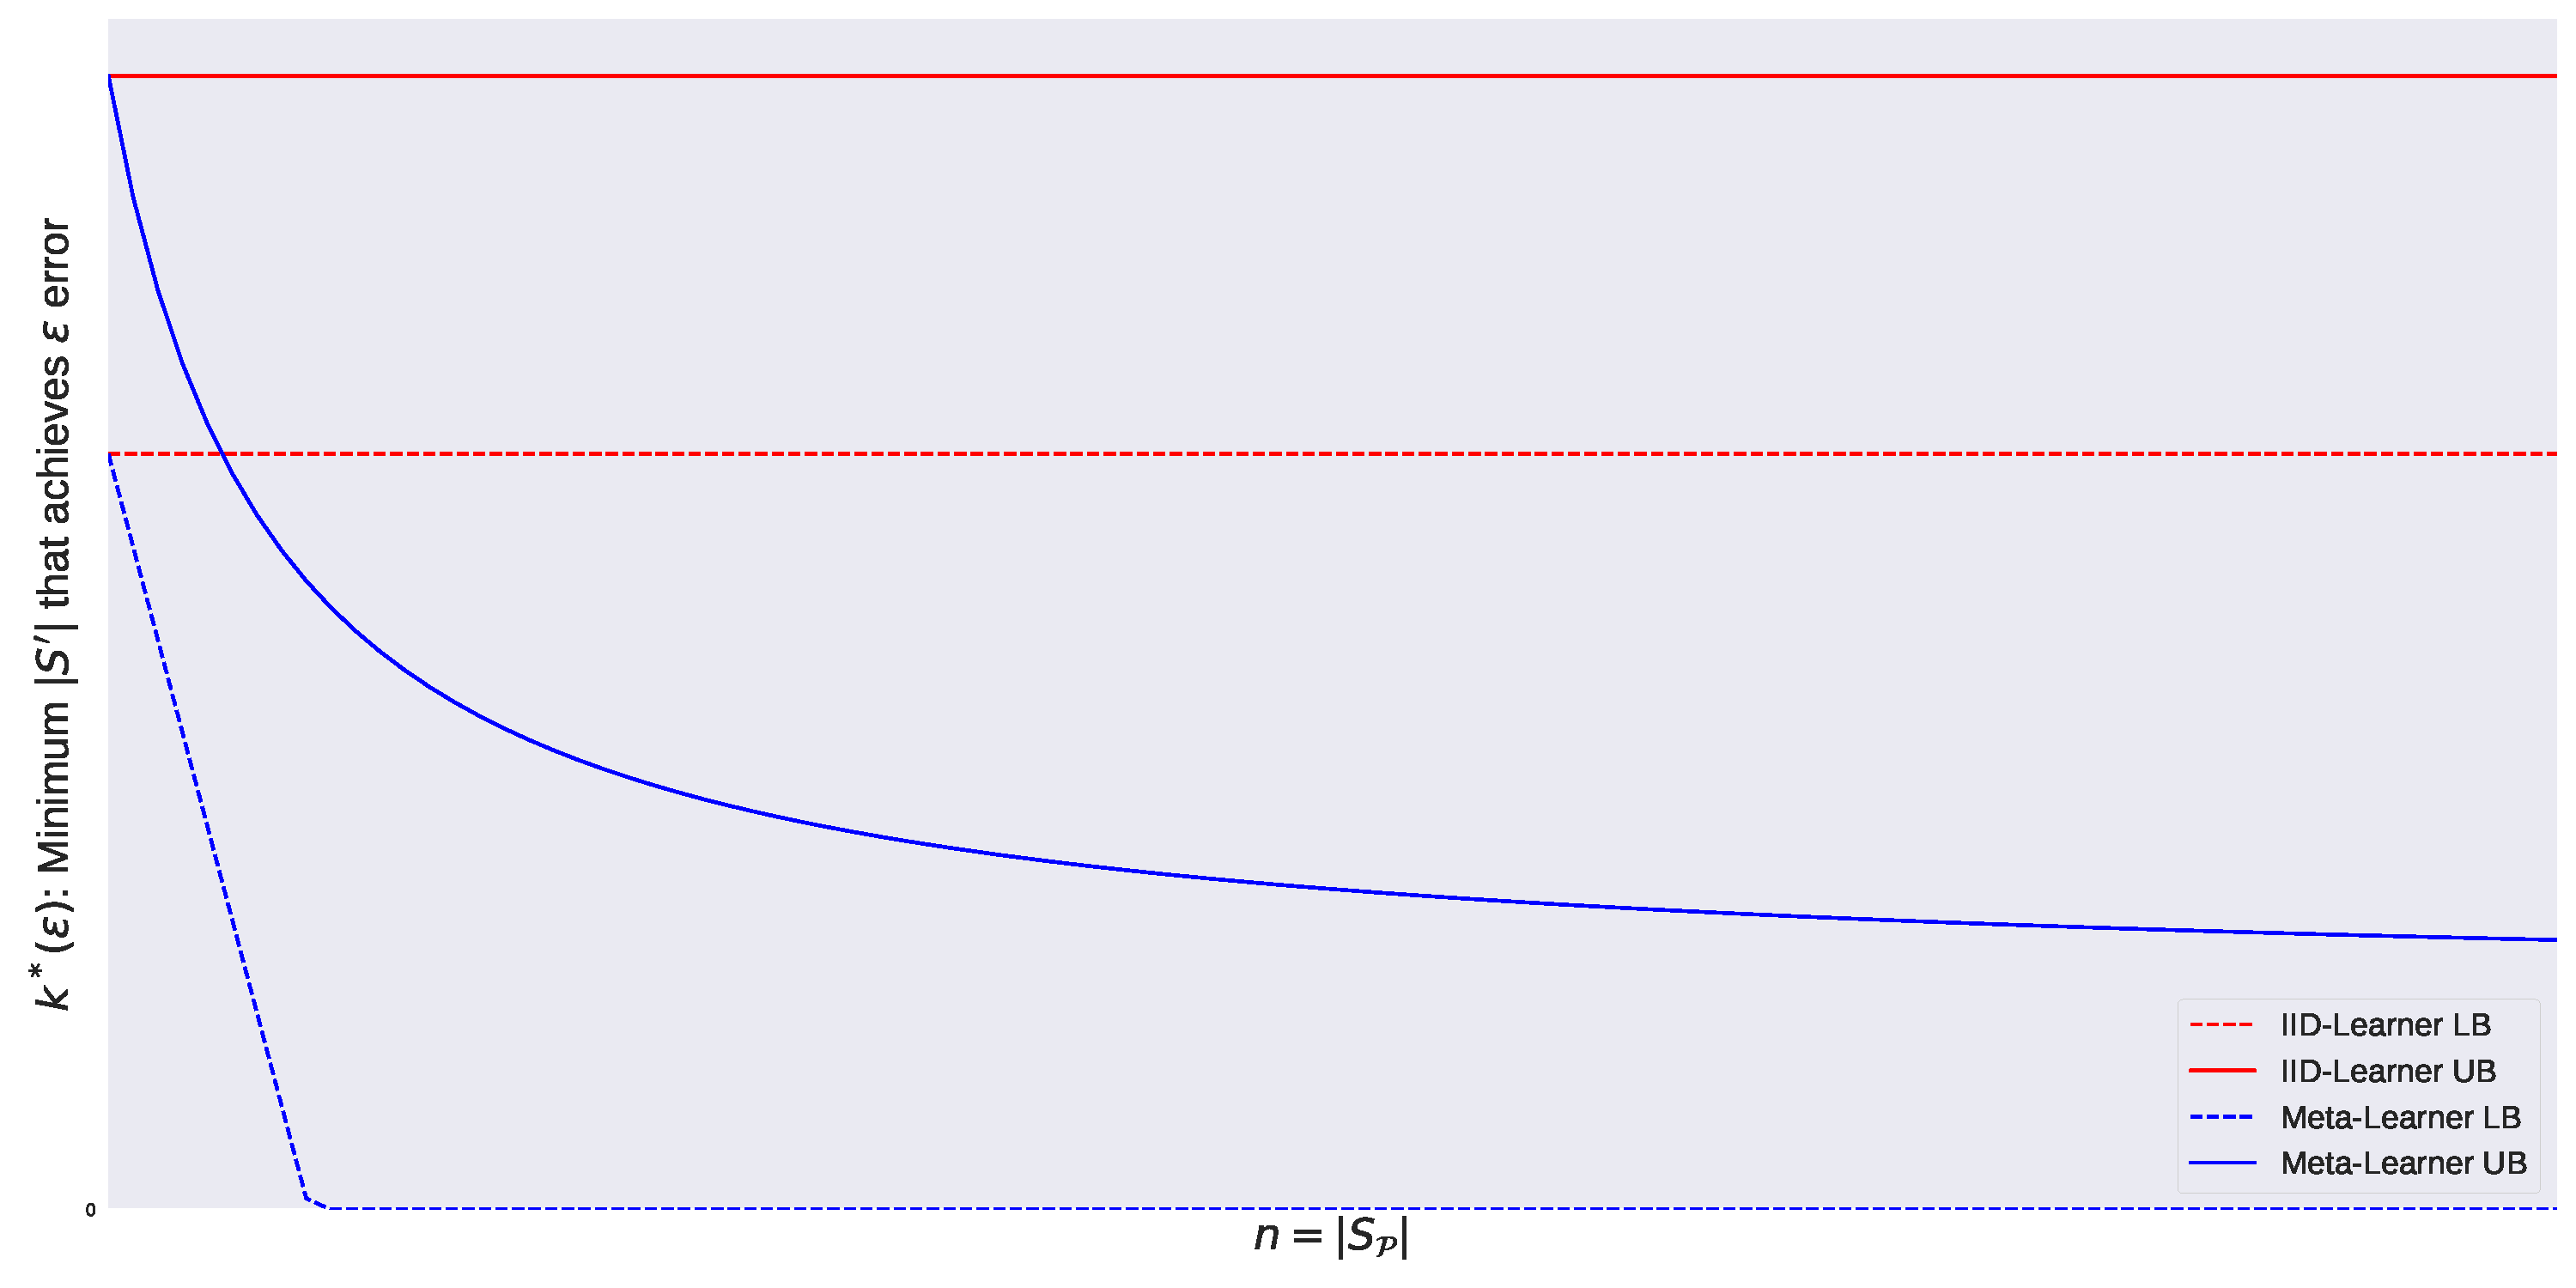
\includegraphics[width=\linewidth]{main/images/min_k_bounds_plot.pdf}\vspace{-0.5cm}
\caption{\textbf{Simulated error bounds for meta-learners} We illustrate the overall relationship between the theoretical bounds we derive in this work. On the $y$-axis, we plot the minimum number of samples needed from the novel task to achieve an $\epsilon$-error threshold. The bounds for an \iid learner that ignores the additional data, $\envS$, is shown in red while the meta-learning bounds we derive are illustrated in blue. We simulate these bounds using our derived results.
%and hand-selecting suitable constants 
Note that we chose constants to 
place the bounds for these two different learners on a similar scale, so the scale of the bounds relative to each other is uninformative.}
\label{fig:learning_bounds}
\end{figure}

\section{Summary of results}
\label{sec:summary}

\JL{Convert to bullet points in intro and remove this}

Lower bounds on the error of statistical estimation problems allow us to determine the gap between
the performance of specific learning algorithms and the theoretically best achievable error. If the
generalization upper bound and lower bound (asymptotically) match, then we know that the learning
algorithm is (asymptotically) optimal for this learning problem.

In Sections \ref{sec:minimax_setting} and \ref{sec:lbounds}, we introduce novel lower-bounds on the minimax risk of parameter estimation for a
multi-task learning problem. These lower bound characterizes the difficulty of learning in this
setting as a function of the proportion of the task-space covered by the training data, number of
training data points, and the number of data points supporting a novel task.

We then proceed in Section~\ref{sec:hierarchical_bayes} with a study of a hierarchical Bayesian model of meta linear regression. Our aims are two-fold. First, we wish to investigate the tightness of our lower bounds in this setting using an accompanying upper bound. Second, through analyzing a simple instance of the meta-learning problem we provide some intuition into the necessary conditions for successful meta-learning in general.

Figure~\ref{fig:learning_bounds} illustrates our high-level theoretical findings. We plot the minimum number of samples needed from the novel task to achieve some error threshold. The \iid-Learner does not utilize data from $\envS$ and is therefore constant. Our lower-bounds indicate that, if the training tasks sufficiently span the environment, then with enough data from these tasks the error on any novel task can be driven to zero. However, the upper bounds we derive do not have zero error asymptotically in $|\envS|$, even when the tasks may span the entire environment. We discuss this further in Section~\ref{sec:hierarchical_bayes}.

Finally, we conclude with a qualitative empirical evaluation of the meta linear regression setting. We show that this relatively simple linear setting is able to capture key features of few-shot learning and, moreover, that these features are predicted well by our theoretical analysis.
%% !TEX root = main.tex
\section{Novel task environment risk}
\label{sec:minimax_setting}
% \vspace{-0.1in}
Most existing theoretical work studying out-of-distribution generalization focuses on providing upper-bounds on generalization performance \citep{ben2010theory, pentina2014pac, amit2017meta}. We begin by instead exploring the converse: what is the best performance we can hope to achieve on any given task in the environment? After introducing notation and minimax risks, we then show how these ideas can be applied, using meta linear regression as an example.
%problem.

A full reference table for notation can be found in Appendix~\ref{app:notation} and a short summary is given here.
We consider algorithms that learn in an environment $(\spaceZ, \calP)$, with data domain $\spaceZ = \spaceX \times \spaceY$ and $\calP$ a space of distributions with support $\spaceZ$. In the typical \iid setting, the algorithm is provided training data $S \in \spaceZ^k$, consisting of $k$ \iid samples from $P \in \calP$. 

In the standard {\it multi-task} setting, we sample training data from a set of training tasks $\{P_1,\ldots,P_{M+1}\} \subset \calP$.
We extend this to a meta-learning, or {\it novel-task} setting by first drawing $\envS$: $n$ training data points from the first $M$ distributions, for a total of $nM$ samples. We call this the {\it meta-training set}. We then draw a small sample of novel data,
called a {\it support set}, $\testS \in \spaceZ^k$, from $P_{M+1}$. 
%Throughout, we use $P^k$ to denote the %product distribution, whose samples %correspond to $k$ independent samples from %$P$.

Consider a symmetric loss function $\lossfn(a,b) = \monofn(\metricfn(a, b))$ for non-decreasing $\monofn$ and arbitrary metric $\metricfn$. We seek to estimate the output of $\theta: \calP \rightarrow \Omega$, a functional that maps distributions to a metric space $\Omega$. For example, $\theta(P)$ may describe the coefficient vector of a high-dimensional hyperplane when $\calP$ is a space of linear models, and $\metricfn$ may be the Euclidean distance.

\paragraph{The \iid minimax risk} Before studying the meta-learning setting, we first begin with a definition of the \iid minimax risk that measures the worst-case error of the best possible estimator,
\begin{equation}\label{eqn:iid_risk}
    R^* = \inf_{\estimator}\sup_{P \in \calP}\iidexploss.
\end{equation}
For notational convenience, we denote the output of $\theta(P)$ by $\theta_P$. The estimator for $\theta$ is denoted, $\estimator: \spaceZ^k \rightarrow \Omega$, and maps $k$ samples from $P$ to an estimate of $\theta_P$.

\paragraph{Novel-task minimax risk} In the novel-task setting, we wish to estimate $\theta_{P_{M+1}}$, the parameters of the novel task distribution $P_{M+1}$.
We consider two-stage estimators for $\theta_{P_{M+1}}$. In the first stage, the meta-learner uses a learning algorithm $f: \envS \mapsto \bestimator_{\envS}$,  that maps the meta-training set to an estimation algorithm, $\bestimator_{\envS}:~\spaceZ^k\rightarrow~\Omega$. In the second stage, the learner computes $\bestimator_{\envS}(\testS)$, the estimate of $\theta_{P_{M+1}}$.

The novel-task minimax risk is given by, 
\begin{equation}\label{eqn:novel_risk}
    R^*_\calP(\beta) = \inf_{f} \sup_{P_1,\ldots,P_{M+1} \in \calQ^{\beta}_{\calP}} \envexploss{P_{1:M}}{P_{M+1}}{\envS}{\testS},
\end{equation}
where $\calQ^{\beta}_{\calP} = \{(P_1,\ldots,P_{M+1}) \in \calP : \KL{P_{M+1}}{P_i} \leq \beta, \textrm{ for } i=1,\ldots,M\}$. This ensures a degree of relatedness between the novel and meta-training tasks.

The estimator for $\theta_{M+1}$ now depends additionally on the $Mn$ samples in $\envS$, where only $k\ll~Mn$ samples from $P_{M+1}$ are available to the learner. Thus, $R^*_\calP$ addresses the domain shift expected at test-time in the meta-learning setting and allows the learner to use data from multiple tasks. The goal of $f$ is to learn an inductive bias from $\envS$ such that a good estimate is possible with only $k$ data points from $P_{M+1}$. In this setting, $k$ is equivalent to the number of shots in few-shot learning.

% We will begin by reviewing lower-bounds on the minimax risk for the \iid setting and then extend these results to the environment minimax risk.
%% !TEX root = main.tex
\paragraph{An example with meta-linear regression}
We present here a short summary based on meta linear regression, which we will analyze
in more detail in Section~\ref{sec:hierarchical_bayes}.

\begin{figure}
% \begin{minipage}{.5\textwidth}
%     \centering
%     % \fbox{
%     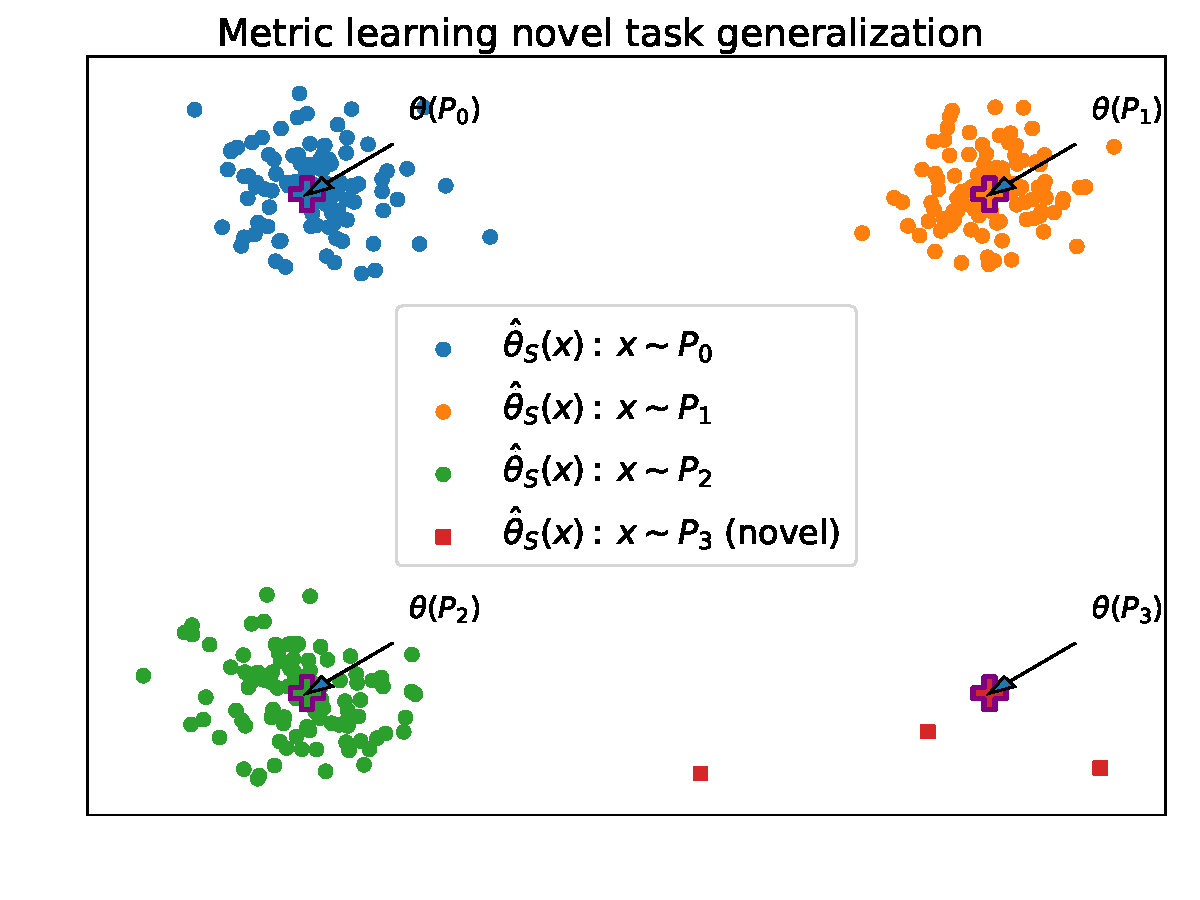
\includegraphics[width=\linewidth]{images/metric_learning_env.pdf}
%     % }
%     \caption{\textbf{Metric learning (synthetic):} An embedding function is estimated that is on-average close to a true representation of each task (`+'). The embeddings are shown compared to the target representation for each task distribution.}
%     \label{fig:metric_learning_env}
% \end{minipage}
% \begin{minipage}{\textwidth}
% \centering
% \fbox{
\iflatexml
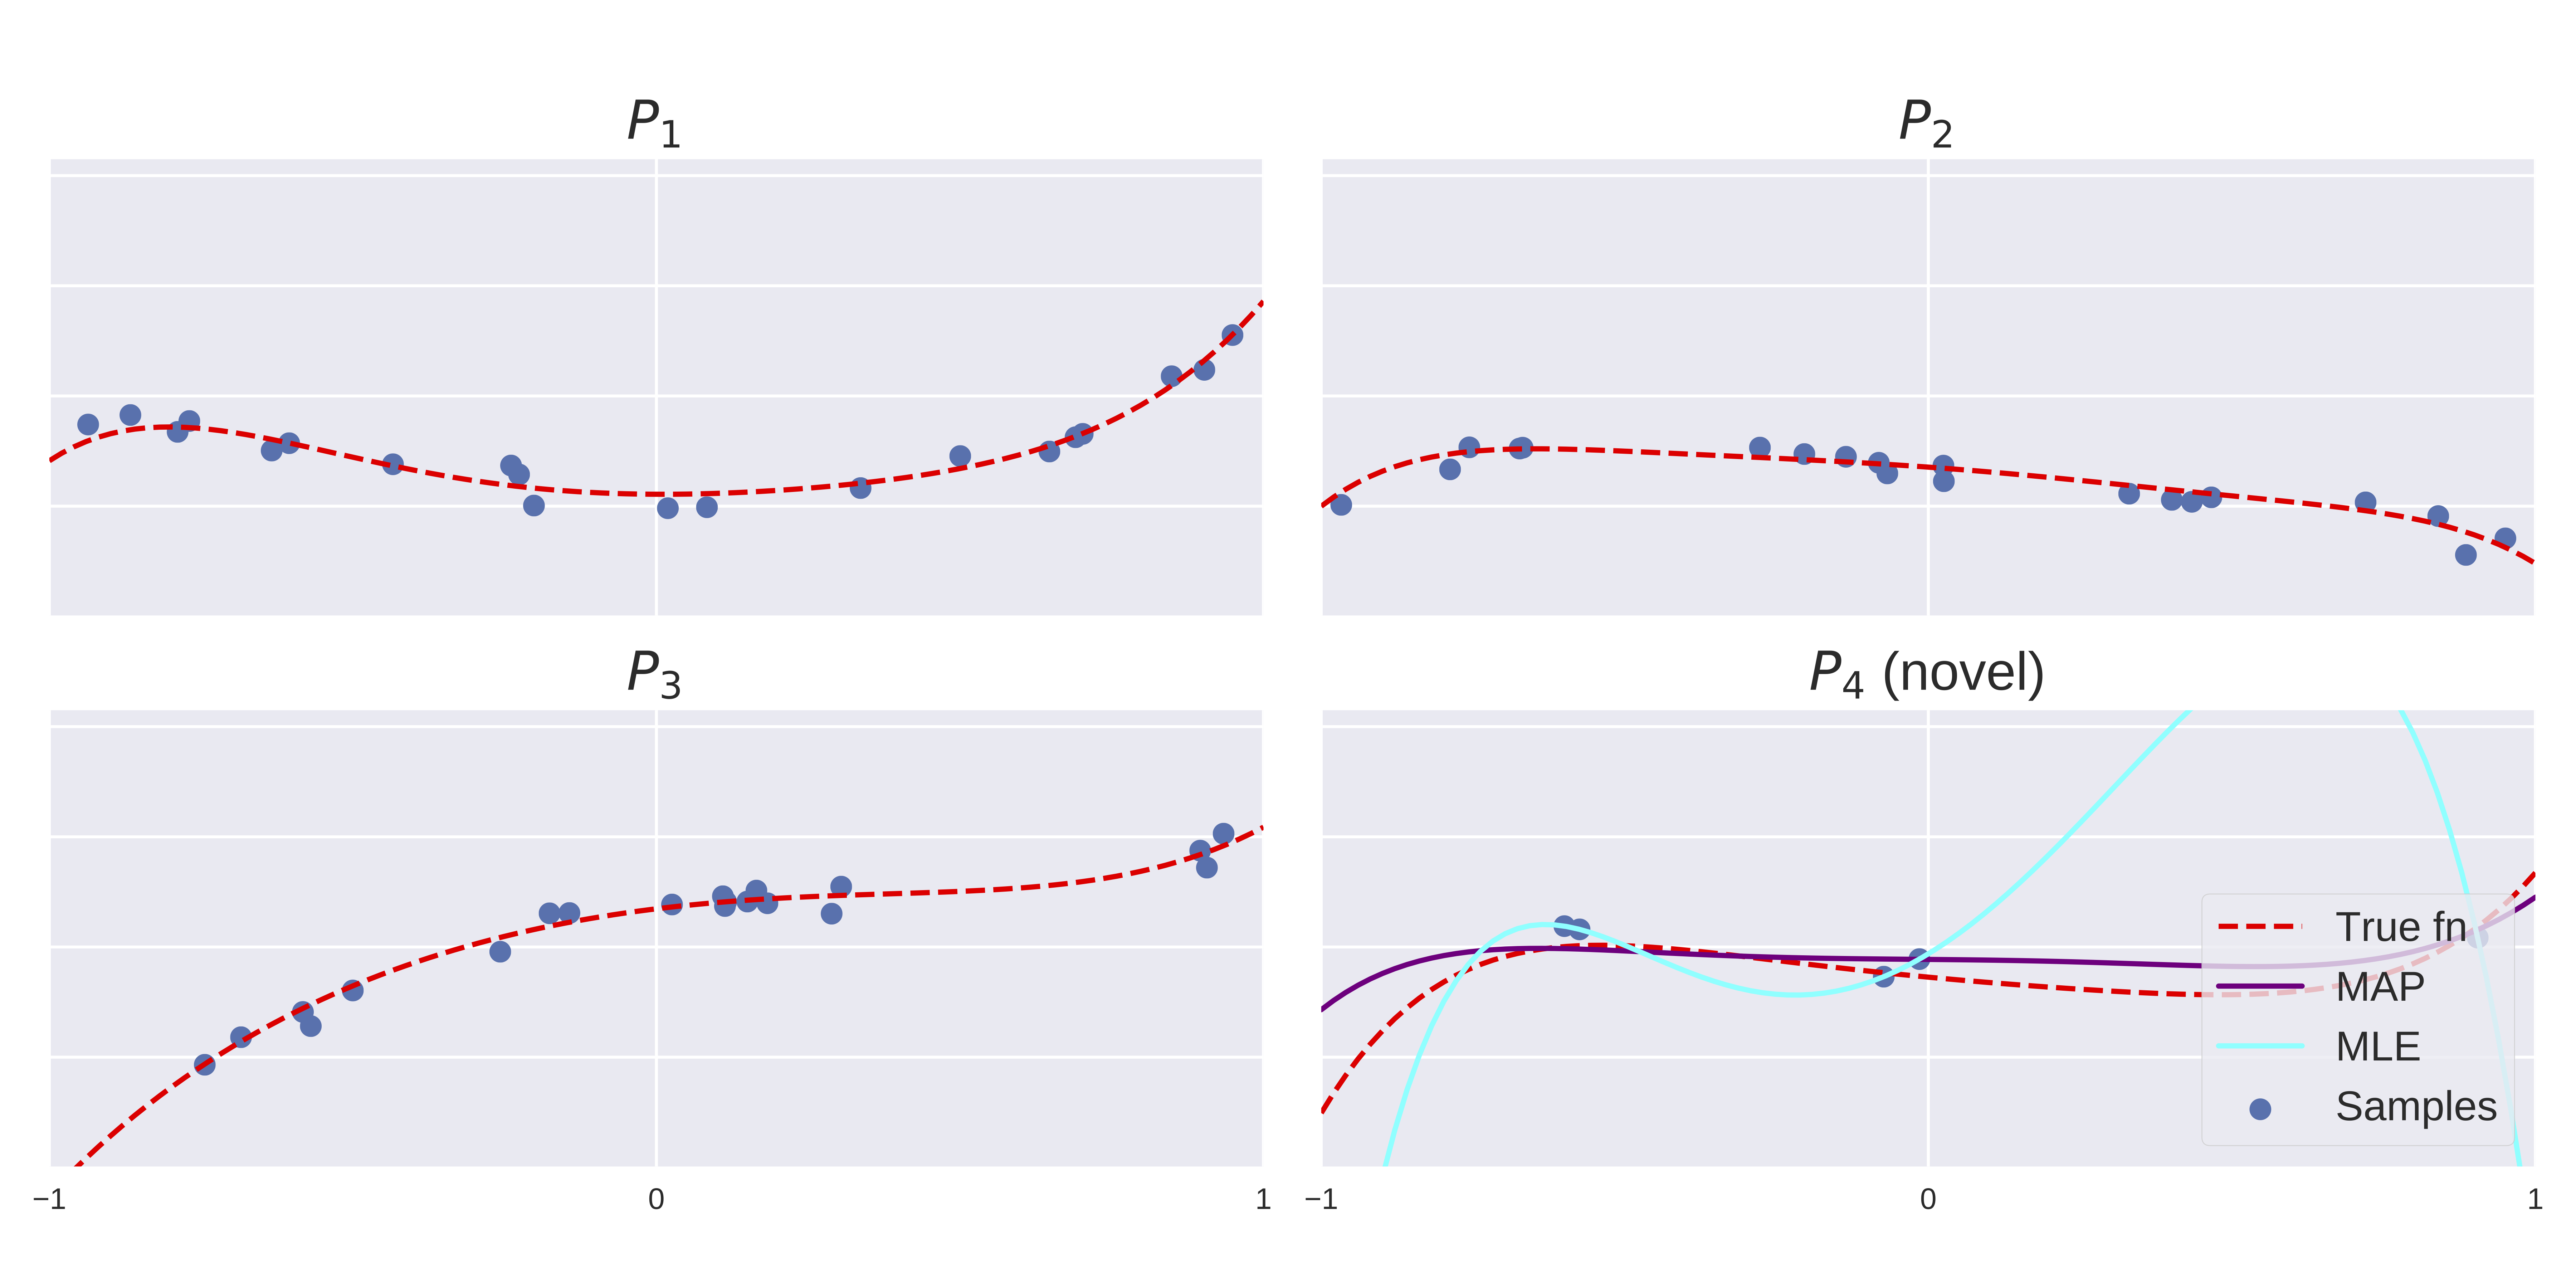
\includegraphics[width=6\linewidth]{main/images/meta_regression.png}%
\else
\centering
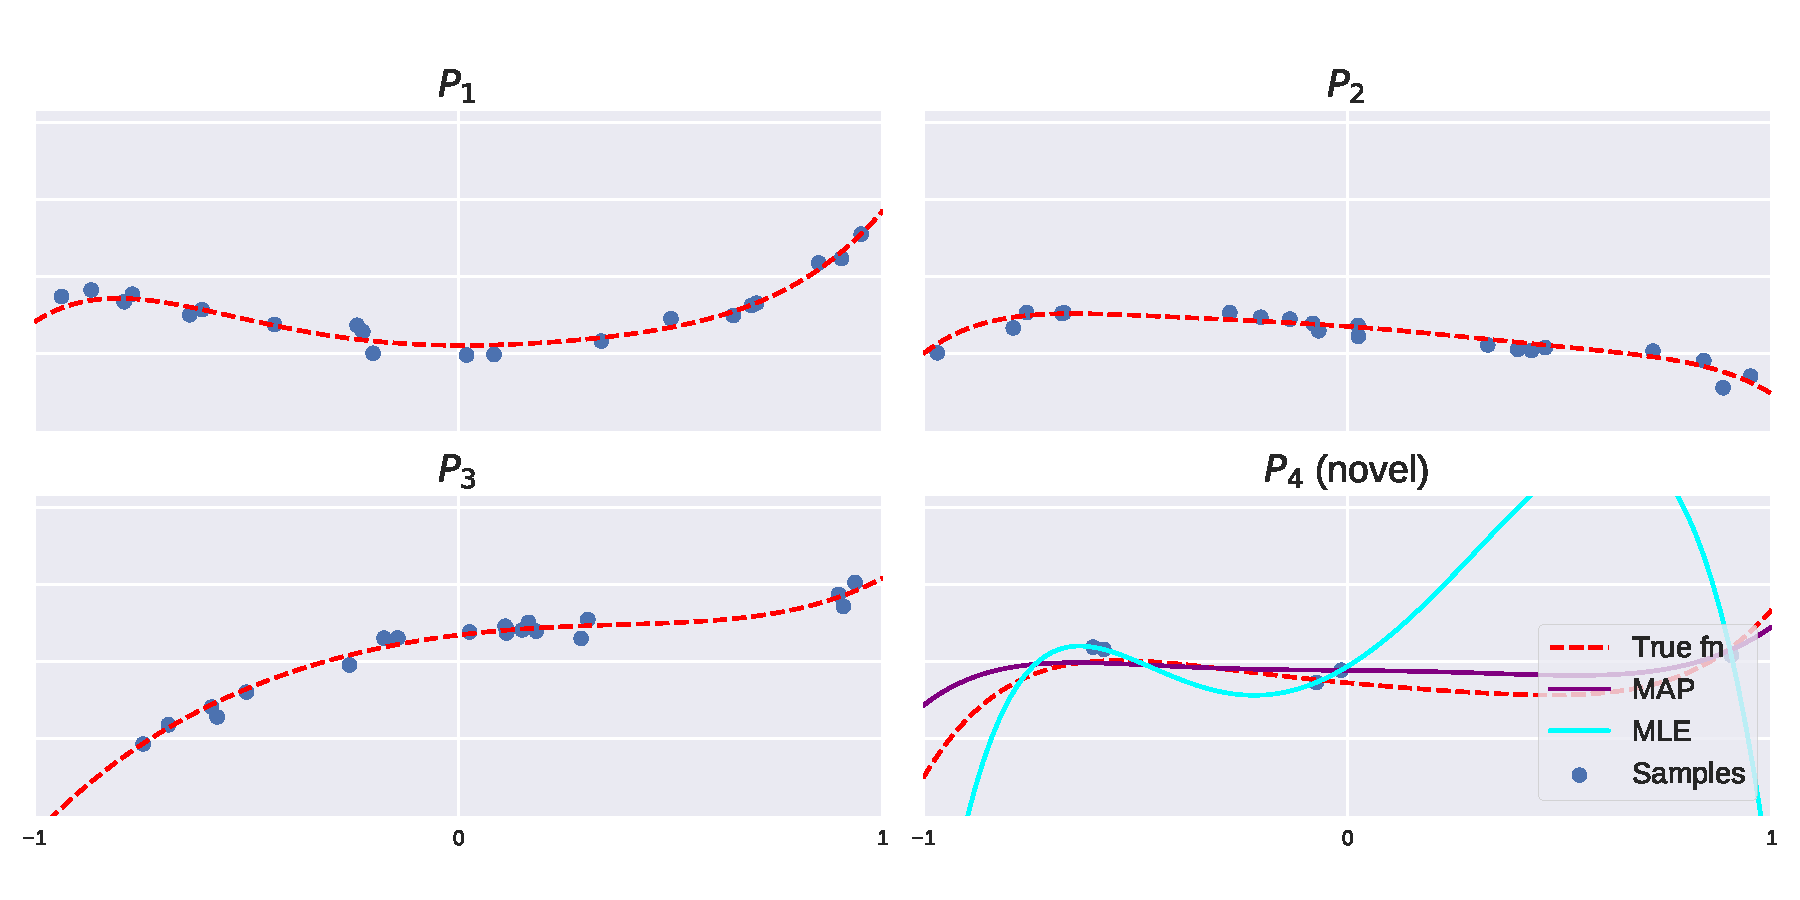
\includegraphics[width=\linewidth]{main/images/meta_regression.pdf}%
\fi
% }
\caption{\textbf{Meta-learning 1D-regression:} The parameters of a 1D regression model are fitted
from a small support set. The training distributions ($P_1,P_2,P_3$) give a useful inductive bias
for fitting $P_4$ using only 5 points. The MLE solution on the novel task for those 5 points is also
displayed.}
\label{fig:meta_lin_ref}
% \end{minipage}
\end{figure}
In Figure~\ref{fig:meta_lin_ref}, we show observed data samples from a family of polynomial
regression models. Our aim is to output an algorithm which recovers the parameters of a new polynomial function from limited observations--we choose a MAP estimator which is described fully in
Section~\ref{sec:hierarchical_bayes}. In the bottom right, we are given only 5 data points from a
novel task distribution and estimate the parameters of the model with both the MLE and MAP
estimators --- the MLE overfits the support set while the MAP estimator is close to the true function.

In terms of the terminology used above, the set,
\[\calP = \{p_{\lregparams}(y)=\calN(\bx^\top \lregparams,\sigma^2): \lregparams \in \bbR^{d}, \bx=[1,x,\ldots,x^{d-1}]\},\]
is the space of polynomial regression models, parameterized by $\lregparams$. For this problem, we take $\lossfn(\estimator, \theta) = \norm{\estimator - \theta}_2^2$. In Figure~\ref{fig:meta_lin_ref}, tasks are generated with $p(\theta) = \calN(\tau, \sigma^2_\theta)$, for unknown, sparse, $\tau \in \bbR^d$. Thus, each model is a polynomial function with few large coefficients. The algorithm $f$, first takes samples from $P_1,P_2,P_3$ and computes an estimate, $\hat{\tau}$. This estimate of $\tau$ is then used to compute $\bestimator(\testS; \hat{\tau}) = \argmax_{\lregparams_4} p(\lregparams_4|\hat{\tau}, \testS)$. Note that this approach is able to learn the correct inductive bias from the data, without requiring a carefully designed regularizer.  The lower bounds we derive in Section~4 can be applied to problems of this general type, and the upper and lower bounds in Section~5 apply specifically to meta-learning linear regression.
%
\section{Information theoretic lower bounds on novel task generalization}
\label{sec:lbounds}
\vspace{-0.1in}

In this section, we first present our most general result: Theorem~\ref{thm:env_lower_bound}. Using this, we derive Corollary~\ref{corollary:env_lbound_packing} that gives a lower bound in terms of the sample size in the training and novel tasks. Corollary~\ref{corollary:env_lbound_packing} recovers a well-known \iid lower bound (Theorem~\ref{thm:lower_bound}) when $Mn=0$, and, importantly, highlights that the novel task data is significantly more valuable than the training task data. Additionally, we provide a specialized bound that applies when the environment is partially observed --- proving that in this setting training task data is insufficient to drive the minimax risk to zero.

In Theorem~\ref{thm:env_lower_bound}, we assume that $\calP$ contains $J$ distinct $2\delta$-separated distributions but only $M+1 \leq J$ tasks are visible to the learner. Intuitively, the error rate lower-bound shrinks as the amount of information shared between the training tasks and the novel task grows.
All proofs are given in Appendix~\ref{app:proofs:lbounds}. Recall $\lossfn(a,b) = \monofn(\metricfn(a, b))$ for non-decreasing $\monofn$ and arbitrary metric $\metricfn$.

\begin{restatable}[Minimax novel task risk lower bound]{theorem}{envlbound}\label{thm:env_lower_bound}
Let $\calJ \subset \calP$ contain $J$ distinct distributions such that $\metricfn(\theta_{P}, \theta_{P'})~\geq~2\delta$ and $\KL{P}{P'} \leq \beta$ for all $P,P' \in \calJ$. 
Let $\pi$ be a random ordering of the $J$ elements, and $Z|\pi$ be a vector of $k$ \iid samples from $P_{\pi_{M+1}}$.
Further, define $W|\pi$ to be an $n \times M$ matrix whose $j^{th}$ column consist of $n$ \iid samples from $P_{\pi_j}$. Then,
\begin{align*}
R^*_\calP(\beta) \geq
\monofn(\delta)\left(1 - \dfrac{I(\pi_{M+1}; W) + I(\pi_{M+1};Z) + 1}{\log_2 J}\right).
\end{align*}
\end{restatable}
Note that $\delta$ is a property of the so-called packing set, $\calJ$, and may depend on the sample size, $\beta$, and other properties of $\calP$. For example, practical instances of this bound typically require $\monofn(\delta) = O(1/k)$ or similar, as in Theorem~\ref{thm:mlreg_lower_bound} below.
To derive this result, we bound the statistical estimation error by the error on a corresponding decoding problem where we must predict the novel task index, given the meta-training set $\envS$ and $\testS$. Fano's inequality provides best-case error rates for this problem.

% % !TEX root = main.tex

\paragraph{Lower bounding with local packing} The lower bound of Theorem~\ref{thm:env_lower_bound} requires a difficult computation of the information shared between the samples and the identity of the novel task distribution. To alleviate this difficulty, we introduce a local packing bound on the information.

\begin{restatable}[Meta-learning local packing]{lemma}{looproductpacking}\label{lemma:env_local_product_packing}
Consider the same setting as in Theorem~\ref{thm:env_lower_bound}, then
\[I(\pi_{M+1}; W) \leq \frac{Mn}{J^2(J-1)} \sum_{1 \leq i,j \leq J} \KL{P_{i}}{P_{j}}\]
\end{restatable}



% Combining Theorem~\ref{thm:env_lower_bound}, Lemma~\ref{lemma:env_local_product_packing}, and a standard \iid local packing bound on $I(\pi_{M+1}; Z)$ (Lemma~\ref{lemma:local_packing}, Appendix~\ref{app:proofs}) we recover a bound on the novel-task minimax risk that depends on the number of tasks and datapoints per task.
Using Theorem~\ref{thm:env_lower_bound}, we derive our first bound on the novel-task minimax risk that depends on the number of meta-training tasks ($M$) and datapoints per training task ($n$, $k$), via a local-packing argument. The following corollary implies that if we have $J$ meta-training tasks in our $2\delta$-packing that are close
(in terms of their pairwise KL distance), then learning a novel task from training samples drawn
from the meta-training tasks requires significantly more examples; in particular, learning the novel task from samples drawn from the
meta training set requires  $\Omega(J)$ times the sample complexity of the novel task. This matches our intuition that learning the novel task implies the ability to distinguish it from all $J$ well-separated meta-training tasks.
\begin{restatable}[]{corollary}{envlboundpacking}\label{corollary:env_lbound_packing}
Assume the same setting as in Theorem~\ref{thm:env_lower_bound}. Then,
\begin{align*}
R^*_\calP(\beta) \geq \monofn(\delta) \left(1 - \dfrac{1 + \left(\frac{Mn}{(J-1)} + k\right)\frac{1}{J^2}\sum_{1 \leq i,j \leq J}\KL{P_i}{P_j}}{\log_2 J}\right).
\end{align*}
\end{restatable}

\paragraph{A tighter bound on partially observed environments} We now consider the special case of Theorem~\ref{thm:env_lower_bound} when $M < J-1$, meaning that the meta-training tasks cannot cover the full packing set. In this setting, we prove that no algorithm can generalize perfectly to tasks in unseen regions of the space with small $k$, regardless of the number of data points $n$ observed in each meta-training task.

\begin{restatable}[]{corollary}{envlboundasymp}\label{thm:env_lower_bound_asymp}
Assume the same setting as in Theorem 1, with $M+1 < J$. Then,
\begin{align*}
R^*_\calP \geq \monofn(\delta)\left(\dfrac{\log_2 (J - M) - \frac{k}{J^2}\sum_{1 \leq i,j \leq J}\KL{P_i}{P_j} - 1}{\log_2 J}\right).
\end{align*}
\end{restatable}

In this work, we have focused on the setting where $W$ contains an equal number of samples from each of the meta-training tasks --- this is the sampling scheme shown in Figure~2. However, it is possible to extend these results to different sampling schemes for $W$. For example, in the appendix we derive bounds with $W|\pi$ as a mixture distribution. Surprisingly, despite task identity being hidden from the learner, the asymptotic rate for these two sampling schemes match.

\subsection{Measuring Task-Relatedness}

The use of local packing requires the design of an appropriate set of distributions whose corresponding parameters are $2\delta$-separated but maintain small KL divergences. In the multi-task setting such an assumption is intuitively reasonable: challenging tasks should require separated parameters for ideal explanations ($2\delta$-separated) but should satisfy some relatedness measure (small KL). Importantly, these parameters can depend on sample size and other problem-specific variables. As we will see shortly, lower bounds on minimax risk in the \iid setting may also assume the same notion of relatedness for the local-packing in $\calP$.

Task relatedness is a necessary feature for upper-bounds on novel task generalization, but are typically difficult to define (see e.g. \citet{ben2008notion}). Our lower bounds utilize a relatively weak notion of task-relatedness, and thus may be overly pessimistic compared to the upper bounds computed in existing work. However, task relatedness of this form can be formulated in a representation space shared across tasks and thus can be applied in settings like those explored by e.g. \citet{du2020few}. Deriving lower bounds under the different task relatedness assumptions present in the literature would make for exciting future work.

\subsection{Comparison to risk of \iid learners}

From the statement of Theorem~\ref{thm:env_lower_bound} it is not clear how this lower-bound compares to that of the \iid learner which has access only to the $k$ samples from $\testS$.
To investigate the benefit of additional meta-training tasks, we compare our derived minimax risk lower bounds to those achieved by \iid learners. To do so, we revisit standard minimax lower bounds that can be found in e.g. \citet{loh2017lower}. 

\begin{restatable}[IID minimax lower-bound]{theorem}{iidlbound}\label{thm:lower_bound}
Suppose $\{P_1,\dots,P_J\} \subseteq \calP$ satisfy $\metricfn(\theta_{P_i}, \theta_{P_j}) \geq 2\delta$ for all $i\neq j$. Then,
\begin{align*}
R^* \geq \monofn(\delta)\left(1 - \dfrac{\frac{k}{J^2}\sum_{1 \leq i,j \leq J}\KL{P_i}{P_j} + 1}{\log_2 J}\right).
\end{align*}
\end{restatable}

We include a proof of this result in Appendix~\ref{app:proofs:lbounds}, using local-packing as in our meta-learning bounds. As hoped, Corollary~\ref{corollary:env_lbound_packing} recovers Theorem~\ref{thm:lower_bound} when there are no training tasks available. Moreover, this \iid bound is strictly larger than the one computed in Corollary~\ref{corollary:env_lbound_packing} in general. Note that while this \iid minimax risk is asymptotically tight for several learning problems \citep{loh2017lower, raskutti2011minimax}, there is no immediate guarantee that the same is true for our meta-learning minimax bounds. We investigate the quality of these bounds by providing comparable upper bounds in the next section.
%% !TEX root = main.tex

\section{Analysis of a hierarchical Bayesian model of meta-learning}
\label{sec:hierarchical_bayes}

Our goal is to analyze the sample complexity of meta-learning for linear regression, where samples are drawn from multiple meta-training tasks and we want to generalize to a new task with only a few data points. After introducing the setting, we will compute lower-bounds on the minimax risk using our results from Section~\ref{sec:lbounds}, revealing a $2^{d}$ scaling on the meta-training sample complexity. Following the lower bound, we derive an accompanying upper-bound on the risk of a MAP estimator, derived from an empirical Bayes estimate over a hierarchical Bayesian model. Asymptotic analysis of this bound reveals that if the observed samples from the novel task vary considerably more than the task parameters, then observing more meta-training samples may significantly improve convergence in the small $k$ regime. This is validated empirically in Section~\ref{sec:empirical}.

% \begin{minipage}[t]{0.48\linewidth}
For $i = 1...M+1$, where $M+1$ is the total number of tasks, we define,
\begin{align*}
\by_i      &= X_i\lregparams_i + \beps_i, &&  X_i \in \bbR^{n_i \times d}, \by_i \in \bbR^{n_i}, \beps_i \in \bbR^{n_i} \\
\beps_i &\sim \mathcal{N}(0, \sigma^2_i I), && \sigma^2_i \in \bbR^{+}
\end{align*}
Each task has some design matrix $X_i$ and unknown parameters $\lregparams_i$. For simplicity, we assume known isotropic noise models and that $n_i = \nX$ for all $i\leq M$, with $n_{M+1}=\nY$.

Our meta learner will fit the data using an empirical Bayes estimate in a hierarchical Bayesian model:
\begin{align*}
\lregparams_i = \btau + \bxi, \:\:\:\: \btau \in \bbR^{d},\:\:\:\: \bxi \in \bbR^{d},
\:\:\:\: \bxi \sim \mathcal{N}(0, \sigma^2_\theta I),\:\:\:\: \sigma^2_\theta \in \bbR^{+}
\end{align*}

% \end{minipage}\hfill%
% \begin{minipage}[t]{0.48\linewidth}
% \centering
%     \strut\vspace*{-\baselineskip}\newline
%     \begin{tikzpicture}[
%     roundnode/.style={circle, draw=gray, very thick, minimum size=8mm},
%     observednode/.style={circle, draw=gray, fill=gray!25, very thick, inner sep=2pt},
%     ]
%     %Nodes
%     \node[roundnode]        (tau)                              {$\tau$};
%     \node[roundnode]        (thetax)       [below left=0.8cm and 1.2cm of tau] {$\btheta_1$};
%     \node[roundnode]        (thetay)       [below right=0.8cm and 1.2cm of tau] {$\btheta_2$};
%     \node[observednode]     (x1)       [below left=0.8cm and 0.5cm of thetax] {$\by^{(1)}_1$};
%     \node[observednode]     (xn)       [below right=0.8cm and 0.5cm of thetax] {$\by^{(n)}_1$};
%     \node[observednode]     (y1)       [below left=0.8cm and 0.5cm of thetay] {$\by^{(1)}_2$};
%     \node[observednode]     (yk)       [below right=0.8cm and 0.5cm of thetay] {$\by^{(k)}_2$};
     
%     %Lines
%     \draw[->] (tau) -- (thetax);
%     \draw[->] (tau) -- (thetay);
%     \draw[->] (thetax) -- (x1.north);
%     \path (x1) -- node[auto=false]{\ldots} (xn);
%     \draw[->] (thetax) -- (xn.north);
%     \draw[->] (thetay) -- (y1.north);
%     \path (y1) -- node[auto=false]{\ldots} (yk);
%     \draw[->] (thetay) -- (yk.north);
    
%     \end{tikzpicture}
%     \captionof{figure}{A simple two-task hierarchical model.}
%     \label{fig:hierachical_gaussian_model}
% \end{minipage}



We will consider the Maximum a Posterior estimator,
\[\bestimatorNovel = \argmax_{\thetaY}p(\thetaY|\by_1,\ldots,\by_{M+1}),\]
and will characterize its risk, $\bbE[\norm{\bestimatorNovel~-~\thetaY}_2^2]$, where the expectation is with respect to sampled data only. The posterior distribution under the Empirical Bayes estimate for $\btau$ is given in Appendix~\ref{app:proofs:ubounds}. The derivation is standard but dense and we recommend dedicated readers to consult \citet{gelman2013bayesian}, or an equivalent text, for more details.

\subsection{Minimax lower bounds}

We now compute lower bounds for parameter estimation with meta-learning over multiple linear regression tasks.
% To do so, we first formalize this setting using the terminology and notation of prior sections.
Beginning with a definition of the space of data generating distributions,
\[\calP_{LR} = \{ p_{\lregparams}(\by) = \calN(X\lregparams, \sigma^2 I): \lregparams \in \bball_2(1), X \in \bbR^{n \times d}. \} \]

where $\lregparams$ are the parameters to be learned, and $X$ is the design matrix of each linear regression task in the environment.
% We say this in the section above
%For simplicity, we assume here that all distributions share the same, known, isotropic noise model, $\sigma I$ and that the number of data points per task is equal, $n_i = n$ for all $i < M+1$.
We write $\gamma = \max_{i} \sigma_{\max}(X_i/\sqrt{n})$, which we assume is bounded for all $X$ and $n$ (an assumption that is validated for random Gaussian matrices by \citet{raskutti2011minimax}).

\begin{restatable}[Meta linear regression lower bound]{theorem}{mlreglbound}\label{thm:mlreg_lower_bound}
Consider $\calP_{LR}$ defined as above and let $\lossfn(a,b) = (\norm{a-b}_2)^2$. If $d \geq 2$ and $2^{-d}M + kn^{-1} \geq \max\{\frac{d}{4\beta}, d\sigma^2/(256\gamma^2 n)$, then,
\[R^*_{\calP_{LR}}(\beta) \geq O\left(\frac{d\sigma^2}{\gamma^2 (2^{-d}\nX M + \nY)}\right) \]
\end{restatable}

The proof is given in Appendix~\ref{app:proofs:linear_lower}. We see that the size of the meta-training set has an inverse exponential scaling in the dimension, $d$. This reflects the complexity of the space growing exponentially in dimensions and the need for a matching growth in data size to cover the environment sufficiently.

\subsection{Minimax upper bounds}

To compute upper bounds on the estimation error, we require an additional assumption. Namely, we will assume that the design matrices also have bounded minimum singular values, $0 < s \leq \sigma_{\min}(X/\sqrt{n})$ (see \citet{raskutti2011minimax} for some justification). For the upper-bounds, we allow the bounds on the singular values of the design matrices and the observation noise in the novel task to be different than those in the meta-training tasks. We note that we can still recover the setting assumed in the lower bounds, where all tasks match on these parameters, as a special case.

The learner observes $\nX$ data points from each linear regression model in $\{ P_{\lregparams_1}, \ldots, P_{\lregparams_M} \} \subset \calP$. We then bound the error of estimating $\lregparams_{M+1}$, for which $\nY$ samples are available.

The expected error rate of the MAP estimator can be decomposed as the posterior variance and bias squared. In the appendix we provide a detailed derivation of these results. The bound depends on dimensionality $d$, the observation noise in each task $\sigma^2_i$, the number of tasks $M$, the number of data points in each meta-training task $n$, and the number of data points in the novel task $k$.

\begin{restatable}[Meta Linear Regression Upper Bound]{theorem}{mlrbv}\label{thm:lregression_bias_variance}
Let $\thetaEst$ be the maximum-a-posteriori estimator, $\muPosTheta$. Then,
\[ R^*_{\calP_{LR}} \leq \sup_{\btheta_1,\ldots,\thetaY \in \bball_2(1)}\bbE[\Vert\thetaEst - \thetaY\Vert^2] \leq O\Bigl(\dim \sigma^2_{M+1} C(M, \nX, \nY)^{-2} D(M, \nX, \nY)\Bigr) \]
where,
\[C(M, \nX, \nY) = \left[ \nY + 
\frac{M\nX}{\frac{\nX (M +\condX^2)\sminY^2}{\alphaY} + A} \right], \textrm{ and,  }D(M, \nX, \nY) = \left[ \nY + \frac{M\nX}{ 
(\frac{\nX}{\LLConst} + \MMConst ) 
(\frac{M\nX}{\LLLConst} + \MMMConst)}\right].\]
Expectations are taken over the data conditioned on $\lregparams_1,\ldots,\lregparams_{M+1}$. Additional terms not depending on $d,\:M,\:\nX,\:\nY$ are defined in Appendix~\ref{app:proofs:ubounds}.
\end{restatable}

While the bounds presented in Theorem~\ref{thm:lregression_bias_variance} are relatively complicated, we can probe the asymptotic convergence of the MAP estimator to the true task parameters, $\thetaY$. In the following section, we will discuss some of the consequences of this result and its implications for our lower bounds.

\subsection{Asymptotic behavior of the MAP estimator} 

We first notice that when $k$ is small, the risk cannot be reduced to zero by adding more meta-training data. Recent work has suggested such a relationship may be inevitable \citep{hanneke2020no}. Our lower bound presented in Corollary~\ref{thm:env_lower_bound_asymp} agrees that more samples from a small number of meta-training tasks will not reduce the error to zero. However, 
unlike our lower bounds
based on local packing, the lower bounds presented in this section predict that if the meta-training tasks cover the space sufficiently then an optimal algorithm might hope to reduce the error entirely with enough samples. We hypothesize that this gap is due to limitations in the standard proof techniques we utilize for the lower-bounds when the number of tasks grows, and expect a sharper bound may be possible.

To emulate the few-shot learning setting where $k$ is relatively small, we consider $n \rightarrow \infty$, with $k$ and $M$ fixed. In this case, the risk is bounded as,
\[\sup_{\btheta_1,\ldots,\thetaY \in \bball_2(1)}\bbE[\Vert\thetaEst - \thetaY\Vert^2] \leq O\left(\dim \sigma^2_{M+1}\left[k + \frac{2\alpha_2 M}{M + \condX^2} \right]^{-1}\right),\]
where $\alpha_2 = \smaxCY / \smaxP$, is the ratio of the observation noise to the variance in sampling $\btheta$, and $\condX$ is the condition number of the design matrices. This leads to a key takeaway: if the observed samples from $P_{M+1}$ vary considerably more than the parameters $\btheta$, then observing more samples in $\envS$ will significantly improve convergence towards the true parameters in the small $k$ regime. Further, adding more tasks (increasing $M$) also improves these constant factors by removing the dependence on the condition number, $\kappa$.




%% !TEX root = ../main.tex
\section{Experiments}
\vspace{-0.1in}
In this section, we show experimental results for our online contextualized few-shot learning
paradigm, using \ourchar{} and \ourroom{} (see Sec.~\ref{sec:benchmark}) to evaluate our model, CPM,
and other state-of-the-art methods. For Omniglot, we apply an 8$\times$8 CutOut~\citep{cutout} to
each image to make the task more challenging. 
% Details about the split information can be found in
% Appendix~\ref{app:data}.

\vspace{-0.1in} \paragraph{Implementation details:} For \ourchar{}, we use the common
4-layer CNN for few-shot learning with 64 channels in each layer. For \ourimg{}, we also use ResNet-12 
with input resolution 84$\times$84~\citep{tadam}. For the \ourroom{}, we resize the input to 
120$\times$160 and use ResNet-12. To represent
the feature of the input image with an attention mask, we concatenate the global average pooled
feature with the attention ROI feature, resulting in a 512d feature vector. For the contextual RNN,
in both experiments we used an LSTM~\citep{lstm} with a 256d hidden state. The best CPM model is
equipped using GAU and cosine similarity for querying prototypes. Logits based on cosine similarity
are multiplied with a learned scalar initialized at 10.0~\citep{tadam}. We include additional
training details in Appendix~\ref{app:exp}.

\vspace{-0.1in}
\paragraph{Evaluation metrics:}
In order to compute a single number that characterizes the learning ability over sequences, we
propose to use \textit{average precision} (AP) to evaluate
both with respect to old versus new and the
specific class predictions.
Concretely, all predictions are sorted by their old vs. new scores, and we compute AP using the area
under the precision-recall curve. A true positive is defined as the correct prediction of a
multi-class classification among known classes. We also compute the ``$N$-shot'' accuracy; i.e., the
average accuracy after seeing the label $N$ times in the sequence. Note that these accuracy scores
only reflect the performance on {\it known} class predictions. All numbers are reported with an
average over 2,000 sequences and for $N$-shot accuracy standard error is also included.
Further explanation of these metrics is in Appendix~\ref{sec:metrics}. 

\vspace{-0.1in}
\paragraph{Comparisons:}
To evaluate the merits of our proposed model, we implement classic few-shot learning and online
meta-learning methods. More implementation and training details of these baseline methods can be
found in Appendix~\ref{app:exp}.
% !TEX root = ../main.tex
\begin{figure}[t]
\vspace{-0.5in}
\centering
\iflatexml
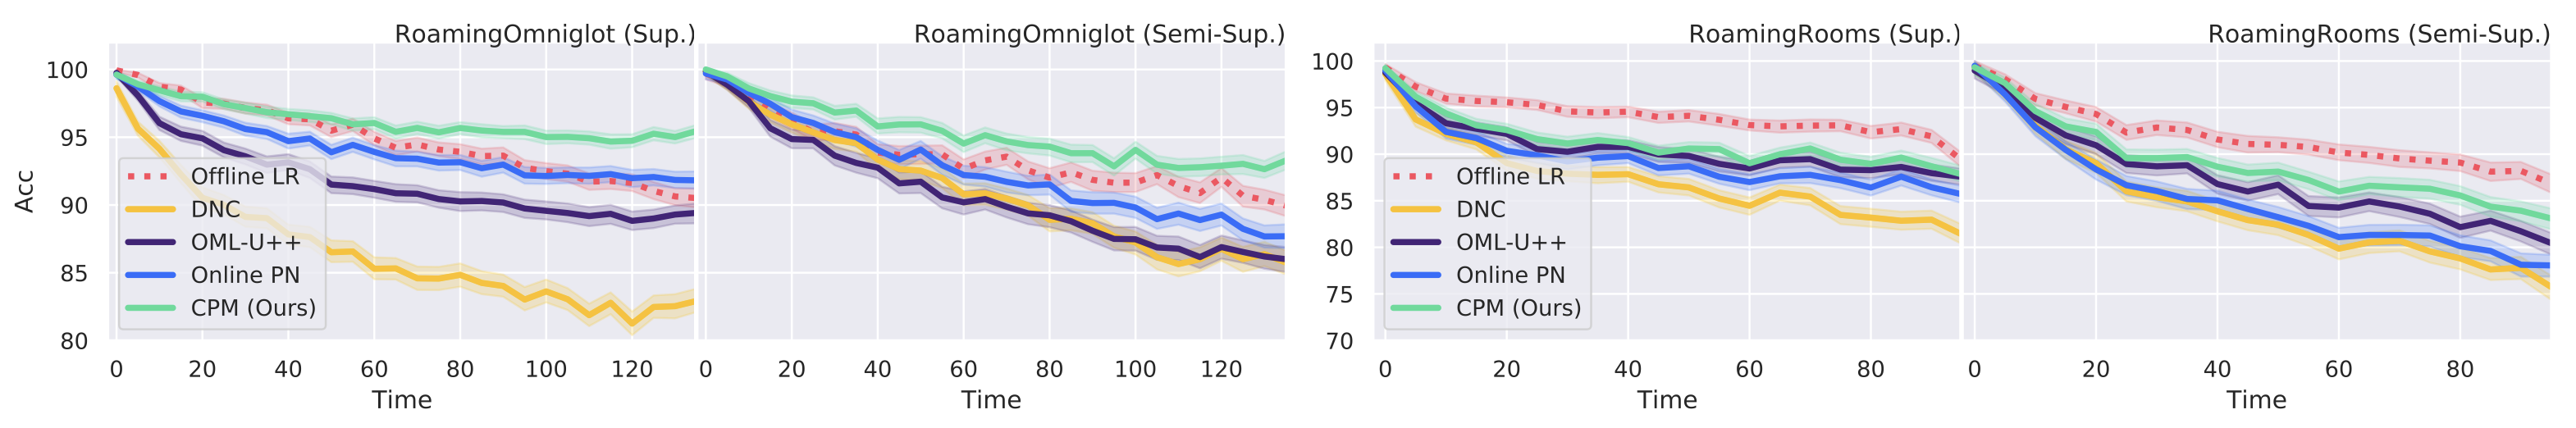
\includegraphics[width=6\linewidth]{figures/acctime_full.png}
\else
\setlength{\tabcolsep}{0pt}
\begin{tabular}{cccc}
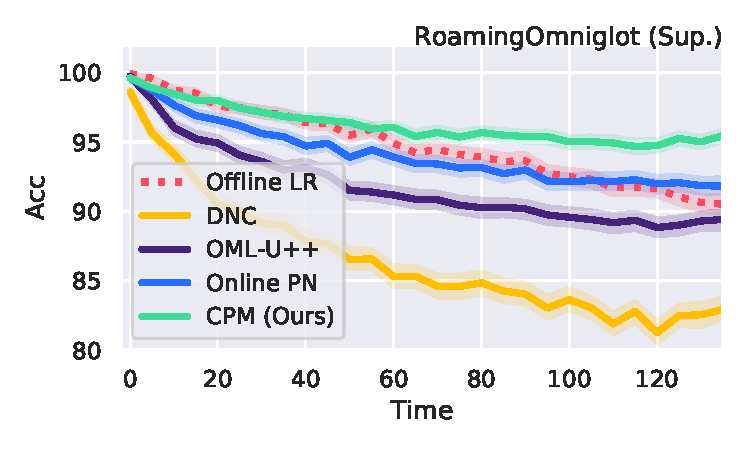
\includegraphics[height=2.4cm,trim={0.3cm 0cm 0.5cm 0},clip]{figures/omniglot-nossl-time.pdf}
&
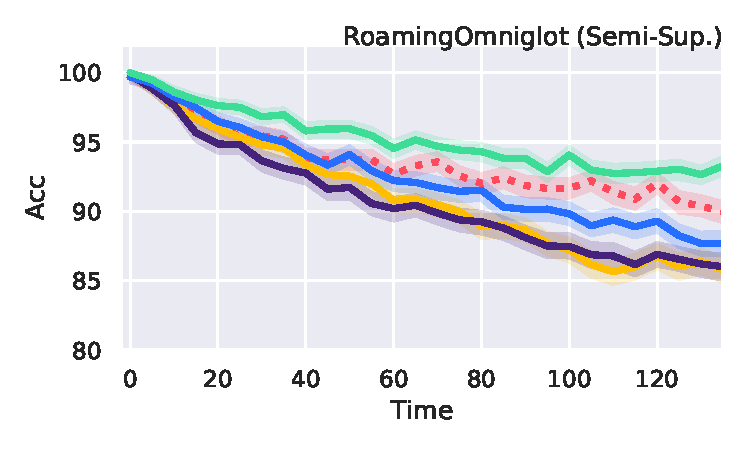
\includegraphics[height=2.4cm,trim={2cm 0cm 0cm 0},clip]{figures/omniglot-ssl-time.pdf}
&
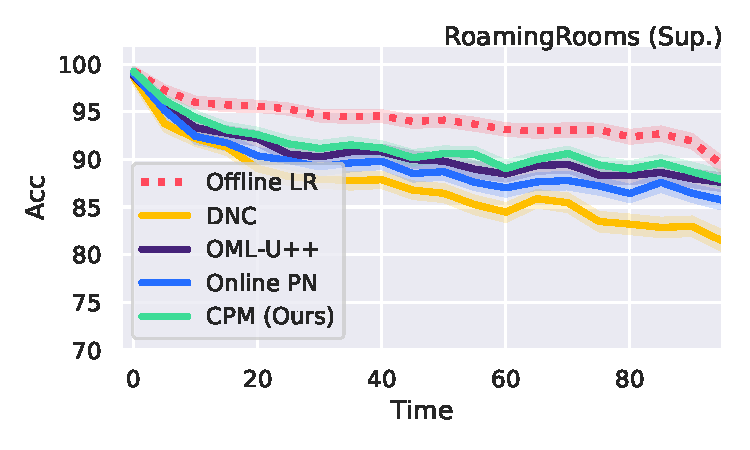
\includegraphics[height=2.4cm,trim={1cm 0cm 0.5cm 0},clip]{figures/matterport-nossl-time.pdf}
&
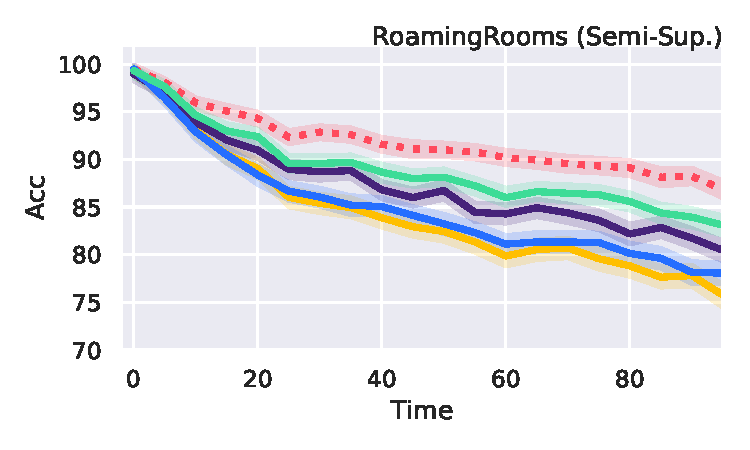
\includegraphics[height=2.4cm,trim={2cm 0cm 0cm 0},clip]{figures/matterport-ssl-time.pdf}
\\
\end{tabular}
\vspace{-0.25in}
\fi
\caption{\textbf{Few-shot classification accuracy over time.} \textbf{Left:} \ourchar{}.
\textbf{Right:} \ourroom{}. \textbf{Top:} Supervised. \textbf{Bottom:} Semi-supervised. An offline
logistic regression (Offline LR) baseline is also included, using pretrained ProtoNet features. It
is trained on all labeled examples except for the one at the current time step.}
\label{fig:acctimefull}
% \vspace{-0.25in}
\end{figure}

% !TEX root = ../main.tex
\begin{figure}[t]
\vspace{-0.1in}
\centering
\iflatexml
    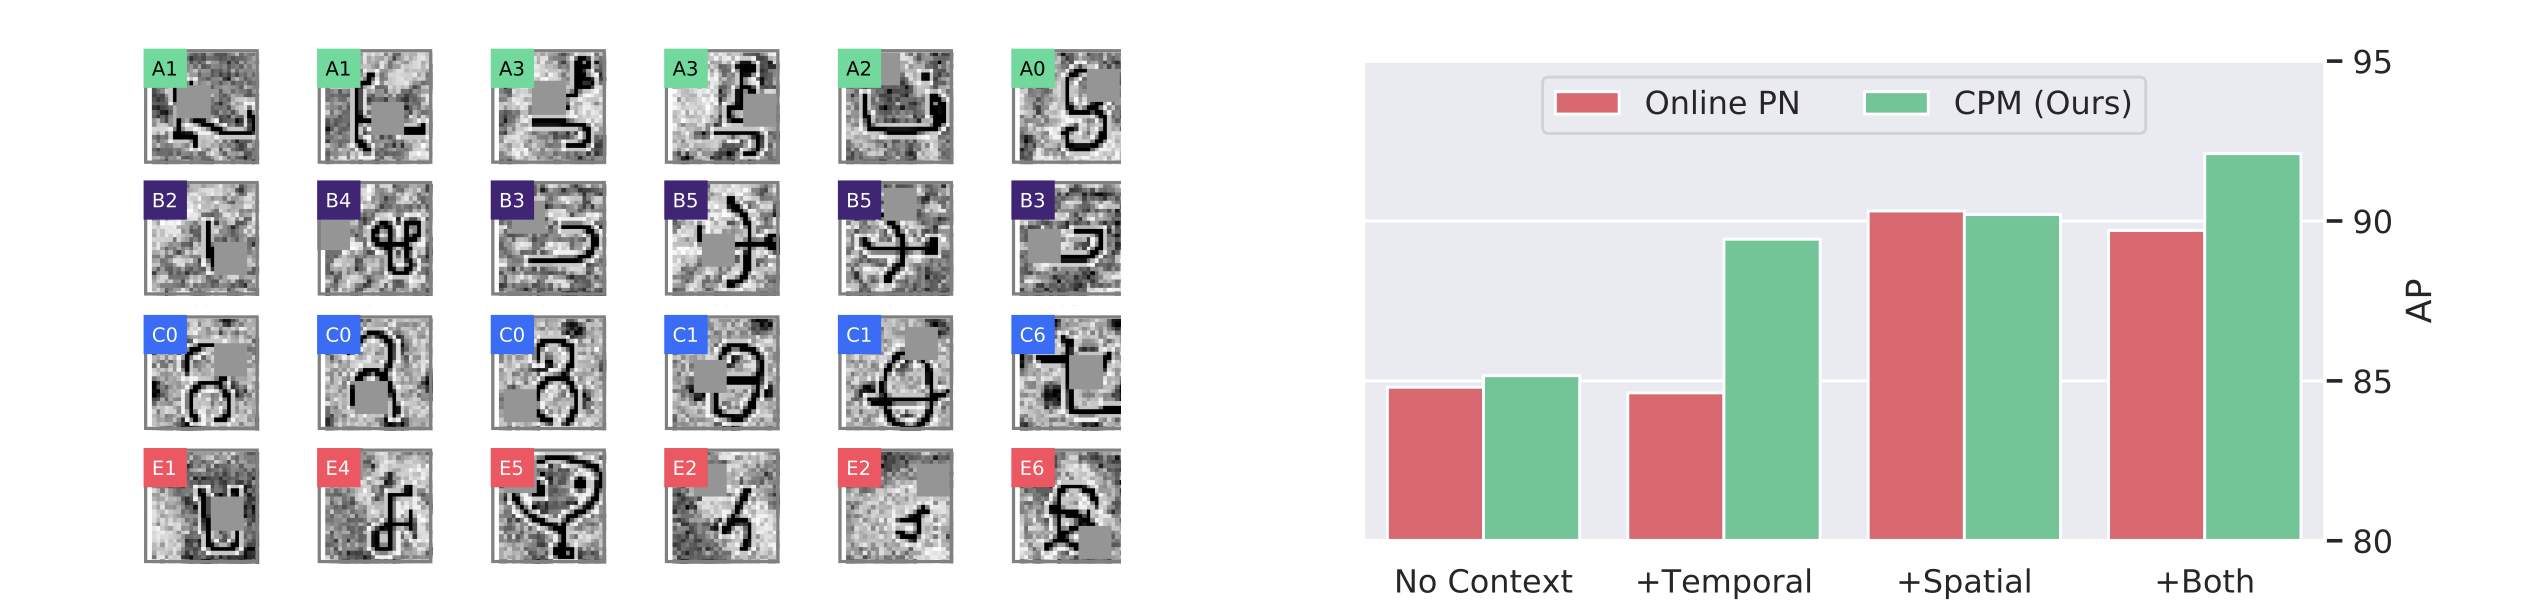
\includegraphics[width=6\linewidth]{figures/spatiotemporal_full.png}
\else
    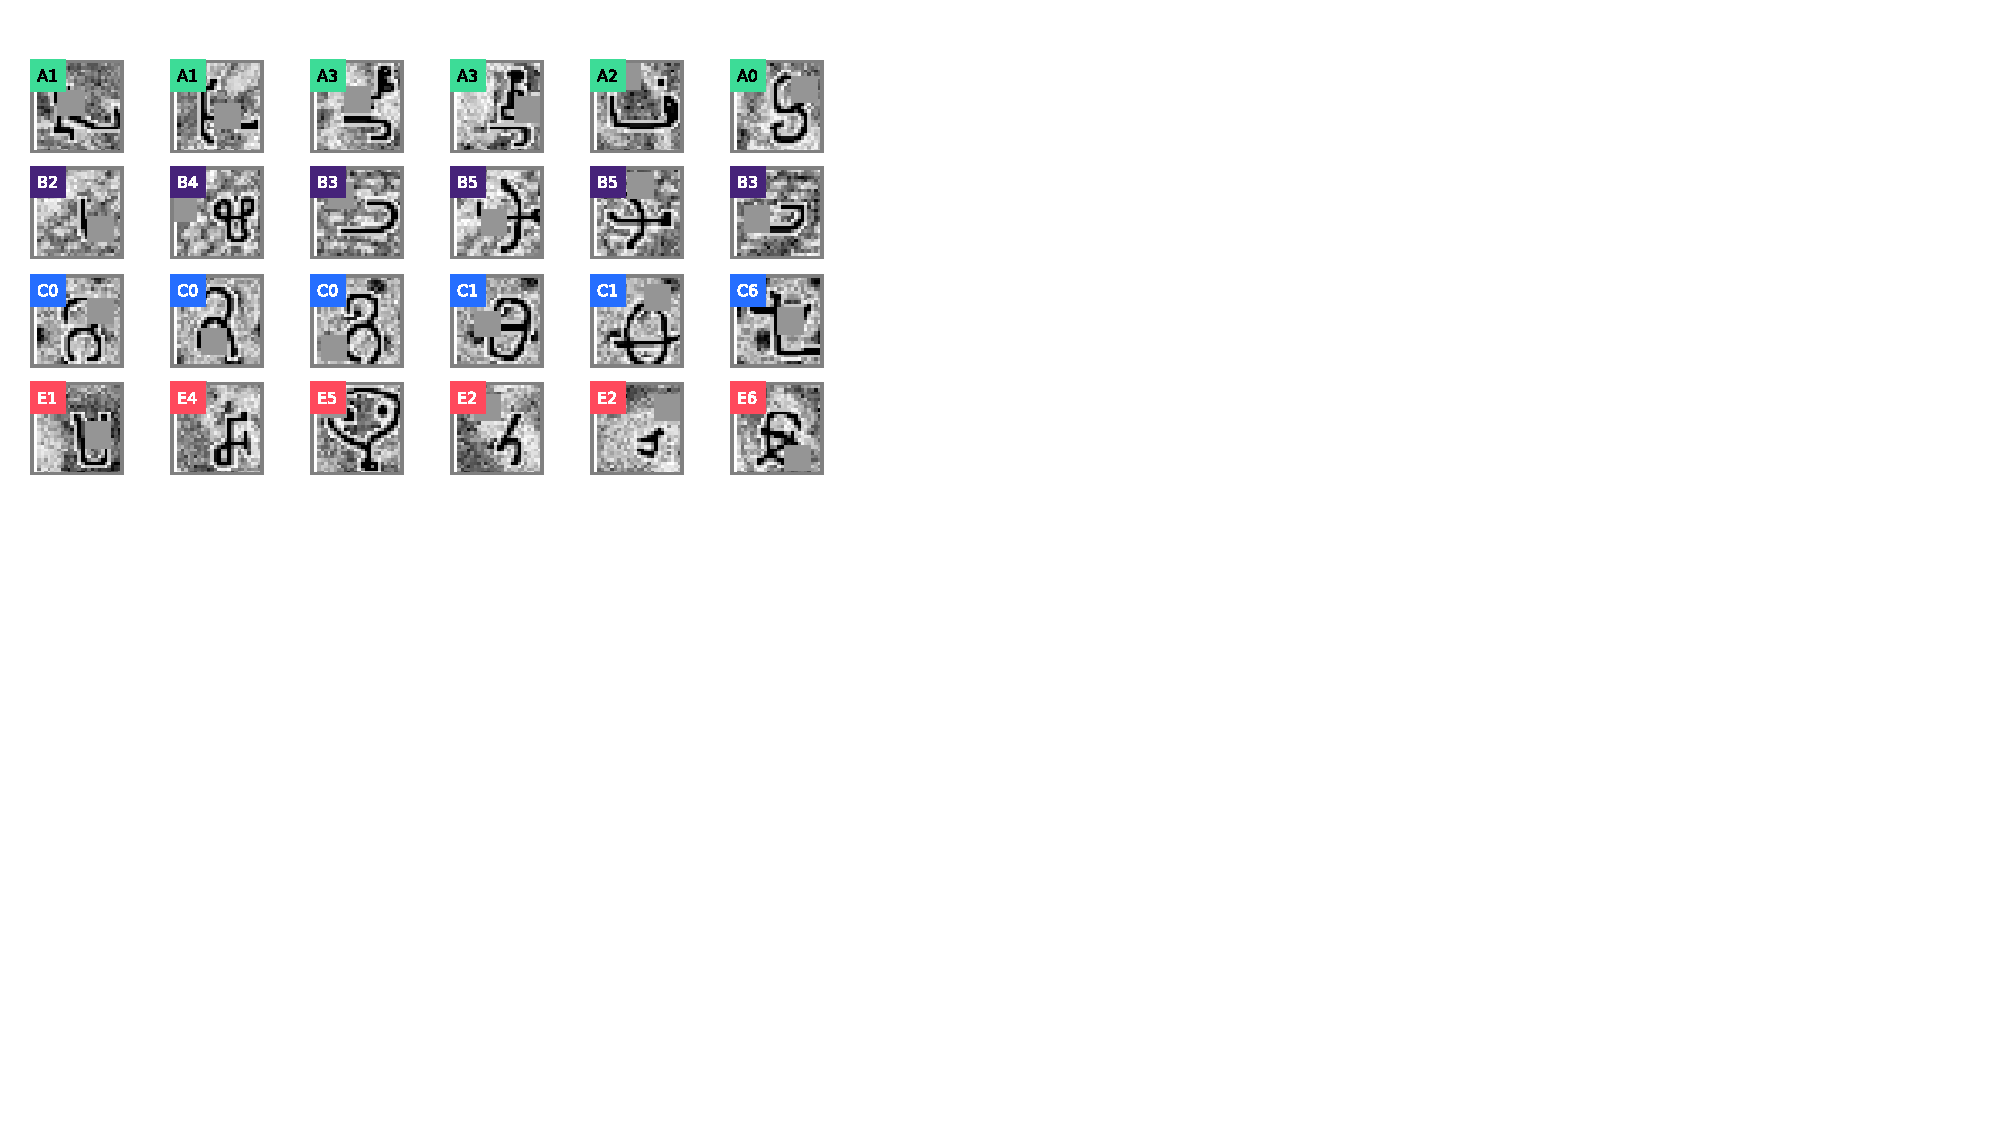
\includegraphics[height=2.8cm,trim={-2.25cm 10cm 20cm 0.5cm},clip]{figures/omniglot-texture.pdf}
    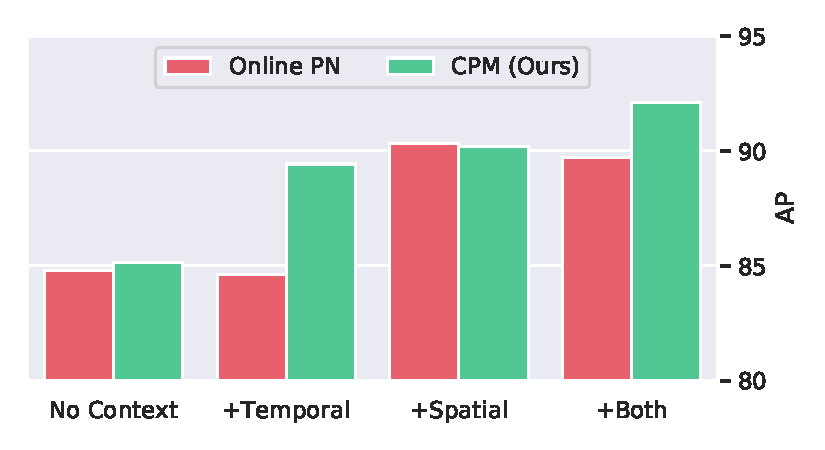
\includegraphics[height=2.8cm,trim={-2.25cm 0 0.5cm 0},clip]{figures/spatiotemporal.pdf}
\fi
\quad
\vspace{-0.2in}
\caption{\textbf{Effect of spatiotemporal context.} Spatiotemporal
context are added separately and together in \ourchar{}, by introducing texture background and
temporal correlation. \textbf{Left:} Stimuli used for spatial cue of the background environment.
\textbf{Right:} Our CPM model benefits from the presence of a temporal context
(``+Temporal'' and ``+Both'')} %, while Spatial context helps both CPM and online ProtoNet.}
\label{fig:spatiotemporal}
% \vspace{-0.1in}
\end{figure}

\vspace{-0.1in}
\iflatexml
\begin{itemize}
    \item \textbf{OML}~\citep{oml}: This is an online version of MAML~\citep{maml}. It performs one
    gradient descent step for each labeled input image, and slow weights are learned via
    backpropagation through time. On top of OML, we added an unknown predictor $\hat{u}_t = 1 -
    \max_k \hat{y}_{t,k}$ \footnote{We tried a few other ways and this is found to be the
    best.} (\textbf{OML-U}). We also found that using cosine classifier without the last layer ReLU
    is usually better than using the original dot-product classifier, and this improvement is denoted
    as \textbf{OML-U++}.
    \item \textbf{LSTM}~\citep{lstm} \& \textbf{DNC}~\citep{dnc}: We include RNN methods for
    comparison as well. Differentiable neural computer (DNC) is an improved version of memory
    augmented neural network (MANN)~\citep{mann}.
    \item \textbf{Online MatchingNet (\OnlineMatchingNet{})}~\citep{matchingnet}, 
    \textbf{IMP (\OnlineIMP{})}~\citep{imp} \&
    \textbf{ProtoNet (\OnlineProtoNet{})}~\citep{protonet}: We used\ the same negative Euclidean distance as the
    similarity function for these three metric learning based approaches.  In particular,
    MatchingNet stores all examples and performs nearest neighbor matching, which can be memory
    inefficient. Note that Online ProtoNet is a variant of our method without the contextual RNN.
\end{itemize}
\else
\begin{itemize}[leftmargin=*]
    \item \textbf{OML}~\citep{oml}: This is an online version of MAML~\citep{maml}. It performs one
    gradient descent step for each labeled input image, and slow weights are learned via
    backpropagation through time. On top of OML, we added an unknown predictor $\hat{u}_t = 1 -
    \max_k \hat{y}_{t,k}$ \footnote{We tried a few other ways and this is found to be the
    best.} (\textbf{OML-U}). We also found that using cosine classifier without the last layer ReLU
    is usually better than using the original dot-product classifier, and this improvement is denoted
    as \textbf{OML-U++}.
    \item \textbf{LSTM}~\citep{lstm} \& \textbf{DNC}~\citep{dnc}: We include RNN methods for
    comparison as well. Differentiable neural computer (DNC) is an improved version of memory
    augmented neural network (MANN)~\citep{mann}.
    \item \textbf{Online MatchingNet (\OnlineMatchingNet{})}~\citep{matchingnet}, 
    \textbf{IMP (\OnlineIMP{})}~\citep{imp} \&
    \textbf{ProtoNet (\OnlineProtoNet{})}~\citep{protonet}: We used\ the same negative Euclidean distance as the
    similarity function for these three metric learning based approaches.  In particular,
    MatchingNet stores all examples and performs nearest neighbor matching, which can be memory
    inefficient. Note that Online ProtoNet is a variant of our method without the contextual RNN.
\end{itemize}
\fi
\iflatexml
\begin{table}[t]
    \centering
    \begin{tabular}{ccccccc|cccccc}
    \toprule
    & \multicolumn{6}{c|}{\textbf{Supervised}} & \multicolumn{6}{c}{\textbf{Semi-Supervised}}\\
    Interval  &   1 - 2&      3 - 5&      6 - 10&     11 - 20&    21 - 50&    51 - 100&
                    1 - 2&      3 - 5&      6 - 10&     11 - 20&    21 - 50&    51 - 100\\
    OPN 1-Shot  &   88.8&       86.9&       85.2&       84.7&	    83.6&	    81.1&
                    90.1&       88.9&	    88.4&	    87.6&	    87.3&	    85.1\\
    CPM 1-Shot  &   \tb{96.1}&  \tb{94.0}&	\tb{93.0}&  \tb{91.6}&	\tb{88.2}&  \tb{84.6}&
                    \tb{95.9}&  \tb{93.8}&  \tb{92.8}&  \tb{91.8}&	\tb{89.4}&  \tb{85.7}\\
    OPN 3-Shot  &   97.2&	    97.1&	    96.6&	    96.7&	    \tb{96.5}&	95.3&
                    97.8&	    97.3&	    97.1&	    \tb{97.8}&	\tb{97.7}&  \tb{96.8}\\
    CPM 3-Shot  &   \tb{98.5}&	\tb{98.2}&	\tb{97.5}&	\tb{97.2}&      95.4&   \tb{95.5}&
                    \tb{98.7}&	\tb{97.5}&	\tb{97.5}&	    96.5&	    96.3&	    92.9\\
    \bottomrule
    \end{tabular}
    \caption{\textbf{Effect of forgetting over a time interval on \ourchar{}.} Average accuracy vs. the number of time steps since the model has last seen the label of a particular class.}
    \label{tab:forgetomniglot}
\end{table}
\else
\begin{table}[t]
\vspace{-0.5in}
    \centering
    \caption{\textbf{Effect of forgetting over a time interval on \ourchar{}.} Average accuracy vs. the number of time steps since the model has last seen the label of a particular class.}
    \vspace{0.1in}
    \resizebox{\textwidth}{!}{
    \begin{tabular}{ccccccc|cccccc}
    \toprule
    & \mc{6}{c}{\bf Supervised} & \mc{6}{c}{\bf Semi-Supervised}\\
    Interval  &   1 - 2&      3 - 5&      6 - 10&     11 - 20&    21 - 50&    51 - 100&
                    1 - 2&      3 - 5&      6 - 10&     11 - 20&    21 - 50&    51 - 100\\
    \midrule
    OPN 1-Shot  &   88.8&       86.9&       85.2&       84.7&	    83.6&	    81.1&
                    90.1&       88.9&	    88.4&	    87.6&	    87.3&	    85.1\\
    CPM 1-Shot  &   \bf{96.1}&  \bf{94.0}&	\bf{93.0}&	\bf{91.6}&	\bf{88.2}&  \bf{84.6}&
                    \bf{95.9}&  \bf{93.8}&  \bf{92.8}&	\bf{91.8}&	\bf{89.4}&	\bf{85.7}\\
    \midrule
    OPN 3-Shot  &   97.2&	    97.1&	    96.6&	    96.7&	    \bf{96.5}&	95.3&
                    97.8&	    97.3&	    97.1&	    \bf{97.8}&	\bf{97.7}&  \bf{96.8}\\
    CPM 3-Shot  &   \bf{98.5}&	\bf{98.2}&	\bf{97.5}&	\bf{97.2}&      95.4&  \bf{95.5}&
                    \bf{98.7}&	\bf{97.5}&	\bf{97.5}&	    96.5&	    96.3&	    92.9\\
    \bottomrule
    \end{tabular}}
    \label{tab:forgetomniglot}
\end{table}
\fi

% !TEX root = ../main.tex
\newcommand{\bgstar}{\beta_t^*, \gamma_t^*}
\newcommand{\bgw}{\beta_t^w$, $\gamma_t^w}
\newcommand{\hrnn}{\bh^{\text{RNN}}}


\iflatexml
    \begin{table}[t]
    \begin{center}
    \begin{tabular}{ccccccc}
    \toprule
    \tb{Method}                   & $\hrnn$ & $\bgstar$ & Metric $\bmm_t$ & GAU  & Val AP      \\
    \midrule                                                            
    \OnlineProtoNet{}             &         &           &                 &      & 91.22       \\
    No $\bh^{\text{RNN}}$         &         &  \yes     & \yes            &      & 92.52       \\
    $\bh^{\text{RNN}}$ only       & \yes    &           &                 &      & 93.48       \\
    No metric $\bmm_t$            & \yes    &  \yes     &                 &      & 93.61       \\
    No $\beta_t^*, \gamma_t^*$    & \yes    &           & \yes            &      & 93.98       \\
    $\bh_t = \bh_t^{\text{RNN}}$  & \yes    &  \yes     & \yes            &      & 93.70       \\
    CPM Avg. Euc                  & \yes    &  \yes     & \yes            &      & 94.08       \\
    CPM Avg. Cos                  & \yes    &  \yes     & \yes            &      & 94.57       \\
    CPM GAU Euc                   & \yes    &  \yes     & \yes            & \yes & 94.11       \\
    CPM GAU Cos                   & \yes    &  \yes     & \yes            & \yes & \tb{94.65}  \\
    \bottomrule
    \end{tabular}
    \end{center}
    \caption{Ablation of CPM architectural components on \ourchar{}}
    \label{tab:ablation} 
    \end{table}

    \begin{table}[t]
    \begin{center}
    \begin{tabular}{cccccccc}
    \toprule
    \tb{Method}         & RNN   & Prototype & $\bgw$ & GAU  & Val AP     \\
    \midrule                                                                                   
    \OnlineProtoNet{}   &       &           &        &      & 90.83      \\
    \OnlineProtoNet{}   &       &  \yes     &        &      & 89.10      \\
    \OnlineProtoNet{}   &       &  \yes     & \yes   &      & 91.22      \\
    CPM                 &       &           &        &      & 92.57      \\
    CPM                 &  \yes &           &        &      & 93.16      \\
    CPM                 &  \yes &  \yes     &        &      & 93.20      \\
    CPM                 &  \yes &  \yes     & \yes   &      & 94.08      \\
    CPM                 &  \yes &  \yes     & \yes   & \yes & \tb{94.65} \\
    \bottomrule
    \end{tabular}
    \end{center}
    \caption{Ablation of semi-supervised learning components on \ourchar{}}
    \label{tab:ablationssl}
    \end{table}
\else
    \begin{table}[t]
    \vspace{-0.1in}
    \begin{minipage}[t]{0.45\textwidth}
    \begin{small}
    \caption{Ablation of CPM architectural components on \ourchar{}}
    \begin{center}
    \label{tab:ablation}
    \resizebox{!}{1.4cm}{
    \begin{tabular}{ccccccc}
    \toprule
    \tb{Method}                   & $\hrnn$ & $\bgstar$ & Metric $\bmm_t$ & GAU  & Val AP      \\
    \midrule                                                            
    \OnlineProtoNet{}             &         &           &                 &      & 91.22       \\
    No $\bh^{\text{RNN}}$         &         &  \yes     & \yes            &      & 92.52       \\
    $\bh^{\text{RNN}}$ only       & \yes    &           &                 &      & 93.48       \\
    No metric $\bmm_t$            & \yes    &  \yes     &                 &      & 93.61       \\
    No $\beta_t^*, \gamma_t^*$    & \yes    &           & \yes            &      & 93.98       \\
    $\bh_t = \bh_t^{\text{RNN}}$  & \yes    &  \yes     & \yes            &      & 93.70       \\
    CPM Avg. Euc                  & \yes    &  \yes     & \yes            &      & 94.08       \\
    CPM Avg. Cos                  & \yes    &  \yes     & \yes            &      & 94.57       \\
    CPM GAU Euc                   & \yes    &  \yes     & \yes            & \yes & 94.11       \\
    CPM GAU Cos                   & \yes    &  \yes     & \yes            & \yes & \tb{94.65}  \\
    \bottomrule
    \end{tabular}
    }
    \end{center}
    \end{small}
    \end{minipage}
    \hfill
    \begin{minipage}[t]{0.45\textwidth}
    \caption{Ablation of semi-supervised learning components on \ourchar{}}
    \begin{small}
    \begin{center}
    \label{tab:ablationssl}
    \resizebox{!}{1.4cm}{
    \begin{tabular}{cccccccc}
    \toprule
    \tb{Method}         & RNN   & Prototype & $\bgw$ & GAU  & Val AP     \\
    \midrule                                                                                   
    \OnlineProtoNet{}   &       &           &        &      & 90.83      \\
    \OnlineProtoNet{}   &       &  \yes     &        &      & 89.10      \\
    \OnlineProtoNet{}   &       &  \yes     & \yes   &      & 91.22      \\
    CPM                 &       &           &        &      & 92.57      \\
    CPM                 &  \yes &           &        &      & 93.16      \\
    CPM                 &  \yes &  \yes     &        &      & 93.20      \\
    CPM                 &  \yes &  \yes     & \yes   &      & 94.08      \\
    CPM                 &  \yes &  \yes     & \yes   & \yes & \tb{94.65} \\
    \bottomrule
    \end{tabular}
    }
    \end{center}
    \end{small}
    \end{minipage}
    \vspace{-0.1in}
    \end{table}
 \fi


\vspace{-0.1in}
\paragraph{Main results:} Our main results are shown in Table~\ref{tab:omniglot}, 
\ref{tab:matterport} and \ref{tab:imagenet}, including both supervised and semi-supervised settings. Our approach achieves
the best performance on AP consistently across all settings. Online ProtoNet is a direct comparison
without our contextual RNN and it is clear that CPM is significantly better. Our method is slightly
worse than Online MatchingNet in terms of 3-shot accuracy on the \ourroom{} semisupervised
benchmark. This can be explained by the fact that MatchingNet stores all past seen examples, whereas
CPM only stores one prototype per class. Per timestep accuracy is plotted in
Figure~\ref{fig:acctimefull}, and the decaying accuracy is due to the increasing number of classes
over time. In \ourchar{}, CPM is able to closely match or even sometimes surpass the offline
classifier, which re-trains at each step and uses all images in a sequence except the current one. This is
reasonable as our model is able to leverage information from the current context.

\vspace{-0.1in}
\paragraph{Effect of spatiotemporal context:} To answer the question whether the gain in performance
is due to spatiotemporal reasoning, we conduct the following experiment comparing CPM with online
ProtoNet. We allow the CNN to have the ability to recognize the context in \ourchar{} by adding a
texture background image using the Kylberg texture dataset~\citep{uppsala} (see
Figure~\ref{fig:spatiotemporal} left). As a control, we can also destroy the temporal context by
shuffling all the images in a sequence. We train four different models on dataset controls with or
without the presence of spatial or temporal context, and results are shown in
Figure~\ref{fig:spatiotemporal}. First, both online ProtoNet and CPM benefit from the inclusion of a
spatial context. This is understandable as the CNN has the ability to learn spatial cues, which
re-confirms our  main hypothesis that successful inference of the current context is beneficial to
novel object recognition. Second, only our CPM model benefits from the presence of temporal context,
and it receives distinct gains from spatial and temporal contexts.

\vspace{-0.1in}
\paragraph{Effect of forgetting:} As the number of learned classes increases, we expect the average accuracy to drop. To further investigate this forgetting effect, we measure the average accuracy in terms of the number of time steps the model has last seen the label of a particular class. It is reported in Table~\ref{tab:forgetomniglot} and in Appendix~\ref{sec:additionalresults} Table~\ref{tab:forgetroom}, \ref{tab:forgetimagenet}, where we directly compare CPM and OPN to see the effect of temporal context.
CPM is significantly better than OPN on 1-shot within a short interval, which suggests that the contextual RNN 
makes the recall of the recent past much easier. On \ourimg{}, OPN eventually surpasses CPM on longer horizon, and this can be explained by the fact that OPN has more stable prototypes, whereas prototypes in CPM could potentially be affected by the fluctuation of the contextual RNN over a longer horizon.

\vspace{-0.1in}
\paragraph{Ablation studies:} We ablate each individual module we introduce. Results are shown in
Tables~\ref{tab:ablation} and~\ref{tab:ablationssl}. Table~\ref{tab:ablation} studies different ways
we use the RNN, including the context vector $\bh^{\text{RNN}}$, the predicted threshold parameters
$\beta_t^*,\gamma_t^*$, and the predicted metric scaling vector $\bmm_{t}$. Table~\ref{tab:ablationssl}
studies various ways to learn from unlabeled examples, where we separately disable the RNN update,
prototype update, and distinct write-threshold parameters $\beta^w_t, \gamma^w_t$ (vs. using
read-threshold parameters), which makes it robust to potential mistakes made in
semi-supervised learning. We verify that each component has a positive impact on the performance.

%\section{Conclusion}
\vspace{-0.1in}
Meta-learning algorithms identify the inductive bias from source tasks and make models more adaptive towards unseen novel distribution.
In this paper, we take initial steps towards characterizing the difficulty of meta-learning and understanding how these limitations present in practice. We have derived both lower bounds and upper bounds on the error of meta-learners, which are particularly relevant in the few-shot learning setting where $k$ is small. Our bounds capture key features of the meta-learning problem, such as the effect of increasing the number of shots or training tasks.
We have also identified a gap between our lower and upper bounds when there are a large number of training tasks, which we hypothesize is a limitation of the proof technique that we applied to derive the lower bounds --- suggesting an exciting direction for future research.



%\clearpage

%\section*{Broader Impact}
%Our work focuses primarily on sample complexity bounds for meta learning. It is difficult to assess the societal impact of theoretical research but our hope is to drive fundamental improvements to meta-learning and this will certainly have significant societal impact. Meta-learning researchers seek to create more general, data-efficient, and robust learning algorithms. On one hand, improved data efficiency empowers groups without access to large datasets to utilize machine learning methods; for example language models for less common written/spoken languages. But these improvements are largely applicable to other settings we may not target as researchers; such as military and surveillance applications where novel distributions and limited data are common-place.
%\bibliography{references}
%\bibliographystyle{style/icml2020}
%\clearpage

%%%%%%%%%%%%%%%%%%%%%%%%%%%%%%%%%%%%%%%%%%%%%%%%%%%%%%%%%%%%%%%%%%%%%%%%%%%%%%%
%%%%%%%%%%%%%%%%%%%%%%%%%%%%%%%%%%%%%%%%%%%%%%%%%%%%%%%%%%%%%%%%%%%%%%%%%%%%%%%

%\appendix
%\onecolumn
%% !TEX root = ../main.tex
\section{Dataset Details}
\label{app:data}

\subsection{Benchmark comparison}
We include Table~\ref{tab:benchmark} to compare existing continual and few-shot learning paradigms.

\subsection{\ourchar{} \& \ourimg{} Sampler Details}
For the \ourchar{} and the \ourimg{} experiments, we use sequences with maximum 150 images, from 5 environments. For
individual environment, we use a Chinese restaurant process to sample the class distribution. In
particular, the probability of sampling a new class is:
\begin{align}
p_\text{new} = \frac{k \alpha + \theta}{m + \theta},
\end{align}
where $k$ is the number of classes that we have already sampled in the environment, and $m$ is the
total number of instances we have in the environment. $\alpha$ is set to 0.2 and $\theta$ is set to
1.0 in all experiments.

The environment switching is implemented by a Markov switching process. At each step in the
sequence there is a constant probability $p_\text{switch}$ that switches to another environment. For
all experiments, we set $p_\text{switch}$ to 0.2. We truncate the maximum number of appearances
per class to 6. If the maximum appearance is reached, we will sample another class.

\subsection{Metrics}
\label{sec:metrics}
\paragraph{Average precision:} We chose to use AP (average precision or area under the precision-recall curve) as a way of integrating two aspects of performance:

\begin{enumerate}
    \item the binary accuracy of whether an instance belongs to a known or unknown class (KU-Assign for short), and
    \item the accuracy of assigning an instance the correct class label given it is from a known class (Class-Assign for short).
\end{enumerate}
The procedure to calculate AP is as follows. We first sort all the {KU-Assign, Class-Assign} predictions across all sequences in descending order based on KU-Assign probability, where the high ranked predictions should be known (not novel) classes. For the N top ranked instances in the sorted list, we compute:
\begin{enumerate}
    \item precision@N = correct(Class-Assign)@N / N
    \item recall@N = correct(Class-Assign)@N / K,
\end{enumerate}
where K is the true number of known instances and correct(Class-Assign)@N is the count of the number of correct class assignments among the top N. (The class assignment for an unknown instance is always incorrect.) To obtain the AP, we compute the integral of the function (y=precision@N, x=recall@N) across all N’s.

\paragraph{N-shot accuracy:} We define N-shot accuracy as the number of times an instance that has been seen N times thus far in the sequence is classified correctly. We compute the mean and standard error of this over all sequences.

\subsection{Additional \ourroom{} Statistics} 
Statistics of the \ourroom{} are included in Table~\ref{tab:dataset_stats}, in comparison to other
few-shot and continual learning datasets. Note that since \ourroom{} is collected from a simulated
environment, with 90 indoor worlds consisting of 1.2K panorama images and 1.22M video frames. The
dataset contains about 6.9K random walk sequences with a maximum of 200 frames per sequence. For
training we randomly crop 100 frames to form a training sequence. There are 7.0K unique instance
classes.

Plots of additional statistics of \ourroom{} are shown in Figure~\ref{fig:additionalstats}. In
addition to the ones shown in the main paper, instances and viewpoints also follow long tail
distributions. The number of objects in each frame follows an exponential distribution.

% !TEX root = ../main.tex
\begin{table}[t]
\iflatexml
    \begin{tabular}{ccccccc}
    \toprule
                                  & {\bf Images} & {\bf Sequences} & {\bf Classes} & {\bf Content}                  \\
    \midrule                                                                     
    Permuted MNIST~\citep{mnist}   & 60K          & -           & -          & Hand written digits          \\
    Omniglot~\citep{omniglot}      & 32.4K        & -           & 1.6K       & Hand written characters      \\
    CIFAR-100~\citep{cifar}        & 50K          & -           & 100        & Common objects               \\
    mini-ImageNet~\citep{matchingnet}& 50K        & -           & 100        & Common objects               \\
    tiered-ImageNet~\citep{fewshotssl}& 779K      & -           & 608        & Common objects               \\
    OpenLORIS  \citep{openloris}   & 98K          & -           & 69         & Small table-top obj.         \\
    CORe50  \citep{core50}         & 164.8K       & 11          & 50         & Hand-held obj.               \\
    \midrule                                                                                                          
    \ourroom{} (Ours)            & 1.22M         & 6.9K        & 7.0K       & General indoor instances     \\
    \bottomrule
    \end{tabular}
    \caption{\small Continual \& few-shot learning datasets}
    \label{tab:dataset_stats}
\else
    \vspace{-0.5in}
    \begin{center}
    \begin{small}
    \caption{\small Continual \& few-shot learning datasets}
    \label{tab:dataset_stats}
    \begin{tabular}{ccccccc}
    \toprule
                                  & {\bf Images} & {\bf Sequences} & {\bf Classes} & {\bf Content}                  \\
    \midrule                                                                     
    Permuted MNIST~\citep{mnist}   & 60K          & -           & -          & Hand written digits          \\
    Omniglot~\citep{omniglot}      & 32.4K        & -           & 1.6K       & Hand written characters      \\
    CIFAR-100~\citep{cifar}        & 50K          & -           & 100        & Common objects               \\
    mini-ImageNet~\citep{matchingnet}& 50K        & -           & 100        & Common objects               \\
    tiered-ImageNet~\citep{fewshotssl}& 779K      & -           & 608        & Common objects               \\
    OpenLORIS  \citep{openloris}   & 98K          & -           & 69         & Small table-top obj.         \\
    CORe50  \citep{core50}         & 164.8K       & 11          & 50         & Hand-held obj.               \\
    \midrule                                                                                                          
    \ourroom{} (Ours)            & 1.22M         & 6.9K        & 7.0K       & General indoor instances     \\
    \bottomrule
    \end{tabular}
    \vspace{-0.2in}
    \end{small}
    \end{center}
\fi
\end{table}


\subsection{\ourroom{} Simulator Details}
We generate our episodes with a two-stage process using two simulators -- HabitatSim~\citep{habitat}
and MatterSim~\citep{mattersim} -- because HabitatSim is based on 3D meshes and using HabitatSim
alone will result in poor image quality due to incorrect mesh reconstruction. Therefore we
sacrificed the continuous movement of agents within HabitatSim and base our environment navigation
on the discrete viewpoints in MatterSim, which is based on real panoramic images. The horizontal
field of view is set to 90 degrees for HabitatSim and 100 degrees for MatterSim, and we simulate
with\ 800$\times$600 resolution.

The first stage of generation involves randomly picking a sequence of viewpoints on the connectivity
graph within MatterSim. For each viewpoint, the agent scans the environment along the yaw and pitch
axes for a random period of time until a navigable viewpoint is within view. The time spent in a
single viewpoint follows a Gaussian distribution with mean 5.0 and standard deviation 1.0. At the
start of each new viewpoint, the agent randomly picks a direction to rotate and takes 12.5 degree
steps along the yaw axis, and with 95\% probability, a 5 degree rotation along the pitch axis is
applied in a randomly chosen direction. When a navigable viewpoint is detected, the agent will
navigate to the new viewpoint and reset the direction of scan. When multiple navigable viewpoints
are present, the agent uniformly samples one.

In the second stage, an agent in HabitatSim retraces the viewpoint path and movements of the first
stage generated by MatterSim, collecting mesh-rendered RGB and instance segmentation sensor data.
The MatterSim RGB and HabitatSim RGB images are then aligned via FLANN-based feature matching
~\citep{muja2009flann}, resulting in an alignment matrix that is used to place the MatterSim RGB and
HabitatSim instance segmentation maps into alignment. The sequence of these MatterSim RGB and
HabitatSim instance segmentation maps constitute an episode.

We keep objects of the following categories: \texttt{picture, chair, lighting, cushion, table,
plant, chest of drawers, towel, sofa, bed, appliances, stool, tv monitor, clothes, toilet,
fireplace, furniture, bathtub, gym equipment, blinds, board panel}. We initially generate 600 frames
per sequence and remove all the frames with no object. Then we store every 200 image frames into a
separate file.

During training and evaluation, each video sequence is loaded, and for each image we go through each
object present in the image. We create the attention map using the segmentation groundtruth of the
selected object. The attention map and the image together form a \textit{frame} in our model input.
For training, we randomly crop 100 frames from the sequence, and for evaluation we use the first 100
frames for deterministic results.

Please visit our released code repository to download the \ourroom{} dataset.

% !TEX root = ../main.tex
\begin{table*}[t]
\iflatexml
    \begin{tabular}{ccccccc}
    \toprule
    \mr{2}{\tb{Tasks}}                     & \tb{Few}  & \tb{Semi-sup. } & \mr{2}{\tb{Continual}} & \tb{Online} & \tb{Predict}& \tb{Soft Context}  \\
                                           & \tb{Shot} & \tb{Supp. Set}  &                        & \tb{Eval.}  & \tb{New}    & \tb{Switch}        \\
    \midrule                                                                                                                                                                          
    Incremental Learning (IL) \citep{icarl}& \xm       & \xm             & \cm                    & \hx         & \xm         & \xm                \\
    Few-shot (FSL) \citep{matchingnet}     & \cm       & \xm             & \xm                    & \xm         & \xm         & \xm                \\
    Incremental FSL \citep{attnattractor}  & \cm       & \xm             & \hx                    & \xm         & \xm         & \xm                \\
    Cls. Incremental FSL \citep{fscil}     & \cm       & \xm             & \cm                    & \hx         & \xm         & \xm                \\
    Semi-supv. FSL \citep{fewshotssl}      & \cm       & \cm             & \xm                    & \xm         & \cm         & \xm                \\
    MOCA \citep{moca}                      & \cm       & \xm             & \cm                    & \xm         & \xm         & \hx                \\
    Online Mixture \citep{onlinemixture}   & \cm       & \xm             & \cm                    & \xm         & \xm         & \hx                \\
    Online Meta \citep{oml}                & \cm       & \xm             & \cm                    & \xm         & \xm         & \xm                \\
    Continual FSL* \citep{contfsl}         & \cm       & \xm             & \cm                    & \xm         & \xm         & \xm                \\
    OSAKA* \citep{osaka}                   & \cm       & \xm             & \cm                    & \cm         & \hx         & \cm                \\
    \midrule                                                                                                                                                                                         
    OC-FSL (Ours)                          & \cm       & \cm             & \cm                    & \cm         & \cm         & \cm                \\
    \bottomrule
    \end{tabular}
    \caption{Comparison of past FSL and CL paradigms vs. our online contextualized FSL (OC-FSL). * denotes concurrent work.}
    \label{tab:benchmark}
\else
    \vspace{-0.5in}
    \caption{Comparison of past FSL and CL paradigms vs. our online contextualized FSL (OC-FSL).}
    \begin{center}
    \begin{small}
    \resizebox{\textwidth}{!}{
    \begin{tabular}{ccccccc}
    \toprule
    \mr{2}{\tb{Tasks}}                     & \tb{Few}  & \tb{Semi-sup. } & \mr{2}{\tb{Continual}} & \tb{Online} & \tb{Predict}& \tb{Soft Context}  \\
                                           & \tb{Shot} & \tb{Supp. Set}  &                        & \tb{Eval.}  & \tb{New}    & \tb{Switch}        \\
    \midrule                                                                                                                                                                          
    Incremental Learning (IL) \citep{icarl}& \xm       & \xm             & \cm                    & \hx         & \xm         & \xm                \\
    Few-shot (FSL) \citep{matchingnet}     & \cm       & \xm             & \xm                    & \xm         & \xm         & \xm                \\
    Incremental FSL \citep{attnattractor}  & \cm       & \xm             & \hx                    & \xm         & \xm         & \xm                \\
    Cls. Incremental FSL \citep{fscil}     & \cm       & \xm             & \cm                    & \hx         & \xm         & \xm                \\
    Semi-supv. FSL \citep{fewshotssl}      & \cm       & \cm             & \xm                    & \xm         & \cm         & \xm                \\
    MOCA \citep{moca}                      & \cm       & \xm             & \cm                    & \xm         & \xm         & \hx                \\
    Online Mixture \citep{onlinemixture}   & \cm       & \xm             & \cm                    & \xm         & \xm         & \hx                \\
    Online Meta \citep{oml}                & \cm       & \xm             & \cm                    & \xm         & \xm         & \xm                \\
    Continual FSL* \citep{contfsl}         & \cm       & \xm             & \cm                    & \xm         & \xm         & \xm                \\
    OSAKA* \citep{osaka}                   & \cm       & \xm             & \cm                    & \cm         & \hx         & \cm                \\
    \midrule                                                                                                                                                                                         
    OC-FSL (Ours)                          & \cm       & \cm             & \cm                    & \cm         & \cm         & \cm                \\
    \bottomrule
    \end{tabular}
    }
    \label{tab:benchmark}
    \\
    \vspace{0.05in}
    * denotes concurrent work.
    \end{small}
    \end{center}
\fi
\end{table*}

\subsection{Semi-supervised Labels:}
Here we describe how we sample the labeled vs. unlabeled flag for each example in the
semi-supervised sequences in both \ourchar{} and \ourroom{} datasets. Due to the imbalance in our
class distribution (from both the Chinese restaurant process and real data collection), directly
masking the label may bias the model to ignore the rare seen classes. Ideally, we would like to
preserve at least one labeled example for each class. Therefore, we designed the following
procedure.

First, for each class $k$, suppose $m_k$ is the number of examples in the sequence that belong to
the class. Let $\alpha$ be the target label ratio. Then the class-specific label ratio $\alpha_k$
is:
\begin{align}
\alpha_k = (1 - \alpha) \exp(-0.5 (m_k - 1)) + \alpha.
\label{eq:semisup}
\end{align}
We then for each class $k$, we sample a binary Bernoulli sequence based on $\Ber(\alpha_k)$. If a
class has all zeros in the Bernoulli sequence, we flip the flag of one of the instances to 1 to make
sure there is at least one labeled instance for each class.
For all experiments, we set $\alpha = 0.3$.

\subsection{Dataset Splits}
We include details about our dataset splits in Table~\ref{tab:omniglotsplit} and
\ref{tab:matterportsplit}.

\section{Experiment Details}
\label{app:exp}
\subsection{Network Architecture}
For the \ourchar{} experiment we used the common 4-layer CNN for few-shot learning with 64 channels
in each layer, resulting in a 64-d feature vector~\citep{protonet}. For the \ourroom{} experiment we
resize the input to 120$\times$160 and we use the ResNet-12 architecture~\citep{tadam} with
\{32,64,128,256\} channels per block. To represent the feature of the input image with an attention
mask, we concatenate the global average pooled feature with the attention ROI feature, resulting in
a 512d feature vector. For the contextual RNN, in both experiments we used an LSTM~\citep{lstm} with
a 256d hidden state. 

We use a linear layer to map from the output of the RNN to the features and control variables. We
obtain $\gamma^{r,w}$ by adding 1.0 to the linear layer output and then applying the softplus
activation. The bias units for $\beta^{r,w}$ are initialized to 10.0. We
also apply the softplus activation to $\bmm$ from the linear layer output.

% !TEX root = ../main.tex
\begin{table}[t]
\iflatexml
    \begin{tabular}{clll}
    \toprule

    \mr{11}{Train} &
    \texttt{Angelic} &
    \texttt{Grantha} &
    \texttt{N Ko}\\
    & 
    \texttt{Aurek-Besh} &
    \texttt{Japanese (hiragana)} &
    \texttt{Malay}
    \\
    & 
    \texttt{Asomtavruli} &
    \texttt{Sanskrit} &
    \texttt{Ojibwe}
    \\
    & 
    \texttt{Korean} &
    \texttt{Arcadian} &
    \texttt{Greek}
    \\
    & 
    \texttt{Alphabet of the Magi} &
    \texttt{Blackfoot} &
    \texttt{Futurama}
    \\
    & 
    \texttt{Tagalog} &
    \texttt{Anglo-Saxon Futhorc} &
    \texttt{Braille}
    \\
    & 
    \texttt{Cyrillic} &
    \texttt{Burmese} &
    \texttt{Avesta}
    \\
    & 
    \texttt{Gujarati} &
    \texttt{Ge ez} &
    \texttt{Syriac (Estrangelo)}
    \\
    & 
    \texttt{Atlantean} &
    \texttt{Japanese (katakana)} &
    \texttt{Balinese}
    \\
    & 
    \texttt{Atemayar Qelisayer} &
    \texttt{Glagolitic} &
    \texttt{Tifinagh}
    \\
    & 
    \texttt{Latin} &
    \texttt{Inuktitut} &
    \\
    \midrule
    \mr{2}{Val} &
    \texttt{Hebrew} &
    \texttt{Mkhedruli} &
    \texttt{Armenian}\\
    & 
    \texttt{Early Aramaic} &
    \texttt{Bengali} &
    \\
    \midrule

    \mr{5}{Test} & 
    \texttt{Gurmukhi} &
    \texttt{Kannada} & 
    \texttt{Keble} \\
    &
    \texttt{Malayalam} &
    \texttt{Manipuri} &
    \texttt{Mongolian} 
    \\
    &
    \texttt{Old Church Slavonic} &
    \texttt{Oriya} &
    \texttt{Syriac (Serto)} \\
    &
    \texttt{Sylheti} &
    \texttt{Tengwar} &
    \texttt{Tibetan}\\
    &
    \texttt{ULOG}
    \\
    \bottomrule
    \end{tabular}
     \caption{\textbf{Split information for {\it \ourchar{}}}. Each column is an alphabet and we include all the characters in the alphabet in the split. Rows are continuation of lines.}
    \label{tab:omniglotsplit}
\else
    \vspace{-0.5in}
     \caption{\textbf{Split information for {\it \ourchar{}}}. Each column is an alphabet and we include all the characters in the alphabet in the split. Rows are continuation of lines.}
    \begin{center}
    \begin{small}
    \label{tab:omniglotsplit}
    \begin{tabular}{clll}
    \toprule

    \mr{11}{Train} &
    \texttt{Angelic} &
    \texttt{Grantha} &
    \texttt{N Ko}\\
    & 
    \texttt{Aurek-Besh} &
    \texttt{Japanese (hiragana)} &
    \texttt{Malay}
    \\
    & 
    \texttt{Asomtavruli} &
    \texttt{Sanskrit} &
    \texttt{Ojibwe}
    \\
    & 
    \texttt{Korean} &
    \texttt{Arcadian} &
    \texttt{Greek}
    \\
    & 
    \texttt{Alphabet of the Magi} &
    \texttt{Blackfoot} &
    \texttt{Futurama}
    \\
    & 
    \texttt{Tagalog} &
    \texttt{Anglo-Saxon Futhorc} &
    \texttt{Braille}
    \\
    & 
    \texttt{Cyrillic} &
    \texttt{Burmese} &
    \texttt{Avesta}
    \\
    & 
    \texttt{Gujarati} &
    \texttt{Ge ez} &
    \texttt{Syriac (Estrangelo)}
    \\
    & 
    \texttt{Atlantean} &
    \texttt{Japanese (katakana)} &
    \texttt{Balinese}
    \\
    & 
    \texttt{Atemayar Qelisayer} &
    \texttt{Glagolitic} &
    \texttt{Tifinagh}
    \\
    & 
    \texttt{Latin} &
    \texttt{Inuktitut} &
    \\
    \midrule
    \mr{2}{Val} &
    \texttt{Hebrew} &
    \texttt{Mkhedruli} &
    \texttt{Armenian}\\
    & 
    \texttt{Early Aramaic} &
    \texttt{Bengali} &
    \\
    \midrule

    \mr{5}{Test} & 
    \texttt{Gurmukhi} &
    \texttt{Kannada} & 
    \texttt{Keble} \\
    &
    \texttt{Malayalam} &
    \texttt{Manipuri} &
    \texttt{Mongolian} 
    \\
    &
    \texttt{Old Church Slavonic} &
    \texttt{Oriya} &
    \texttt{Syriac (Serto)} \\
    &
    \texttt{Sylheti} &
    \texttt{Tengwar} &
    \texttt{Tibetan}\\
    &
    \texttt{ULOG}
    \\
    \bottomrule
    \end{tabular}
    \end{small}
    \end{center}
\fi
\end{table}

% !TEX root = ../main.tex
\iflatexml
\begin{table}[t]
\begin{tabular}{cc}
\toprule
\mr{12}{Train} &
\texttt{
r1Q1Z4BcV1o
JmbYfDe2QKZ
29hnd4uzFmX
ULsKaCPVFJR
E9uDoFAP3SH
}\\
&
\texttt{
8WUmhLawc2A
Uxmj2M2itWa
mJXqzFtmKg4
V2XKFyX4ASd
EU6Fwq7SyZv
}\\
&
\texttt{
gYvKGZ5eRqb
gxdoqLR6rwA
YFuZgdQ5vWj
gTV8FGcVJC9
sT4fr6TAbpF
}\\
&
\texttt{
VVfe2KiqLaN
fzynW3qQPVF
WYY7iVyf5p8
VFuaQ6m2Qom
YmJkqBEsHnH
}\\
&
\texttt{
2t7WUuJeko7
pLe4wQe7qrG
cV4RVeZvu5T
XcA2TqTSSAj
ur6pFq6Qu1A
}\\
&
\texttt{
1pXnuDYAj8r
b8cTxDM8gDG
x8F5xyUWy9e
X7HyMhZNoso
aayBHfsNo7d
}\\
&
\texttt{
TbHJrupSAjP
sKLMLpTHeUy
2azQ1b91cZZ
2n8kARJN3HM
Vvot9Ly1tCj
}\\
&
\texttt{
S9hNv5qa7GM
EDJbREhghzL
qoiz87JEwZ2
q9vSo1VnCiC
Vt2qJdWjCF2
}\\
&
\texttt{
VzqfbhrpDEA
D7G3Y4RVNrH
ZMojNkEp431
uNb9QFRL6hY
5LpN3gDmAk7
}\\
&
\texttt{
rqfALeAoiTq
e9zR4mvMWw7
yqstnuAEVhm
zsNo4HB9uLZ
JF19kD82Mey
}\\
&
\texttt{
759xd9YjKW5
wc2JMjhGNzB
rPc6DW4iMge
jh4fc5c5qoQ
HxpKQynjfin
}\\
&
\texttt{
GdvgFV5R1Z5
kEZ7cmS4wCh
vyrNrziPKCB
D7N2EKCX4Sj
PX4nDJXEHrG
}\\

\midrule

\mr{2}{Val} &
\texttt{
s8pcmisQ38h
dhjEzFoUFzH
RPmz2sHmrrY
1LXtFkjw3qL
8194nk5LbLH
}\\
&
\texttt{
jtcxE69GiFV
QUCTc6BB5sX
p5wJjkQkbXX
JeFG25nYj2p
82sE5b5pLXE
}\\
\midrule

\mr{4}{Test} & 
\texttt{
oLBMNvg9in8
r47D5H71a5s
Z6MFQCViBuw
YVUC4YcDtcY
pRbA3pwrgk9
}\\
&
\texttt{
SN83YJsR3w2
gZ6f7yhEvPG
ac26ZMwG7aT
7y3sRwLe3Va
B6ByNegPMKs
}\\
&
\texttt{
UwV83HsGsw3
VLzqgDo317F
17DRP5sb8fy
pa4otMbVnkk
5ZKStnWn8Zo
}\\
&
\texttt{
PuKPg4mmafe
Pm6F8kyY3z2
i5noydFURQK
ARNzJeq3xxb
5q7pvUzZiYa
}\\
\bottomrule
\end{tabular}
\caption{\textbf{Split information for {\it \ourroom{}}}. Each column is the ID of an indoor world. Rows are continuation of the lines.}
\label{tab:matterportsplit}
\end{table}

\begin{table}[t]
\begin{tabular}{cccc}
\toprule
Split & Worlds & Sequences & Frames \\
\midrule
Train & 60     & 4,699      &   823,444     \\
Val   & 20     &  725         &  125,823  \\
Test  & 10     &  1,547      &  271,335      \\
\midrule
Total & 90     & 6,971   & 1,220,602 \\
\bottomrule
\end{tabular}
\caption{{\it \ourroom{}} dataset split size}
\label{tab:matterportsplitsize}
\end{table}
\else
    \begin{table}[t]
    \caption{\textbf{Split information for {\it \ourroom{}}}. Each column is the ID of an indoor world. Rows are continuation of the lines.}
    \label{tab:matterportsplit}
    % \vspace{-0.5in}
    \begin{center}
    \begin{small}
    \begin{tabular}{cc}
    \toprule
    \mr{12}{Train} &
    \texttt{
    r1Q1Z4BcV1o
    JmbYfDe2QKZ
    29hnd4uzFmX
    ULsKaCPVFJR
    E9uDoFAP3SH
    }\\
    &
    \texttt{
    8WUmhLawc2A
    Uxmj2M2itWa
    mJXqzFtmKg4
    V2XKFyX4ASd
    EU6Fwq7SyZv
    }\\
    &
    \texttt{
    gYvKGZ5eRqb
    gxdoqLR6rwA
    YFuZgdQ5vWj
    gTV8FGcVJC9
    sT4fr6TAbpF
    }\\
    &
    \texttt{
    VVfe2KiqLaN
    fzynW3qQPVF
    WYY7iVyf5p8
    VFuaQ6m2Qom
    YmJkqBEsHnH
    }\\
    &
    \texttt{
    2t7WUuJeko7
    pLe4wQe7qrG
    cV4RVeZvu5T
    XcA2TqTSSAj
    ur6pFq6Qu1A
    }\\
    &
    \texttt{
    1pXnuDYAj8r
    b8cTxDM8gDG
    x8F5xyUWy9e
    X7HyMhZNoso
    aayBHfsNo7d
    }\\
    &
    \texttt{
    TbHJrupSAjP
    sKLMLpTHeUy
    2azQ1b91cZZ
    2n8kARJN3HM
    Vvot9Ly1tCj
    }\\
    &
    \texttt{
    S9hNv5qa7GM
    EDJbREhghzL
    qoiz87JEwZ2
    q9vSo1VnCiC
    Vt2qJdWjCF2
    }\\
    &
    \texttt{
    VzqfbhrpDEA
    D7G3Y4RVNrH
    ZMojNkEp431
    uNb9QFRL6hY
    5LpN3gDmAk7
    }\\
    &
    \texttt{
    rqfALeAoiTq
    e9zR4mvMWw7
    yqstnuAEVhm
    zsNo4HB9uLZ
    JF19kD82Mey
    }\\
    &
    \texttt{
    759xd9YjKW5
    wc2JMjhGNzB
    rPc6DW4iMge
    jh4fc5c5qoQ
    HxpKQynjfin
    }\\
    &
    \texttt{
    GdvgFV5R1Z5
    kEZ7cmS4wCh
    vyrNrziPKCB
    D7N2EKCX4Sj
    PX4nDJXEHrG
    }\\

    \midrule

    \mr{2}{Val} &
    \texttt{
    s8pcmisQ38h
    dhjEzFoUFzH
    RPmz2sHmrrY
    1LXtFkjw3qL
    8194nk5LbLH
    }\\
    &
    \texttt{
    jtcxE69GiFV
    QUCTc6BB5sX
    p5wJjkQkbXX
    JeFG25nYj2p
    82sE5b5pLXE
    }\\
    \midrule

    \mr{4}{Test} & 
    \texttt{
    oLBMNvg9in8
    r47D5H71a5s
    Z6MFQCViBuw
    YVUC4YcDtcY
    pRbA3pwrgk9
    }\\
    &
    \texttt{
    SN83YJsR3w2
    gZ6f7yhEvPG
    ac26ZMwG7aT
    7y3sRwLe3Va
    B6ByNegPMKs
    }\\
    &
    \texttt{
    UwV83HsGsw3
    VLzqgDo317F
    17DRP5sb8fy
    pa4otMbVnkk
    5ZKStnWn8Zo
    }\\
    &
    \texttt{
    PuKPg4mmafe
    Pm6F8kyY3z2
    i5noydFURQK
    ARNzJeq3xxb
    5q7pvUzZiYa
    }\\
    \bottomrule
    \end{tabular}
    \end{small}
    \end{center}
    \end{table}

    \begin{table}[t]
    \vspace{-0.5in}
    \caption{{\it \ourroom{}} dataset split size}
    \label{tab:matterportsplitsize}
    \begin{center}
    \begin{small}
    \begin{tabular}{cccc}
    \toprule
    Split & Worlds & Sequences & Frames \\
    \midrule
    Train & 60     & 4,699      &   823,444     \\
    Val   & 20     &  725         &  125,823  \\
    Test  & 10     &  1,547      &  271,335      \\
    \midrule
    Total & 90     & 6,971   & 1,220,602 \\
    \bottomrule
    \end{tabular}
    \end{small}
    \end{center}
    \end{table}
\fi


\begin{figure}[t]
\vspace{-0.2in}
\centering
\iflatexml
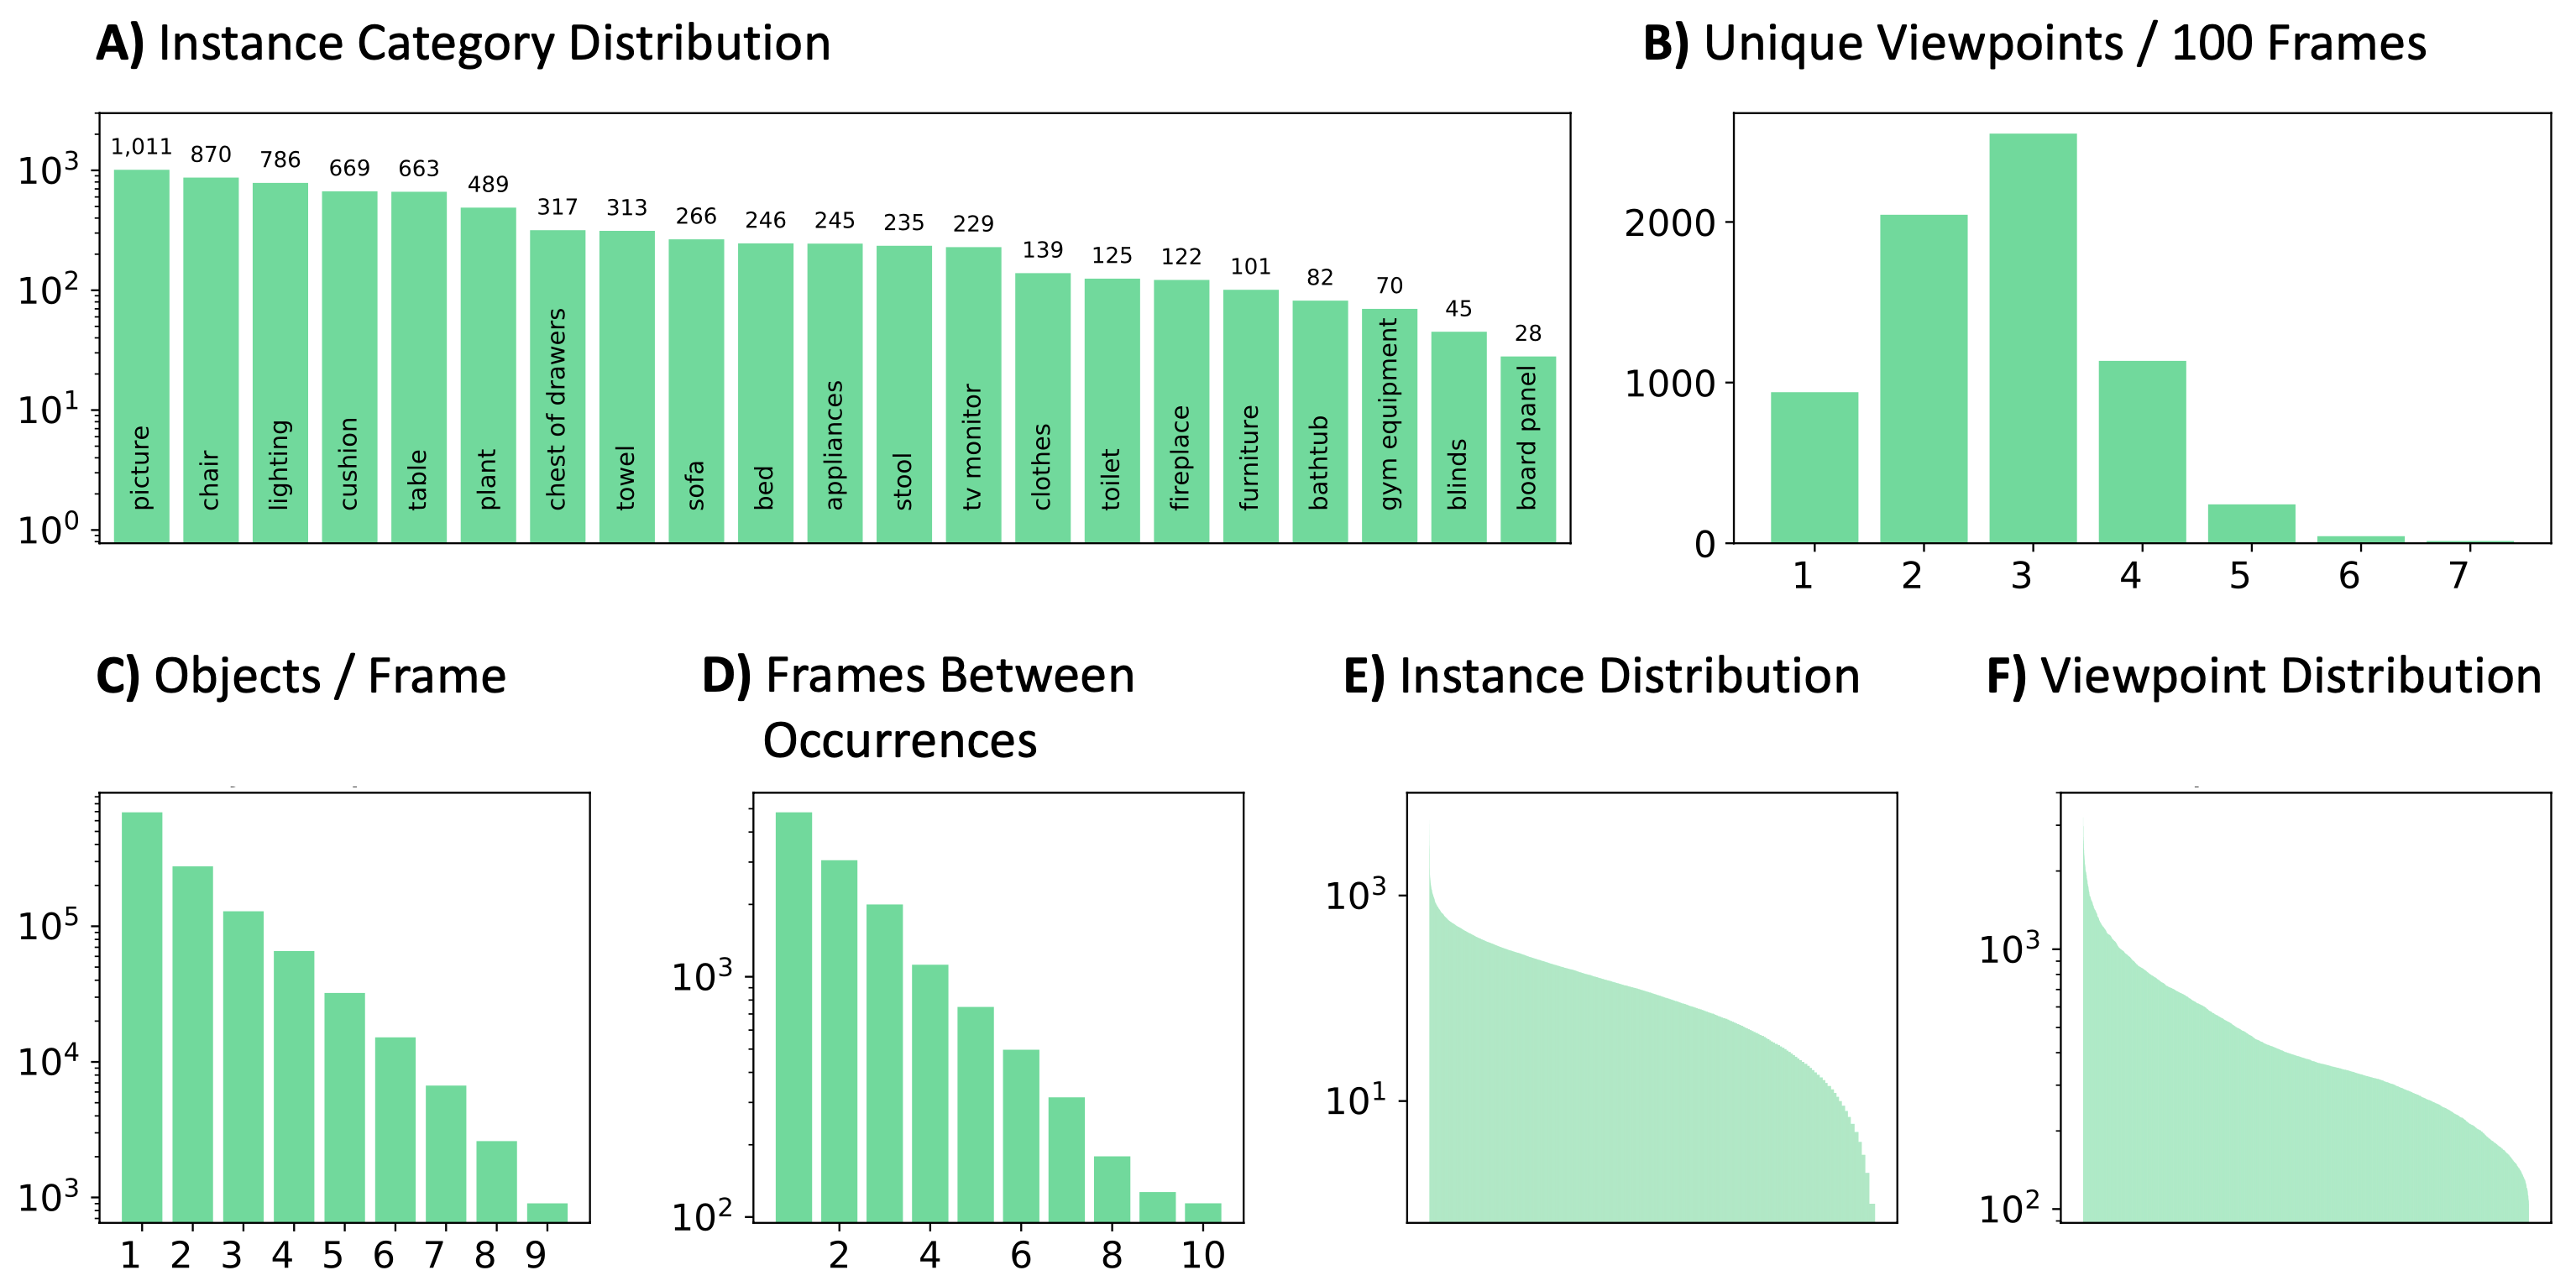
\includegraphics[width=6\textwidth]{figures/statsfull.png}
\else
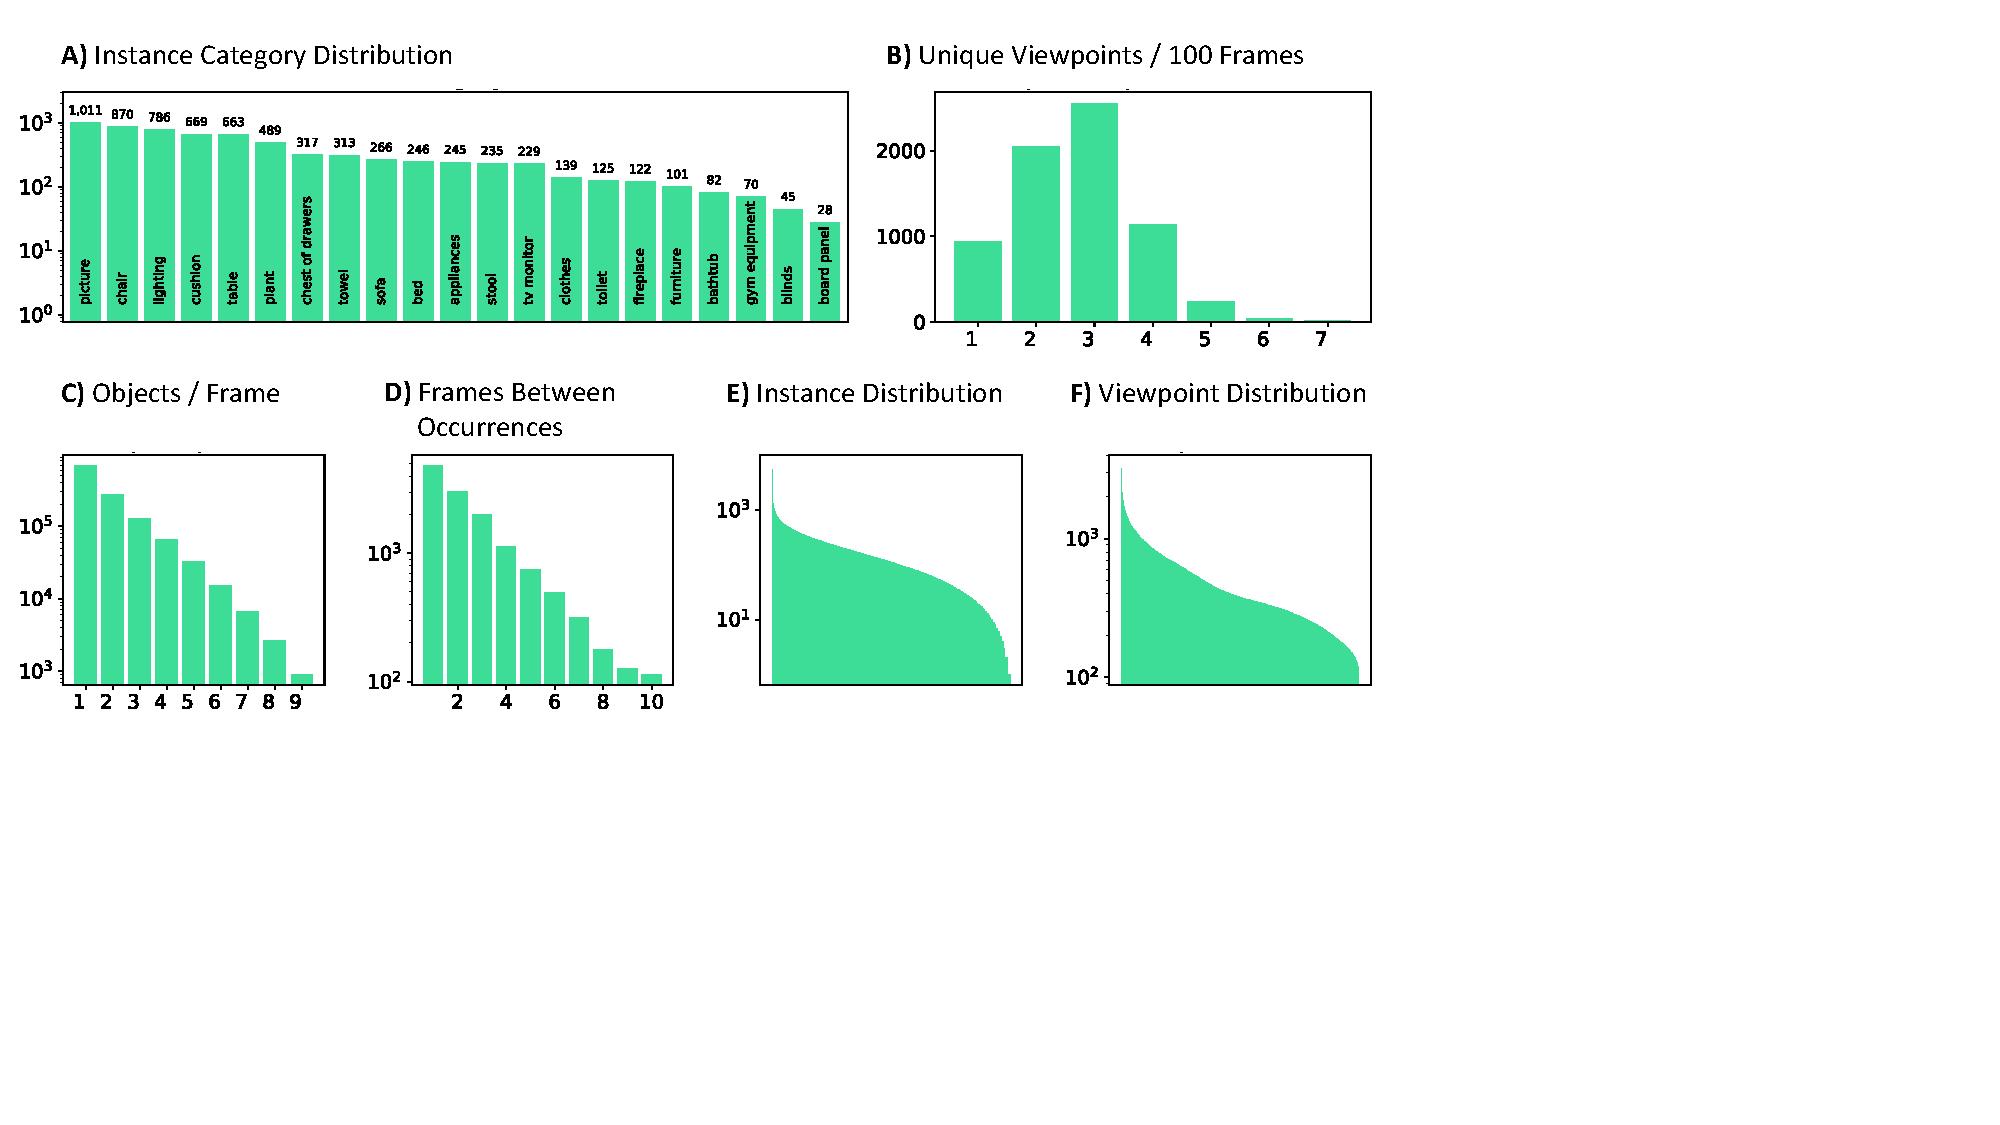
\includegraphics[width=0.9\textwidth,trim={0cm 7cm 10.2cm 0cm},clip]{figures/statsfull.pdf}
\fi
\caption{Additional statistics about our \ourroom{} dataset.}
\label{fig:additionalstats}
\end{figure}


\subsection{Training Procedure}
We use the Adam optimizer~\citep{adam} for all of our experiments, with a gradient cap of 5.0. For
\ourchar{} we train the network for 40k steps with a batch size 32 and maximum sequence length 150
across 2 GPUs and an initial learning rate 2e-3 decayed by 0.1$\times$ at 20k and 30k steps. For
\ourroom{} we train for 20k steps with a batch size 8 and maximum sequence length 100 across 4 GPUs
and an initial learning rate 1e-3 decayed by 0.1$\times$ at 8k and 16k steps. We use the BCE coefficient
$\lambda=1$  for all experiments. In semi-supervised experiments, around 30\% examples are labeled when the number of examples grows large ($\alpha = 0.3$, see Equation~\ref{eq:semisup}). Early stopping is used in \ourroom{} experiments
where the checkpoint with the highest validation AP score is chosen.
For \ourroom{}, we sample Bernoulli sequences on unlabeled inputs to 
gradually allow semi-supervised writing to the prototype memory and we find it helps training stability. The probability starts with 0.0 and increase by 0.2 every 2000 training steps until reaching 1.0.

\subsection{Data Augmentation}
For \ourchar{}, we pad the 28$\times$28 image to 32$\times$32 and then apply random cropping.

For \ourroom{}, we apply random cropping in the time dimension to get a chunk of 100 frames per
input example. We also apply random dropping of 5\% of the frames. We pad the 120$\times$160 images
to 126 $\times$ 168 and apply random cropping in each image frame. We also randomly flip the order
of the sequence (going forward or backward).


\subsection{Spatiotemporal context experiment details}
We use the Kylberg texture dataset~\citep{uppsala} without rotations. Texture classes are split into train, val, and test, defined in Table~\ref{tab:uppsalasplit}. We resize all images first to 256$\times$256. For each Omniglot image, a 28$\times$28 patch is randomly cropped from a texture image to serve as background. Random Gaussian noises with mean zero and standard deviation 0.1 are added to the background images.

For spatial background experiments, we added an additional learnable network of the same size as the main network to take the background image as input, and output the same sized embedding vector. This embedding vector is further concatenated with the main embedding vector to form the final embedding of the input. We also found that using spatially overlayed images with a single CNN can achieve similar performance as well. The final numbers are reported using the concatenation approach since it is less prone to overlay noises and is more similar to the implementation we use in the RoamingRooms experiments.

% !TEX root = ../supp.tex
\iflatexml
    \begin{table}[t]
    \begin{tabular}{clllll}
    \toprule

    \mr{3}{Train} &
    \texttt{blanket2} &
    \texttt{ceiling2} &
    \texttt{floor2} &
    \texttt{grass1} &
    \texttt{linseeds1} \\
    &
    \texttt{pearlsugar1} &
    \texttt{rice2} &
    \texttt{scarf2} &
    \texttt{screen1} &
    \texttt{seat2} \\
    &
    \texttt{sesameseeds1} &
    \texttt{stone1} & 
    \texttt{stoneslab1} & &
    \\
    \midrule

    \mr{2}{Val} &
    \texttt{blanket1} &
    \texttt{canvas1} &
    \texttt{ceiling1} & 
    \texttt{floor1} &
    \texttt{scarf1} \\
    &
    \texttt{rice1} &
    \texttt{stone2} & & & \\
    \midrule
    \mr{2}{Test} & 
    \texttt{wall1} &
    \texttt{lentils1} & 
    \texttt{cushion1} &
    \texttt{rug1} &
    \texttt{sand1} \\
    &
    \texttt{oatmeal1} &
    \texttt{stone3} &
    \texttt{seat1} & & \\
    \bottomrule
    \end{tabular}
    \caption{\textbf{Split information for the Kylberg texture dataset}. Each column is an texture type. Rows are continuation of lines.}
    \label{tab:uppsalasplit}
    \end{table}
\else
    \begin{table}[t]
    \vspace{-0.5in}
    \caption{\textbf{Split information for the Kylberg texture dataset}. Each column is an texture type. Rows are continuation of lines.}
    \label{tab:uppsalasplit}
    \begin{center}
    \begin{small}
    \begin{tabular}{clllll}
    \toprule

    \mr{3}{Train} &
    \texttt{blanket2} &
    \texttt{ceiling2} &
    \texttt{floor2} &
    \texttt{grass1} &
    \texttt{linseeds1} \\
    &
    \texttt{pearlsugar1} &
    \texttt{rice2} &
    \texttt{scarf2} &
    \texttt{screen1} &
    \texttt{seat2} \\
    &
    \texttt{sesameseeds1} &
    \texttt{stone1} & 
    \texttt{stoneslab1} & &
    \\
    \midrule

    \mr{2}{Val} &
    \texttt{blanket1} &
    \texttt{canvas1} &
    \texttt{ceiling1} & 
    \texttt{floor1} &
    \texttt{scarf1} \\
    &
    \texttt{rice1} &
    \texttt{stone2} & & & \\
    \midrule
    \mr{2}{Test} & 
    \texttt{wall1} &
    \texttt{lentils1} & 
    \texttt{cushion1} &
    \texttt{rug1} &
    \texttt{sand1} \\
    &
    \texttt{oatmeal1} &
    \texttt{stone3} &
    \texttt{seat1} & & \\
    \bottomrule
    \end{tabular}
    \end{small}
    \end{center}
    \end{table}
 \fi


\subsection{Baseline implementation details}
\paragraph{Online meta-learning (OML):} The OML  model performs one gradient descent step for each
input. In order for the model to predict unknown, we use the probability output from the softmax
layer summing across the unused units. For example, if the softmax layer has 40 units and we have
only seen 5 classes so far, then we sum the probability from the 6th to the last units. This summed
probability is separately trained with a binary cross entropy, same as in Equation~\ref{eq:loss}.

The inner learning rate is set to 1e-2 and we truncate the number of unrolled gradient descent steps
to 5/20 (\ourchar{}/\ourroom{}), in order to make the computation feasible. For \ourchar{}, the
network is trained with a batch size 32 across 2 GPUs, for a total of 20k steps, with an initial
learning rate 2e-3 decayed by 0.1 at 10k and 16.7k steps. For \ourroom{}, the network is trained
with a batch size 8 across 4 GPUs, for a total of 16k steps, with an initial learning rate 1e-3
decayed by 0.1 at 6.4k and 12.8k steps.

\paragraph{Long short-term memory (LSTM):} We apply a stacked two layer LSTM with 256 hidden
dimensions. Inputs are $\bh_t^{\text{CNN}}$ concatenated with the label one-hot vector. If an
example is unlabeled, then the label vector is all-zero. We directly apply a linear layer on top of
the LSTM to map the LSTM memory output into classification logits, and the last logit is the binary
classification logit reserved for unknown. The training procedure is the same as our CPM model.

\paragraph{Differentiable neural computer (DNC):} In order to make the DNC model work properly, we
found that it is sometimes helpful to pretrain the CNN weights. Simply initializing from scratch and
train CNN+DNC end-to-end sometimes results in poor performance. We hypothesize that the attention
structure in the DNC model is detrimental to representation learning. Therefore, for \ourchar{}
experiments, we use pretrained ProtoNet weights for solving 1-shot 5-way episodes to initialize the
CNN, and we keep finetuning the CNN weights with 10\% of the full learning rate. For \ourroom{}
experiments, we train the full model end-to-end from scratch.

The DNC is also modified so that it is more effective using the label information from the input. In
the original MANN paper~\citep{mann} for one-shot learning, the input features $\bh_t^{\text{CNN}}$
and the label one-hot ID are simply concatenated to feed into the LSTM controller of MANN. We find
that it is beneficial to directly add label one-hot vector as an input to the write head that
generates the write attention and the write content.  Similar to the LSTM model, the memory readout is also sent to a
linear layer in order to get the final classification logits, and the last logit is the binary
classification logit reserved for the unknowns. Finally we remove the linkage prediction part of the DNC
due to training instability.

The controller LSTM has 256 hidden dimensions, and the memory has 64 slots each with 64 dimensions.
There are 4 read heads and 4 write heads. The training procedure is the same as CPM.

\paragraph{Online ProtoNet:} Online ProtoNet is our modification of the original
ProtoNet~\citep{protonet}. It is similar to our CPM model without the contextual RNN. The feature
from the CNN is directly written to the prototype memory. In addition, we do not predict the control
hyperparameters $\beta^{\{r,w\}}_t,\gamma^{\{r,w\}}_t$ from the RNN and they are learned as regular parameters. The training procedure is the same as CPM.

\paragraph{Online MatchingNet:} Online MatchingNet is our modification of the original
MatchingNet~\citep{matchingnet}. We do not consider the context embedding in the MatchingNet paper
since it was originally designed for the entire episode using an attentional RNN encoder. It is
similar to online ProtoNet but instead of doing online averaging, it directly stores each example
and its class. Since it is an example-based storage, we did not extend it to learn from
unlabeled examples, and all unlabeled examples are skipped. We use a similar decision rule to
determine whether an example belongs to a known cluster by looking at the distance to the nearest
exemplar stored in the memory, shifted by $\beta$ and scaled by $1/\gamma$. Note that online
MatchingNet is not efficient at memory storage since it scales with the number of steps in the
sequence. In addition, we use the negative Euclidean distance as the similarity function. The training
procedure is the same as CPM.

\paragraph{Online infinite mixture prototypes (IMP):} Online IMP is proposed as a mix of prototype and example-based storage by allowing a class to have multiple clusters. If an
example is classified as unknown or it is unlabeled, we will assign its cluster based on our
prediction, which either assigns it to one of the existing clusters or creates a new cluster,
depending on its distance to the nearest cluster. If a cluster with an unknown label later is
assigned with an example with a known class, then the cluster label will also be updated. We use the same
decision rule as online ProtoNet to determine whether an example belongs to a known cluster by
looking at the distance to the nearest cluster, shifted by $\beta$ and scaled by $1/\gamma$. As
described above, online IMP has the capability of learning from unlabeled examples, unlike online
MatchingNet. However similar to online MatchingNet, online IMP is also not efficient at memory
storage since in the worst case it also scales with the number of steps in the sequence. Again, the
training procedure is the same as CPM.

\section{Additional Experimental Results}
\label{sec:additionalresults}
\subsection{Effect of Forgetting}
We report the effect of forgetting of \ourroom{} and \ourimg{} in Table~\ref{tab:forgetroom} and \ref{tab:forgetimagenet}.
\iflatexml
\begin{table}[t]
    \centering
    \begin{tabular}{ccccccc|cccccc}
    \toprule
    & \mc{6}{c|}{\textbf{Supervised}} & \mc{6}{c}{\textbf{Semi-Supervised}}\\
                &   1 - 2&      3 - 5&      6 - 10&     11 - 20&    21 - 50&    51 - 100&
                    1 - 2&      3 - 5&      6 - 10&     11 - 20&    21 - 50&    51 - 100\\
    OPN 1-Shot  &   93.5&   	89.3&	    79.4&	    67.2&	    60.3&	    60.1&
                    86.5&	    83.6&	    76.3&	    68.4&	    64.7&	    61.5\\
    CPM 1-Shot  &   \bf{95.7}&	\bf{92.2}&  \bf{85.7}&	\bf{75.2}&	\bf{70.0}&  \bf{66.4}&
                    \bf{91.0}&	\bf{88.7}&	\bf{82.9}&	\bf{77.0}&  \bf{72.2}&	\bf{66.5}\\
    OPN 3-Shot  &   95.1&	    91.8&	    85.6&   	78.2&	    74.6&	    73.8&
                    92.6&       88.0&	    85.1&	    81.1&	    80.6&	    76.7\\
    CPM 3-Shot  &   \bf{96.1}&	\bf{93.8}&	\bf{87.7}&	\bf{81.4}&  \bf{79.1}&	\bf{78.2}&
                    \bf{94.8}&  \bf{91.0}&	\bf{86.9}&	\bf{83.1}&	\bf{82.7}&  \bf{79.2}\\
    \bottomrule
    \end{tabular}
    \caption{\textbf{Effect of forgetting over a time interval on \ourroom{}.} Average accuracy vs. the number of time steps since the model has last seen the label of a particular class.}
    \label{tab:forgetroom}
\end{table}

\begin{table}[t]
    \centering
    \begin{tabular}{ccccccc|cccccc}
    \toprule
    & \mc{6}{c|}{\bf Supervised} & \mc{6}{c}{\bf Semi-Supervised}\\
                &   1 - 2&      3 - 5&      6 - 10&     11 - 20&    21 - 50&    51 - 100&
                    1 - 2&      3 - 5&      6 - 10&     11 - 20&    21 - 50&    51 - 100\\
    OPN 1-Shot  &   40.8&	35.9&	33.0&	\bf{30.7}&	\bf{27.0}&	\bf{21.4}&
                    40.5&	37.7&	35.9&	\bf{33.7}&	\bf{31.5}&	\bf{28.4}\\
    CPM 1-Shot  &   \bf{67.5}&	\bf{52.9}&	\bf{35.5}&	24.2&	18.3&	13.8&
                    \bf{60.4}&	\bf{51.3}&	\bf{39.5}&	26.6&	21.8&	15.4\\
    OPN 3-Shot  &   52.5&	50.3&	\bf{48.8}&	\bf{47.2}&	\bf{44.4}&	\bf{42.3}&
                    57.6&	55.1&	\bf{54.6}&	\bf{52.3}&	\bf{52.1}&	\bf{49.5}\\
    CPM 3-Shot  &   \bf{77.8}&	\bf{64.5}&	46.6&	32.9&	24.7&	17.9&
                    \bf{76.1}&	\bf{61.8}&	48.6&	30.5&	24.1&	15.6\\
    \bottomrule
    \end{tabular}
    \caption{\textbf{Effect of forgetting over a time interval on \ourimg{}.} Average accuracy vs. the number of time steps since the model has last seen the label of a particular class.}
    \label{tab:forgetimagenet}
\end{table}

\else
\begin{table}[t]
\vspace{-0.5in}
    \centering
    \caption{\textbf{Effect of forgetting over a time interval on \ourroom{}.} Average accuracy vs. the number of time steps since the model has last seen the label of a particular class.}
    
    \resizebox{\textwidth}{!}{
    \begin{tabular}{ccccccc|cccccc}
    \toprule
    & \mc{6}{c}{\bf Supervised} & \mc{6}{c}{\bf Semi-Supervised}\\
                &   1 - 2&      3 - 5&      6 - 10&     11 - 20&    21 - 50&    51 - 100&
                    1 - 2&      3 - 5&      6 - 10&     11 - 20&    21 - 50&    51 - 100\\
    \midrule
    OPN 1-Shot  &   93.5&   	89.3&	    79.4&	    67.2&	    60.3&	    60.1&
                    86.5&	    83.6&	    76.3&	    68.4&	    64.7&	    61.5\\
    CPM 1-Shot  &   \bf{95.7}&	\bf{92.2}&  \bf{85.7}&	\bf{75.2}&	\bf{70.0}&  \bf{66.4}&
                    \bf{91.0}&	\bf{88.7}&	\bf{82.9}&	\bf{77.0}&  \bf{72.2}&	\bf{66.5}\\
    \midrule
    OPN 3-Shot  &   95.1&	    91.8&	    85.6&   	78.2&	    74.6&	    73.8&
                    92.6&       88.0&	    85.1&	    81.1&	    80.6&	    76.7\\
    CPM 3-Shot  &   \bf{96.1}&	\bf{93.8}&	\bf{87.7}&	\bf{81.4}&  \bf{79.1}&	\bf{78.2}&
                    \bf{94.8}&  \bf{91.0}&	\bf{86.9}&	\bf{83.1}&	\bf{82.7}&  \bf{79.2}\\
    \bottomrule
    \end{tabular}}
    \label{tab:forgetroom}
\end{table}

\begin{table}[t]
\vspace{-0.2in}
    \centering
    \caption{\textbf{Effect of forgetting over a time interval on \ourimg{}.} Average accuracy vs. the number of time steps since the model has last seen the label of a particular class.}
    
    \resizebox{\textwidth}{!}{
    \begin{tabular}{ccccccc|cccccc}
    \toprule
    & \mc{6}{c}{\bf Supervised} & \mc{6}{c}{\bf Semi-Supervised}\\
                &   1 - 2&      3 - 5&      6 - 10&     11 - 20&    21 - 50&    51 - 100&
                    1 - 2&      3 - 5&      6 - 10&     11 - 20&    21 - 50&    51 - 100\\
    \midrule
    OPN 1-Shot  &   40.8&	35.9&	33.0&	\bf{30.7}&	\bf{27.0}&	\bf{21.4}&
                    40.5&	37.7&	35.9&	\bf{33.7}&	\bf{31.5}&	\bf{28.4}\\
    CPM 1-Shot  &   \bf{67.5}&	\bf{52.9}&	\bf{35.5}&	24.2&	18.3&	13.8&
                    \bf{60.4}&	\bf{51.3}&	\bf{39.5}&	26.6&	21.8&	15.4\\
    \midrule
    OPN 3-Shot  &   52.5&	50.3&	\bf{48.8}&	\bf{47.2}&	\bf{44.4}&	\bf{42.3}&
                    57.6&	55.1&	\bf{54.6}&	\bf{52.3}&	\bf{52.1}&	\bf{49.5}\\
    CPM 3-Shot  &   \bf{77.8}&	\bf{64.5}&	46.6&	32.9&	24.7&	17.9&
                    \bf{76.1}&	\bf{61.8}&	48.6&	30.5&	24.1&	15.6\\
    \bottomrule
    \end{tabular}}
    \label{tab:forgetimagenet}
\end{table}


% \subsection{Video Visualization}
% We include video visualization of \ourroom{} sequences here:
% \footnote{\url{https://drive.google.com/drive/folders/1gBJBFdNb0EOvK6CEYKxIL1Og0_jrqrbK}}. Our CPM
% model prediction can be found here:
% \footnote{\url{https://drive.google.com/drive/folders/1rp9xxAccrZyffngFdtoS9Bl6P9uxJ9xN}}.

\subsection{Embedding Visualization} 
Figure~\ref{fig:tsne} shows the learned embedding of each example in Online ProtoNet vs. our CPM
model in \ourchar{} sequences, where colors indicate environment IDs. In Online ProtoNet, the
example features does not reflect the temporal context, and as a result, colors are scattered across
the space. By contrast, in the CPM embedding visualization, colors are clustered together and we see
a smoother transition of environments in the embedding space.

% !TEX root = ../supp.tex
\begin{figure}[t]
\centering
% \vspace{-0.2in}
\iflatexml
    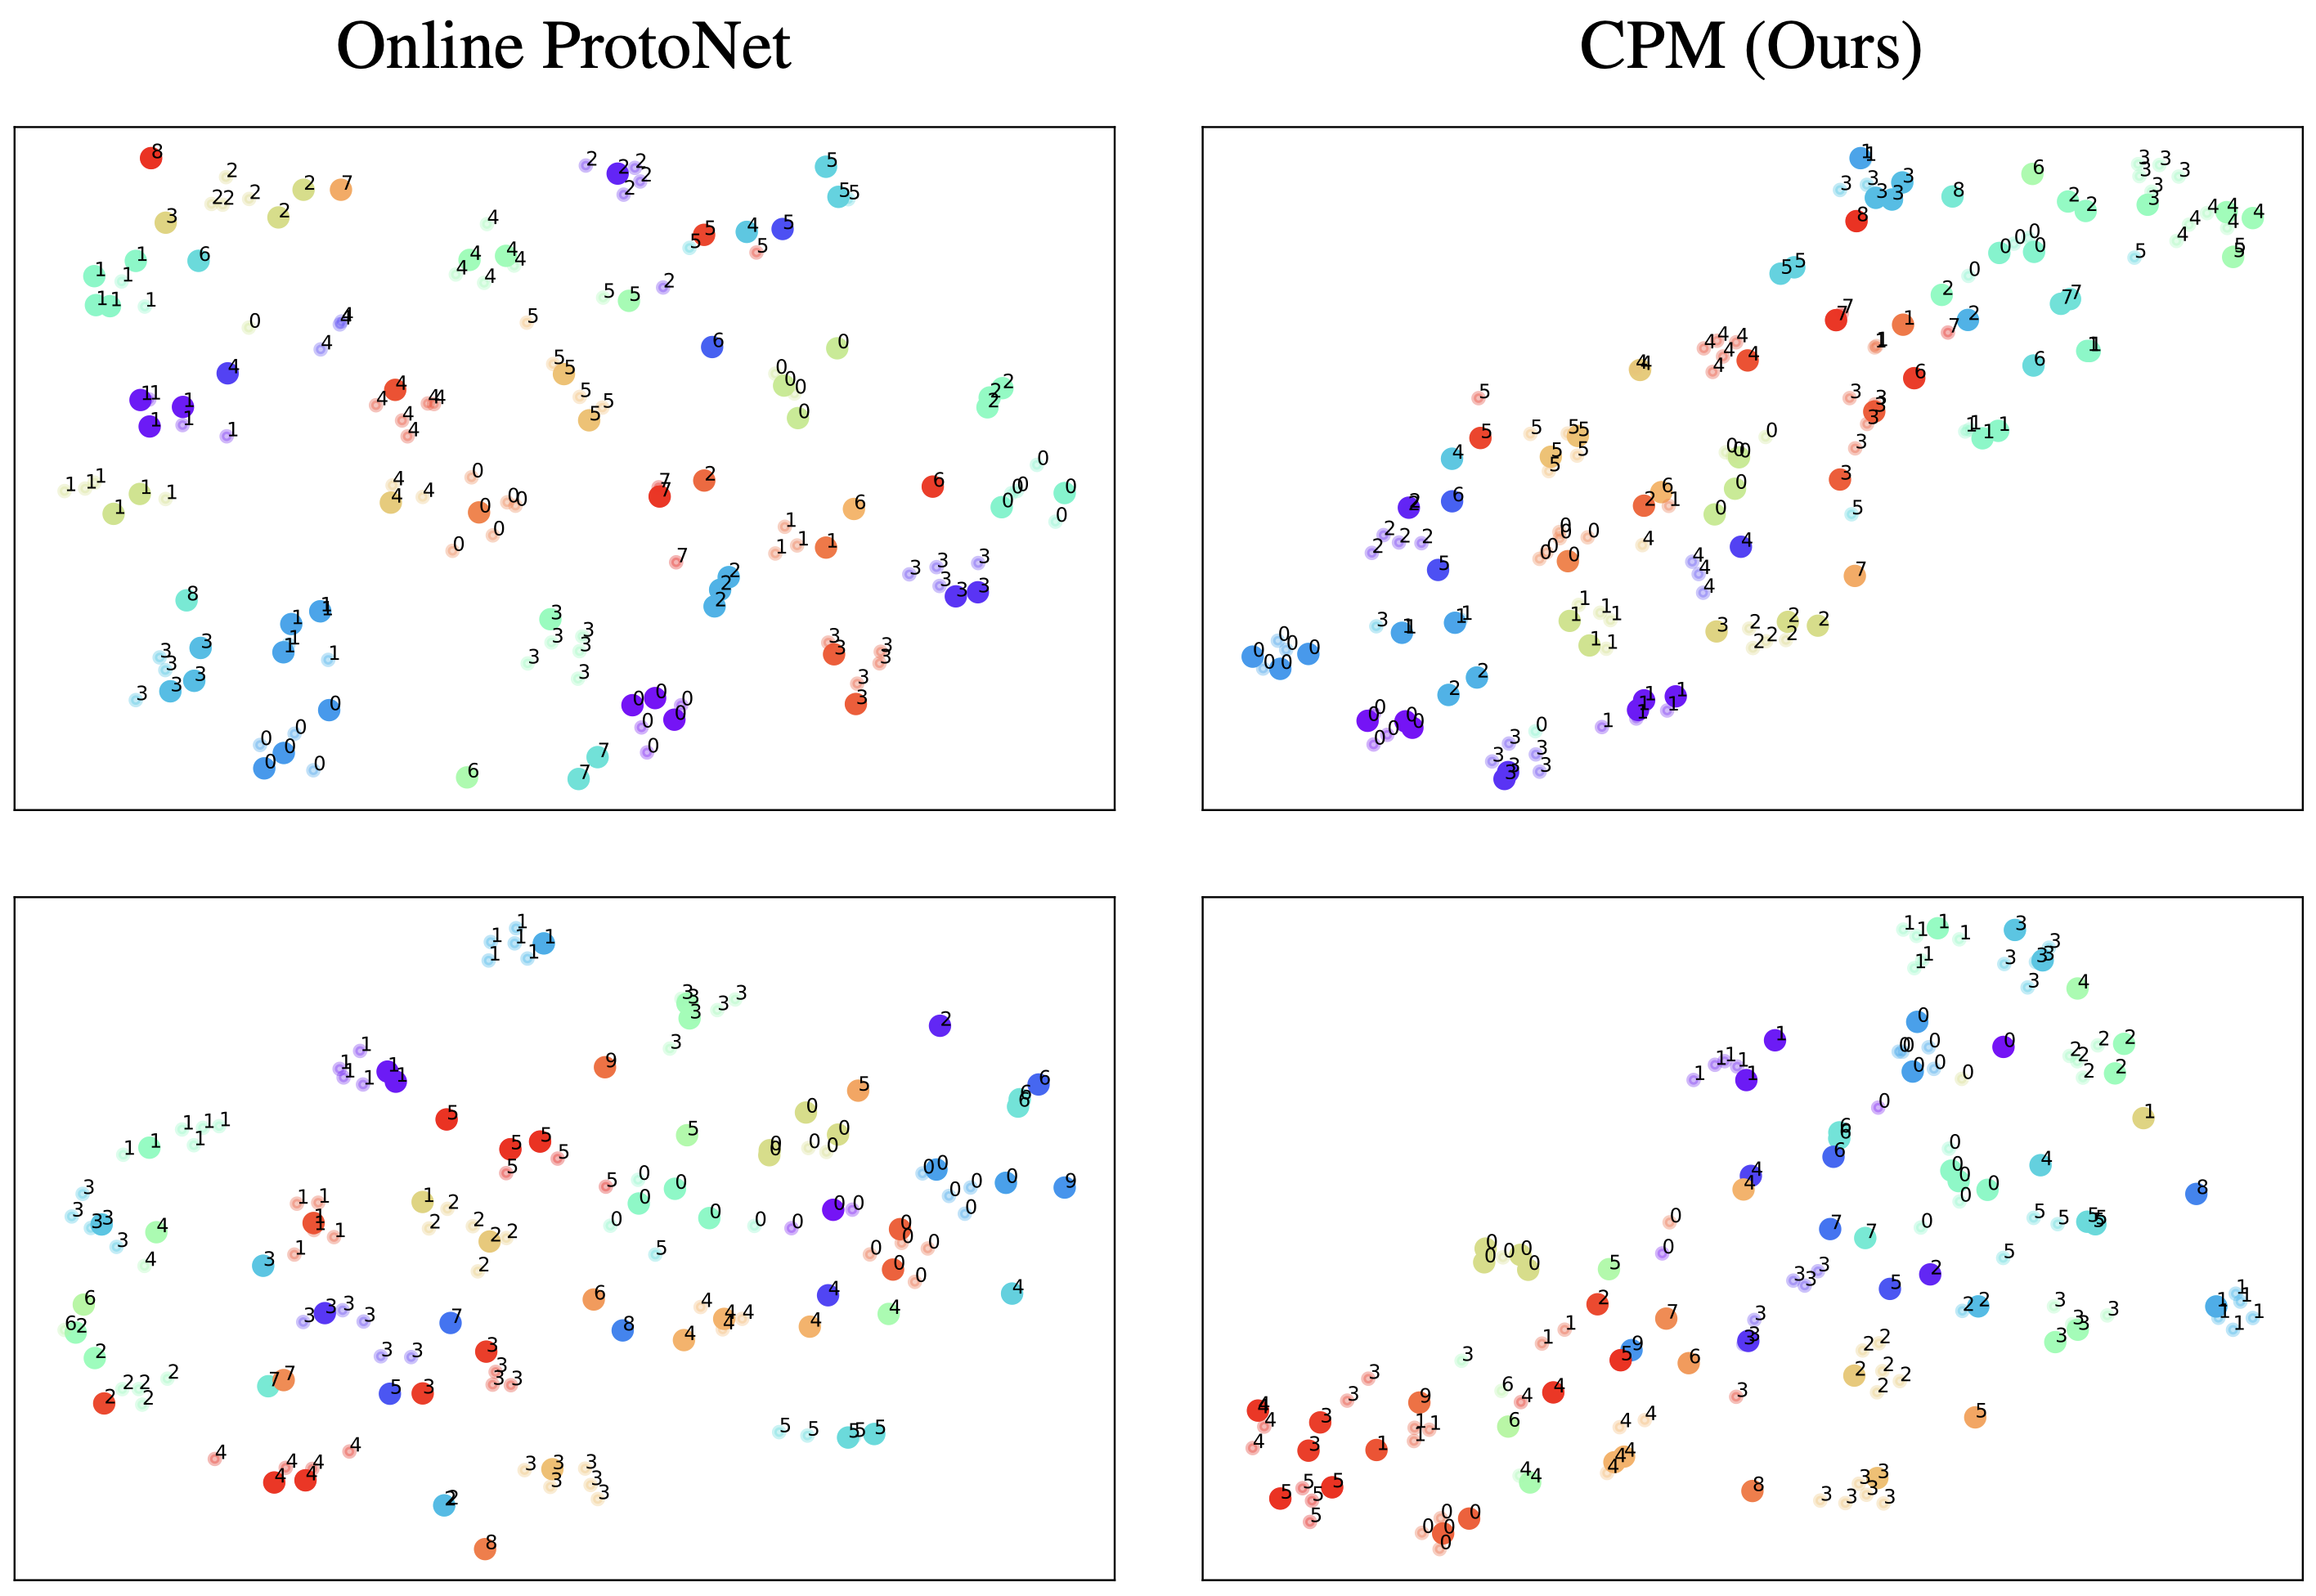
\includegraphics[width=6\linewidth]{figures/omniglot-tsne.png}
\else
    \begin{tabular}{cc}
    Online ProtoNet & CPM (Ours) \\
    \includegraphics[height=3.8cm, trim={2.5cm 1cm 2cm 1cm}, clip]{figures/omniglot-protonet-tsne/tsne-003.pdf}
    &
    \includegraphics[height=3.8cm, trim={2.5cm 1cm 2cm 1cm}, clip]{figures/omniglot-cpm-tsne/tsne-003.pdf}
    \\
    \includegraphics[height=3.8cm, trim={2.5cm 1cm 2cm 1cm}, clip]{figures/omniglot-protonet-tsne/tsne-008.pdf}
    &
    \includegraphics[height=3.8cm, trim={2.5cm 1cm 2cm 1cm}, clip]{figures/omniglot-cpm-tsne/tsne-008.pdf}
    \end{tabular}
\fi
\caption{\textbf{Embedding space visualization of \ourchar{} sequences using t-SNE~\citep{tsne}}. Different color
denotes different environments. Text labels (relative to each environment) are annotated beside the
scatter points. Unlabeled examples shown in smaller circles with lighter colors. \textbf{Left:}
Online ProtoNet; \textbf{Right:} CPM. The embeddings learned CPM model shows a smoother transition
of classes based on their temporal environments.}
\label{fig:tsne}
\end{figure}


\subsection{Control Parameters vs. Time}
Finally we visualize the control parameter values predicted by the RNN in
Figure~\ref{fig:betagamma}. We verify that we indeed need two sets of $\beta$ and $\gamma$ for read
and write operations separately as they learn different values. $\beta^w$ is smaller than $\beta^r$
which means that the network is more conservative when writing to prototypes. $\gamma^w$ grows
larger over time, which means that the network prefers a softer slope when writing to prototypes
since in the later stage the prototype memory has already stored enough content and it can grow
faster, whereas in the earlier stage, the prototype memory is more conservative to avoid embedding
vectors to be assigned to wrong clusters.

% !TEX root = ../supp.tex
\begin{figure}
\centering
% \vspace{-0.1in}
\iflatexml
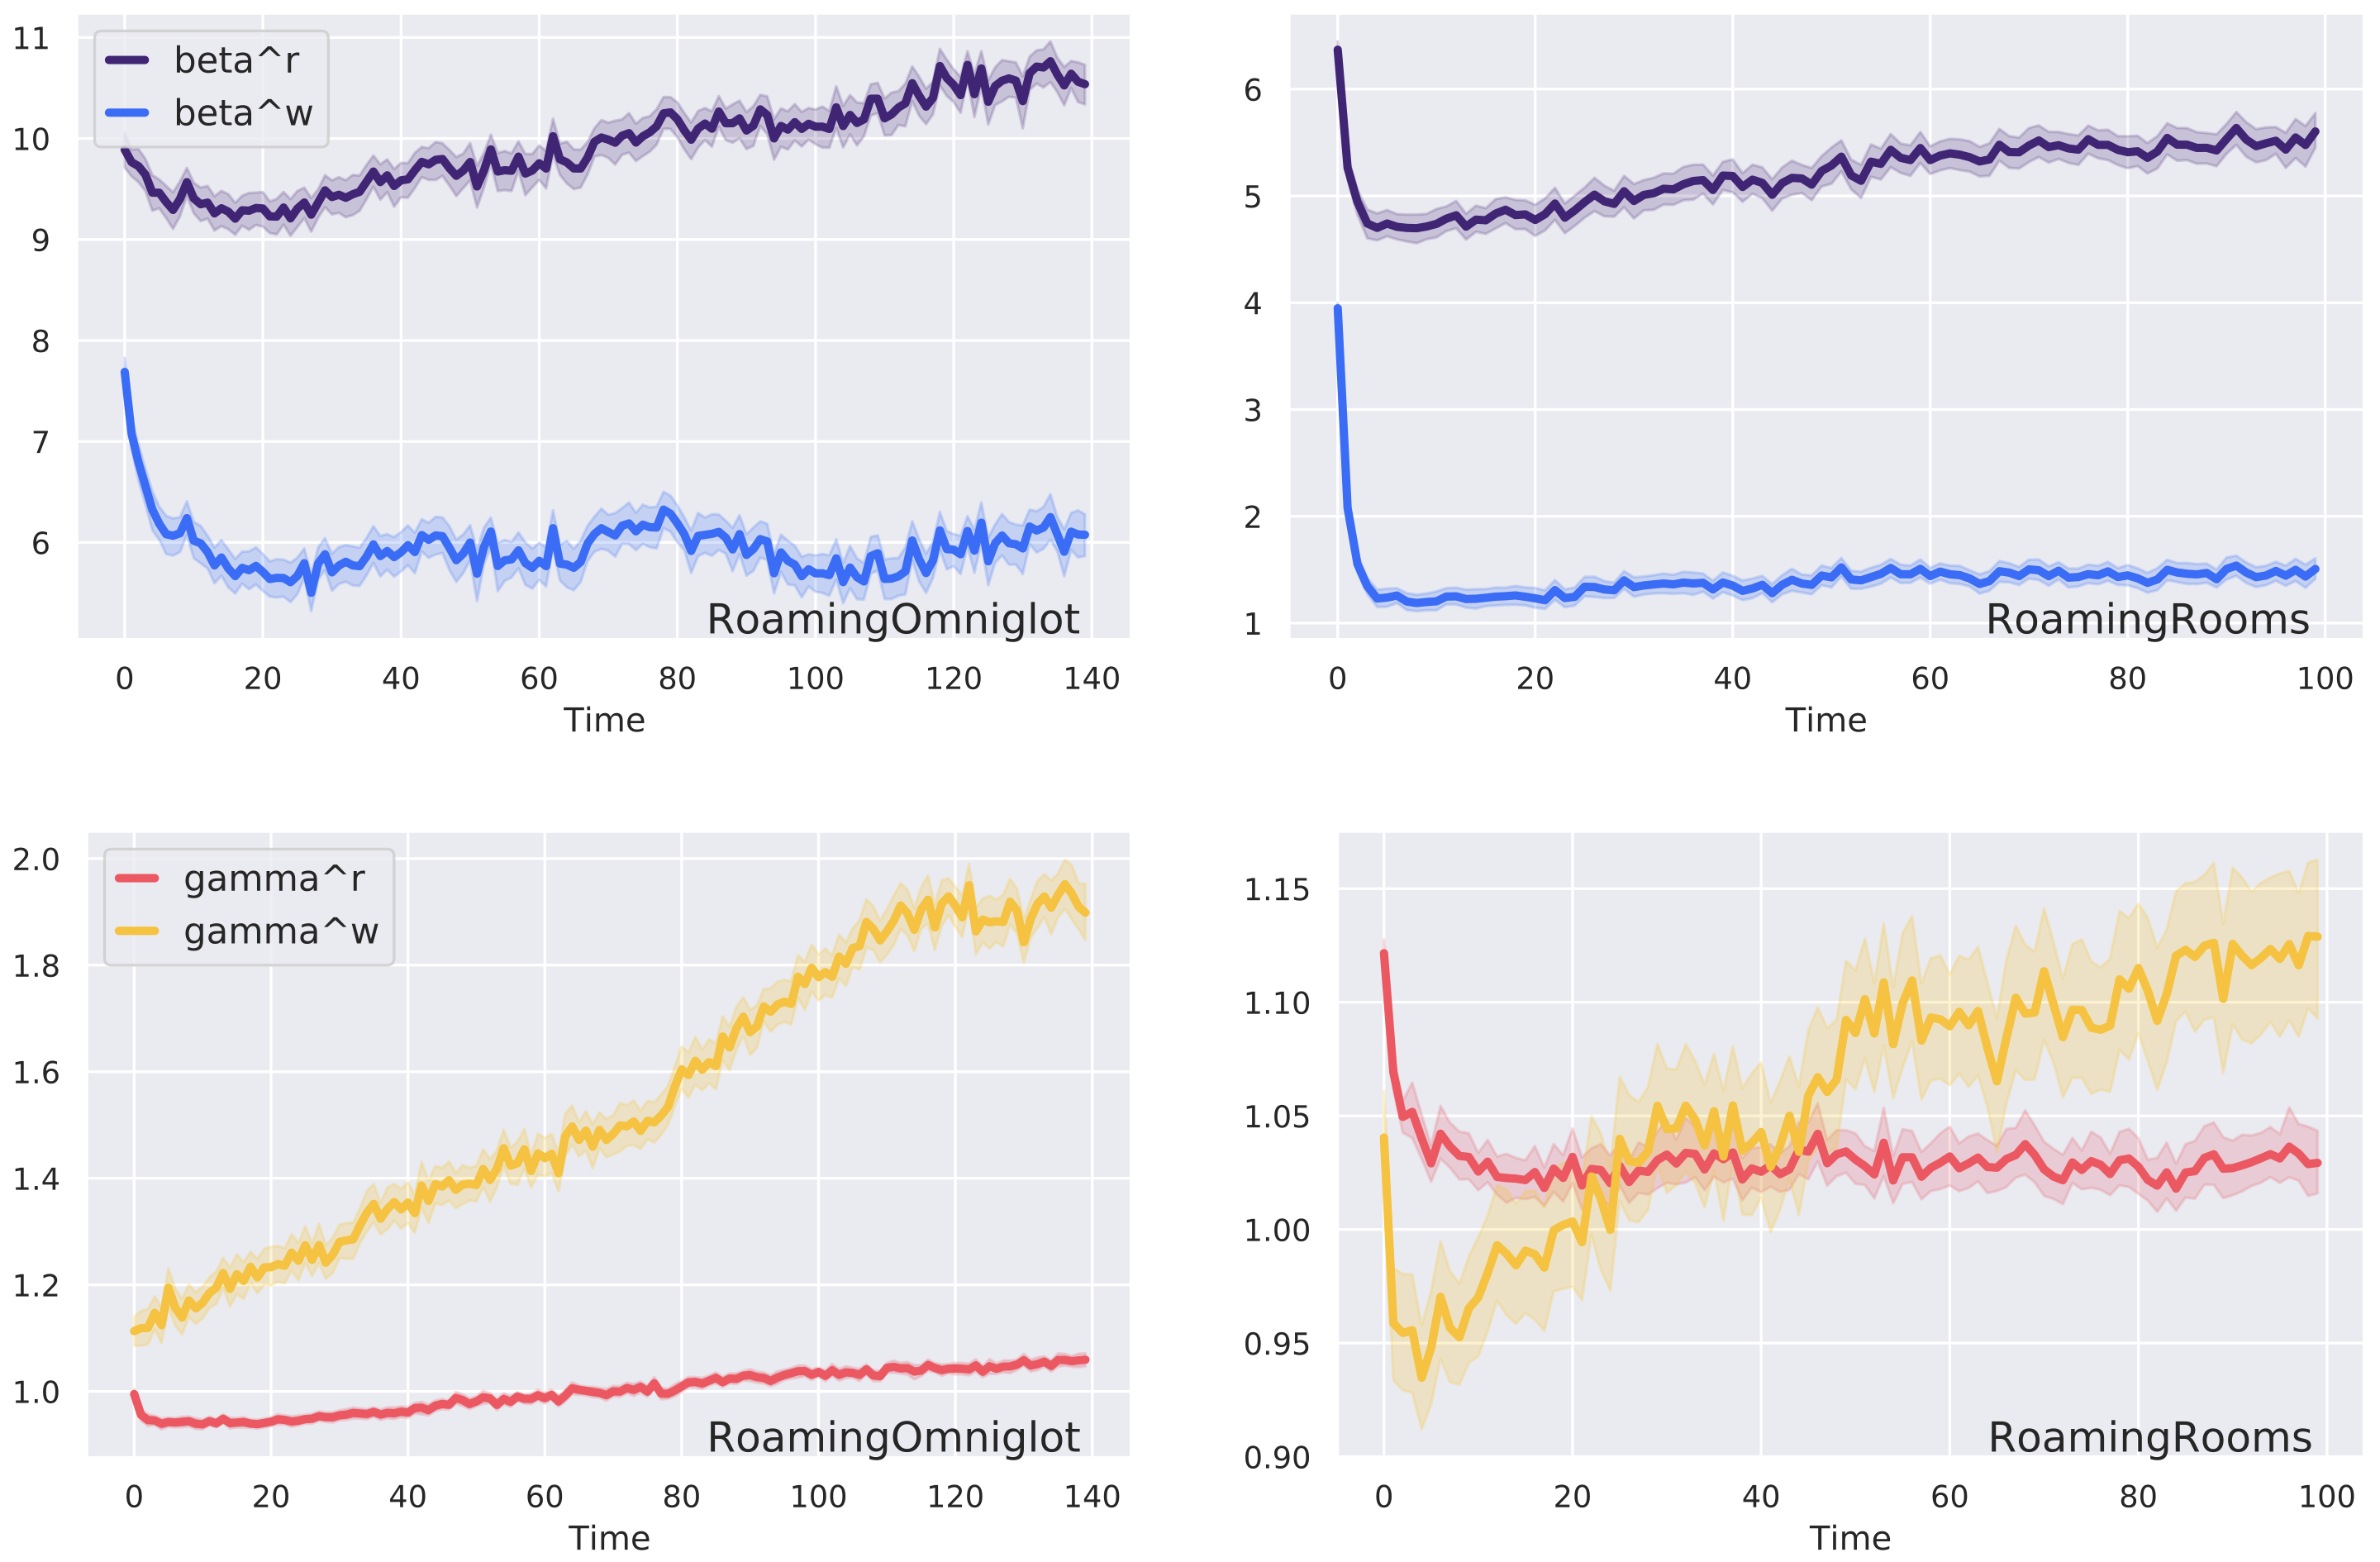
\includegraphics[width=6\linewidth]{figures/beta-gamma.png}
\else
\begin{tabular}{cc}
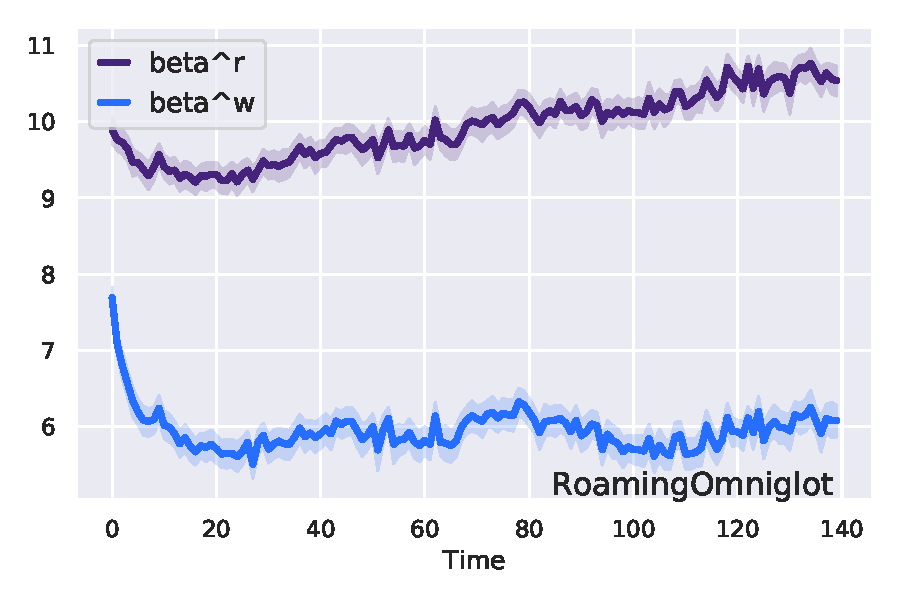
\includegraphics[height=4.0cm,trim={0.3cm 0cm 0.5cm 0},clip]{figures/omniglot-beta.pdf}
\quad
&
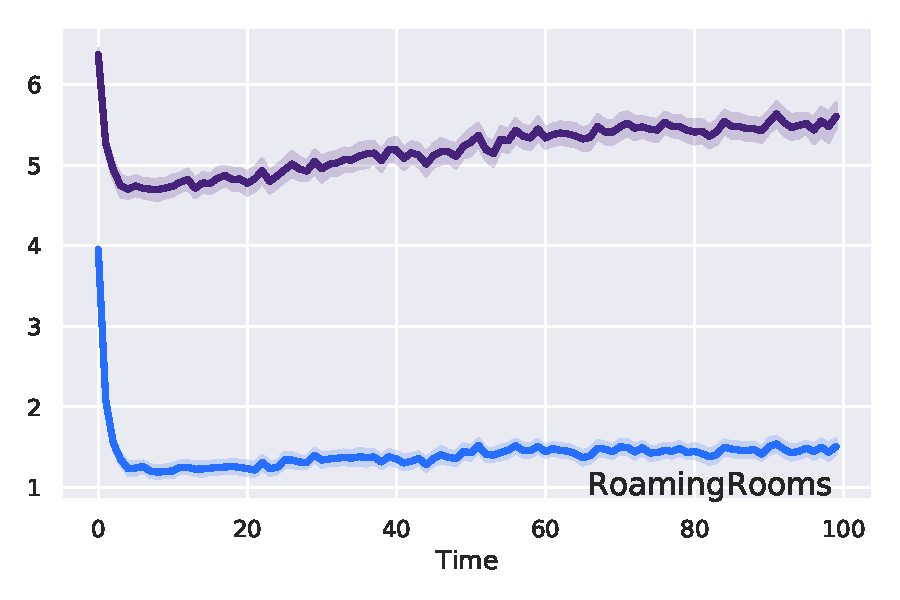
\includegraphics[height=4.0cm,trim={0.3cm 0cm 0cm 0},clip]{figures/matterport-beta.pdf}
\\
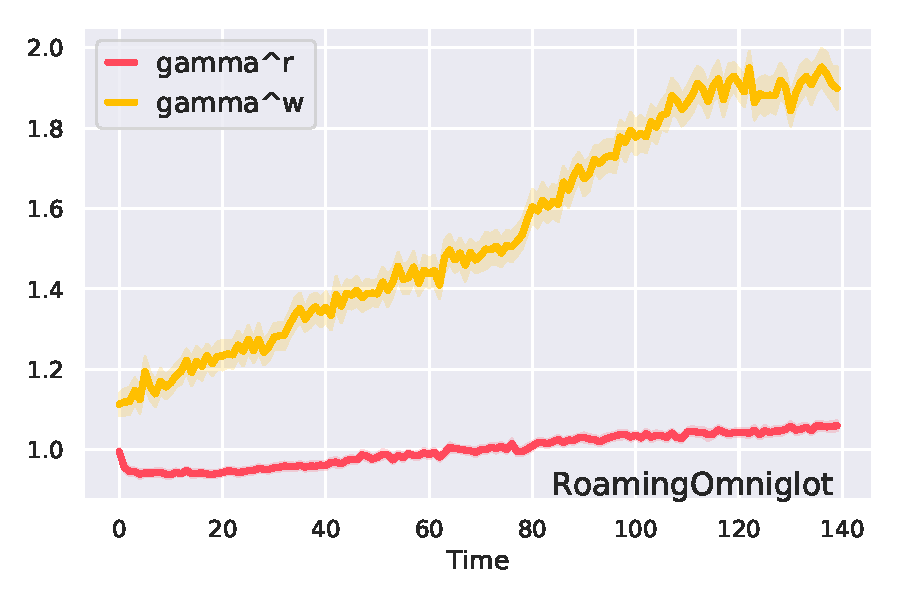
\includegraphics[height=4.0cm,trim={0.3cm 0cm 0.5cm 0},clip]{figures/omniglot-gamma.pdf}
\quad
&
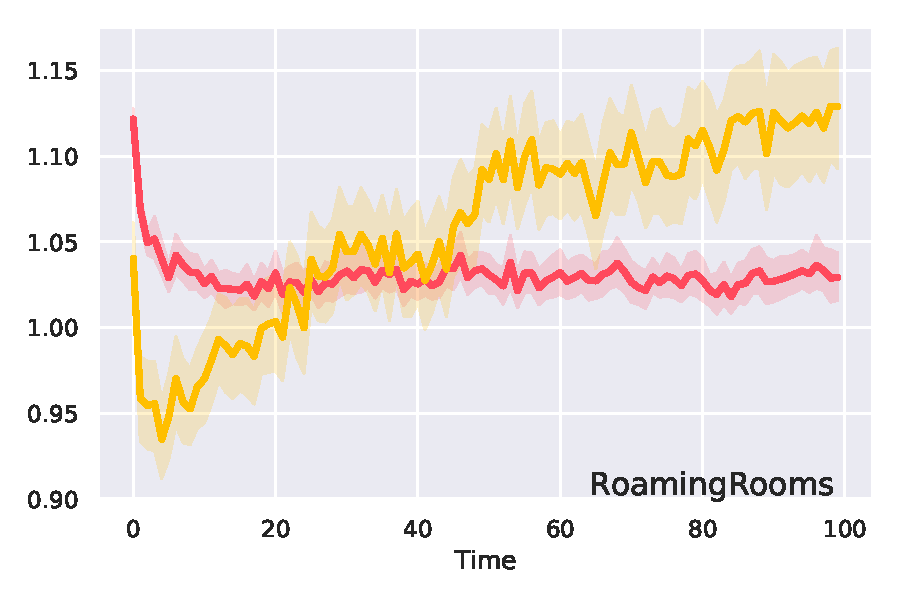
\includegraphics[height=4.0cm,trim={0.3cm 0cm 0cm 0},clip]{figures/matterport-gamma.pdf}
\\
\end{tabular}
\vspace{-0.1in}
\fi
\caption{\textbf{CPM control parameters ($\beta^{r,w}, \gamma^{r,w}$) vs. time.}
\textbf{Left:} \ourchar{} sequences; \textbf{Right:} \ourroom{} sequences; \textbf{Top:}
$\beta^{r,w}$ the threshold parameter; \textbf{Bottom:} $\gamma^{r,w}$ the temperature parameter.}
\label{fig:betagamma}
\end{figure}



%\end{document}
